\documentclass[a4paper, titlepage, openright]{book}

\usepackage[english]{babel}
\usepackage{frontespizio}
\usepackage{amsmath}
\usepackage{amsthm}
\usepackage[linesnumbered,ruled,vlined]{algorithm2e}
\usepackage{textcomp}
\usepackage{mathtools, nccmath}
\usepackage[left=3cm,right=2cm,top=3cm,bottom=2cm]{geometry}
\usepackage{rotating}
\usepackage{subfigure}
\usepackage{url}

% force page number on page bottom part
\usepackage{fancyhdr} 
\fancyhf{}
\cfoot{\thepage}
\pagestyle{fancy}

% These Commands create the label style for tables, figures and equations.
\usepackage[labelfont={footnotesize,bf} , textfont=footnotesize]{caption}
\captionsetup{labelformat=simple, labelsep=period}
\newcommand\num{\addtocounter{equation}{1}\tag{\theequation}}
\renewcommand{\theequation}{\arabic{equation}}
\makeatletter
\renewcommand\tagform@[1]{\maketag@@@ {\ignorespaces {\footnotesize{\textbf{Equation}}} #1.\unskip \@@italiccorr }}
\makeatother
\setlength{\intextsep}{10pt}
\setlength{\abovecaptionskip}{2pt}
\setlength{\belowcaptionskip}{-10pt}

\renewcommand{\textfraction}{0.10}
\renewcommand{\topfraction}{0.85}
\renewcommand{\bottomfraction}{0.85}
\renewcommand{\floatpagefraction}{0.90}

% This styles the bibliography and citations.
\usepackage{natbib}
\setlength\bibindent{2em}
\makeatletter
\setlength{\bibsep}{0pt plus 0.3ex}

% redefine chapter -> no labeling with 1, 2, etc.
\newcommand{\mychapter}[2]{
    \setcounter{chapter}{#1}
    \setcounter{section}{0}
    \chapter*{#2}
    \addcontentsline{toc}{chapter}{#2}
}

% define tools name
\newcommand{\grafimo}{GRAFIMO\xspace}
\newcommand{\crisprme}{CRISPRme\xspace}
\newcommand{\motifraptor}{MotifRaptor\xspace}
\newcommand{\crisprbean}{CRISPR-bean\xspace}

% table of contents will contain also subsections
\setcounter{tocdepth}{2}

% change Bibliography into References
\AtBeginDocument{\renewcommand{\bibname}{References}}

% set input and output for algorithm2e
\SetKwInput{KwInput}{Input}                
\SetKwInput{KwOutput}{Output} 

\begin{document}
% -----  title page
\begin{frontespizio}
	\Universita {Verona}
	\Dipartimento {Informatica}
	\Scuola {Ph.D. in Computer Science}
	\Annoaccademico {2022--2023}
	\Titoletto {Third Year Report}
	\Titolo {Predicting genetic variants imapct on genomic regulatory elements and CRISPR genome editing}
	\Candidato [VR456869]{Manuel Tognon}
	\NCandidato {Student}
	\NRelatore {Supervisor}{}
	\Relatore {Prof. Rosalba Giugno}
	\NCorrelatore {Cosupervisor}{}
	\Correlatore{Prof. Luca Pinello}
\end{frontespizio}
% ------  table of contents, index of figures and tables
\tableofcontents
\listoffigures
\listoftables
% ------ Introduction
\mychapter{1}{Introduction}
Omics sciences have swiftly emerged as fundamental tools for informing medical decisions. They serve as the foundational pillars supporting precision or personalized medicine \citep{ginsburg2009genomic}.  The evolution and enhancements in sequencing technologies have brought about a profound transformation, substantially improving both the quantity and quality of available omics data. This technological progress has had a profound impact, drastically reducing the costs associated with analyses involving omics data. Furthermore it has empowered the accumulation of large dataset, even for individual patients \citep{voelkerding2009next}.  Individual-specific omics data serve as a priceless asset for capturing the distinctive biological attributes,  or biomarkers, that define individuals and even offer insights into potential medical conditions, including diseases. Among these biomarkers, genetic variants hold a pivotal position, operating at the level of DNA sequences. Genetic variants can be located within genes (coding regions), or in other genomic regions (non-coding regions). in the complex landscape of cellular regulation, non-coding genetic variants frequently play important roles in the epigenetic machinery that governs the cellular environment \citep{maurano2012systematic}. While interpreting the functional impact of genetic variants mapped within coding regions on the cellular environment is often straightforward and widely explored in the existing literature, non-coding variants functional interpretation presents challenges.  We refer to the genomic regions governing the cellular environment as genomic regulatory elements (GREs). Currently, several computational tools designed to predict the effects of genetic variants within gene sequences are available to the scientific community.  However,  while these tools are valuable in assessing genetic variants impacts at broader level, they often fall short when it comes to accomodating the requirements of precision genomics.  In the evolving landscape of precision medicine, ther is a growing need for computational resources that can seamlessly  integrate individual-oriented aspects into their analyses.  Moreover, since genomics plays an increasingly central role in healthcare decision-making, the development of more individual centric computational tools becomes fundamental. We addressed these challenges by proposing innovative algorithms and computational tools tailored for the analysis of genetic variant impact on GREs and CRISPR genome editing, at broad and individual-specific levels. Our primary focus has been on creating haplotype- and individual-aware methods, aligning with the growing demand for individual-centric genomics applications.  Our research focused on developing novel algorithms designed to discover and find transcription factor binding sites (TFBSs) within DNA sequences, accounting for individual- and cell type-specific genetic variants.  We propose a novel computational model to represent TFBSs called MotifGraphs, which employs graph data structures to efficiently represent genetic diversity between binding sites from different individuals or cell types, without sacrificing interpretability.  To address the effects of genetic variants on TFBSs, we developed two novel algorithms \grafimo \citep{tognon2021grafimo} and \motifraptor \citep{yao2021motif}. \grafimo searches for occurrences of known TFBSs genome graphs \citep{paten2017genome}, while accounting for for individual haplotypes and genetic variants. \motifraptor predicts and annotates genetic variants impact on TFBSs integrating different omics data, such as chromatin accessibility, gene expression and GWAS summary statistics. Additionaly we introduced \crisprme \citep{cancellieri2023human}, a tool designed to CRISPR off-targets and avaluate the potential impact of individual genetic variants on target specificity.  Importantly,  \crisprme considers single-nucleotide variants, accomadate bona fide haplotypes and handles spacer:protospacer mismatches and bulges. This tool is specifically designed to perform individuals-oriented analyses, considering the wide genetic diversity present in different populations.

% ------ Transcription Factors
\mychapter{2}{Transcription Factors}
Transcription factors (TFs) (\textbf{Fig.\ref{fig:ctcf_dna}}) are fundamental regulatory proteins playing a key role in regulating the transcriptional state,  cellular differentiation and developmental state of cells  \citep{lambert2018human, reimold2001plasma, whyte2013master}.  In human, approximately 1600 proteins are recognized as TFs \citep{babu2004structure}.  This number accounts for roughly 8\% of all human genes, highlighting the critical role played by TFs orchestrating genetic regulation. TFs exhibit their regulatory prowess by often collaborating in a coordinated manner to influence gene expression. This collaborative orchestration is vital for fine-tuning and precisely controlling cellular process.  Moreover, TFs display a remarkable versatility as they govern the activity of multiple genes across different cell types \citep{lambert2018human}.  TFs exhibit a modular structure, that is divided into three distinct domains \citep{latchman1997transcription}.  (i) The DNA binding domain directs the TF to its precise target site on the genome.  Through a specific recognition of DNA sequences, the DNA binding domain enables the TF to dock onto regulatory regions located across the genome. (ii) the activation domain facilitates interactions between the TF and other transcriptional regulators. By engaging with different co-factors and regulatory proteins, the activation domain plays a crucial role modulating gene expression, often acting as a bridge between the factor and the transcriptional machinery.  (iii) The signal sensing domain captures external signals and transmits them to the broader transcriptional complex. These signals can originate from different sources, including cellular cues and environmental stimuli, and are essential for fine-tuning the TF regulatory actions in response to changing conditions.  The interplay between these three domains allows TFs to function as highly versatile and adaptable components of the gene regulation machinery, responding to both internal and external cues to precisely control gene expression in a dynamic and context-dependent manner. TFs exert their function through different strategies. (i) TFs can either facilitate the recruitment of RNA polymerase to gene promoter regions, thus promoting transcription initiation, or block RNA polymerase access \citep{fuda2009defining}. (ii) TFs play a crucial role in shaping chromatin landscape by weakening DNA-histone interactions,  increasing DNA accessibility and consequently facilitating gene expression. (iii) Some TFs catalyze histone deacetylation \citep{liu2016beyond}, by removing acetyl groups from histones, thus promoting a more compact chromatin structure and consequently reducing gene transcription. (iv) Other TFs enhance DNA-histone interactions, leading to a more tightly packed chromatin structure and consequently repressing gene expression. Therefore,  by binding short DNA sequences ($\sim$6-20 nucleotides  \citep{stewart2012transcription}), known as transcription factor binding sites (TFBSs), they finely regulate gene expression in a cell-specific manner.  TFBSs are located within gene promoters \citep{whitfield2012functional} or in more distant regulatory elements such as enhancers, silencers, or insulators \citep{gotea2010homotypic,lemon2000orchestrated,nolis2009transcription}.  While TFBS often exhibit recurring sequence patterns, referred to as \emph{motifs}, TFs display a remarkable ability to bind to similar but not identical sequences, often differing by just a few nucleotides. The precise configuration of TFBS, coupled with the local chromatin structure, plays a pivotal role in fine-tuning TFs' regulatory functions within cells \citep{mendenhall2013locus,maurano2015large}. During the process of DNA binding, Transcription Factors harness a combination of electrostatic and Van der Waals forces. Although TFs exhibit high specificity in binding to their target sequences, not every nucleotide within the binding site directly interacts with the TF. These interactions vary in strength, resulting in TFs binding not to a single specific sequence but to a closely related subset of targets. However, the sequence composition of the TFBS decisively dictates the strength of the TF-DNA interaction, known as binding affinity. Numerous studies have established links between different diseases and cancer types and genetic variants occurring within TFBS \citep{docquier2005heightened, katainen2015ctcf, yu2019gata1}. Furthermore, variants within TFBS can disrupt the precise regulation of gene expression by TFs, potentially affecting the entire cellular environment and even propagating effects to neighboring cells. Moreover, the misregulation of gene expression governed by TFs caused by variants occurring in TFBS could affect the entire cell environment and be propagated to neighboring cells. Therefore, identifying such regulatory motifs would provide fundamental insights on the complex mechanisms governing gene expression and the cell environment.
\begin{figure}
	\centering
	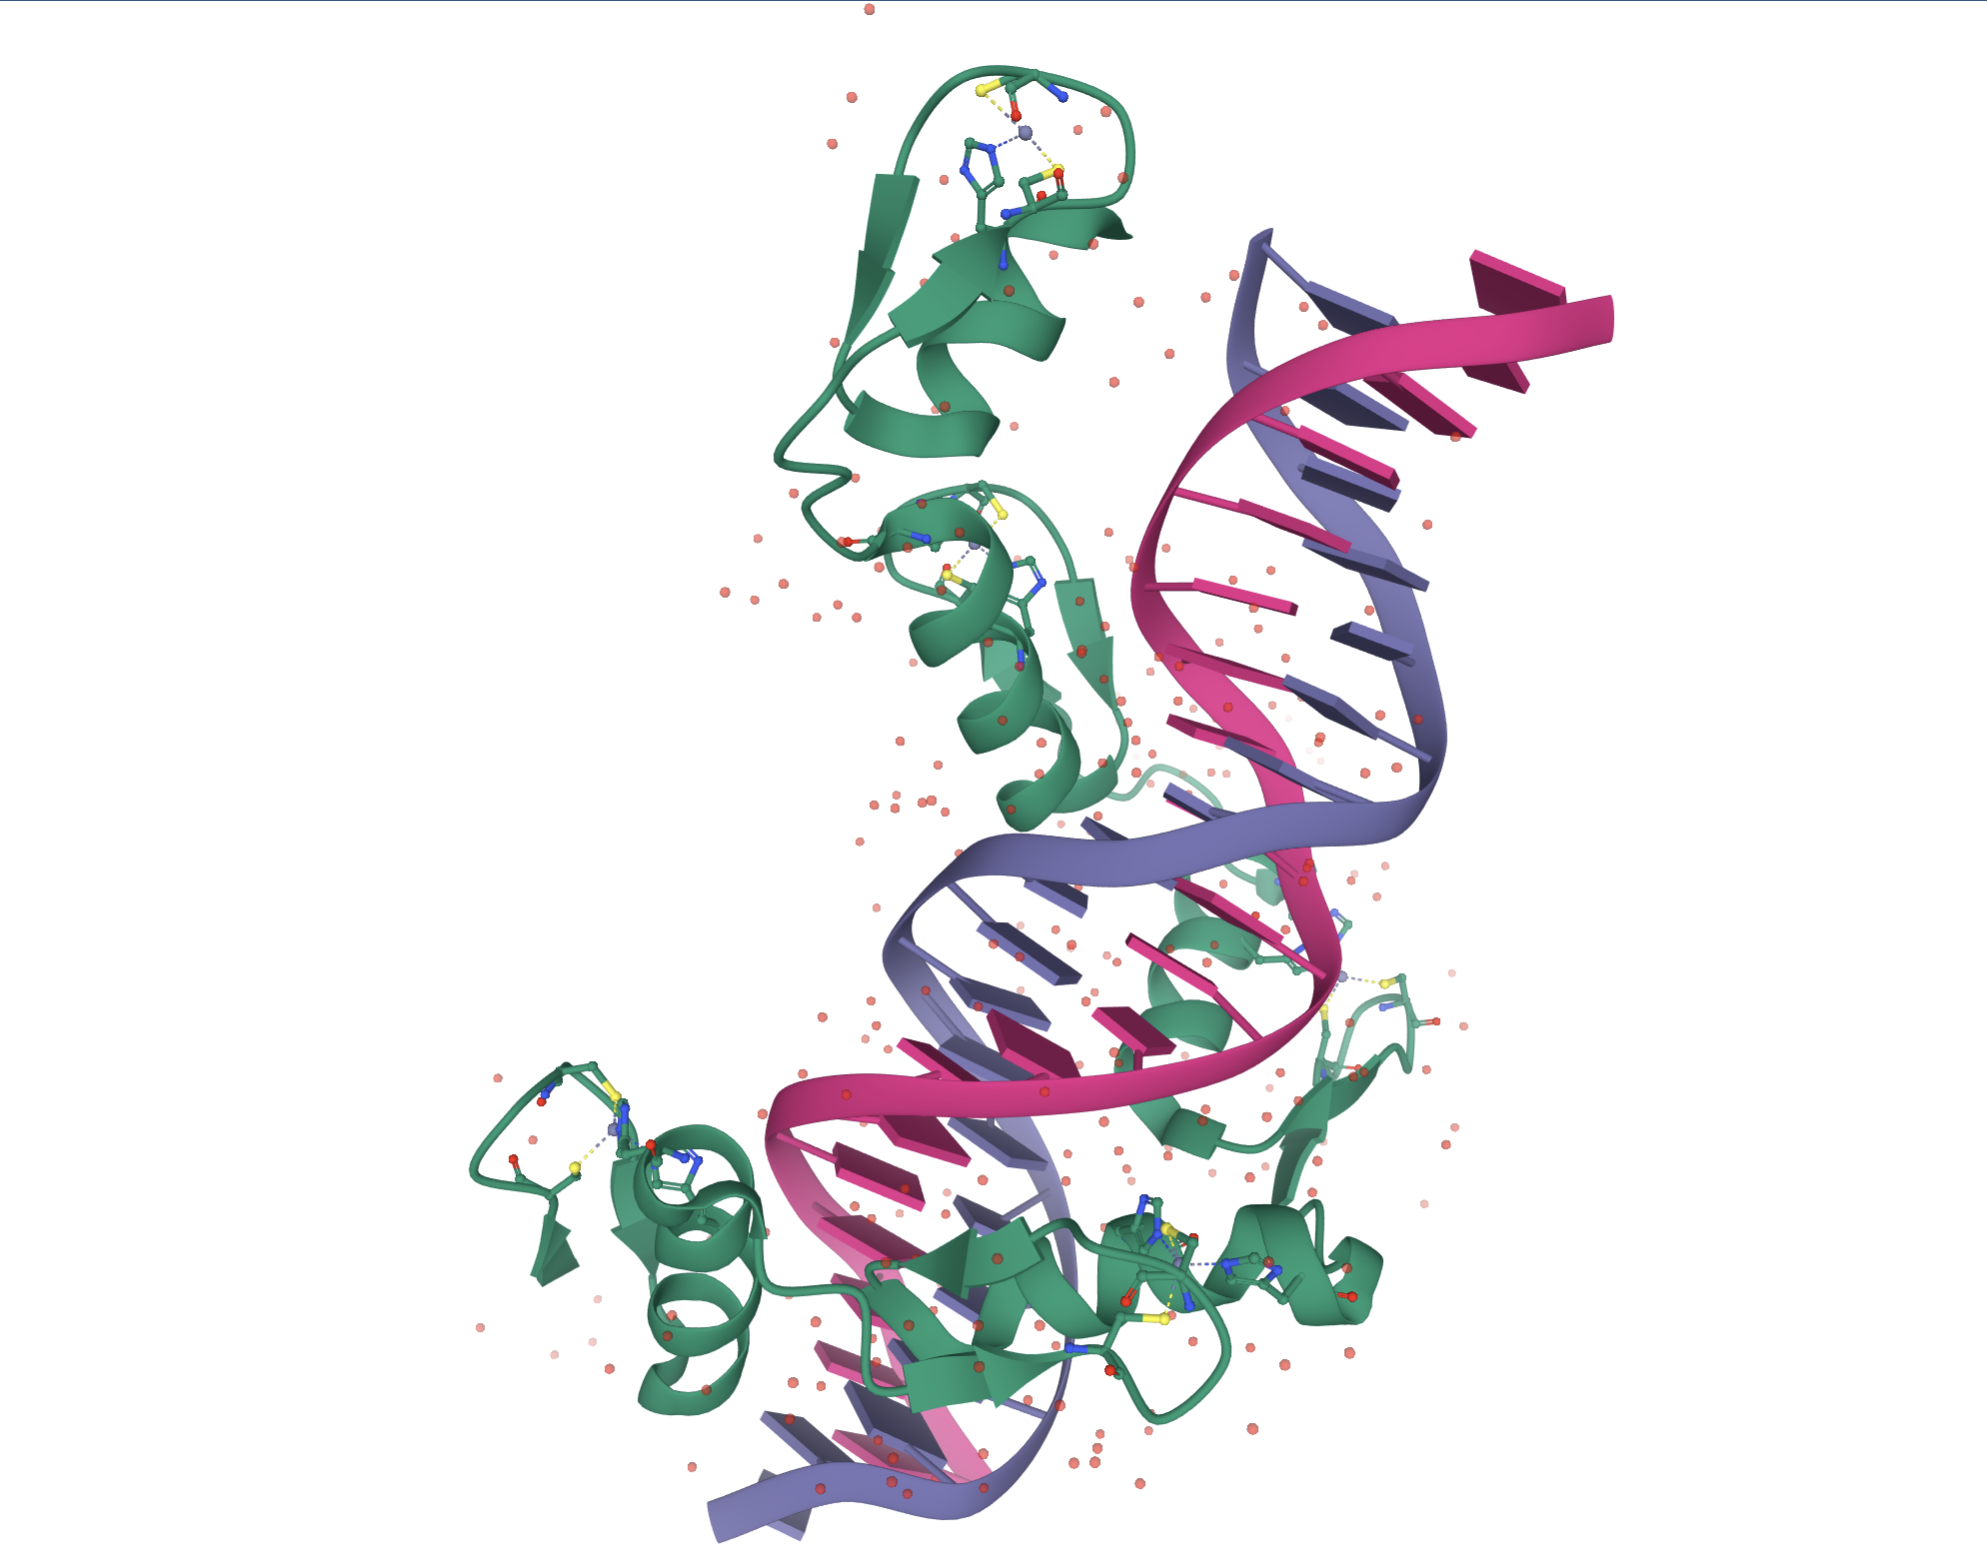
\includegraphics[width=\textwidth]{figures/ctcf_dna.png}
	\caption[A human transcription factor (CTCF) binding its DNA target sequence.]{\textbf{A human transcription factor (CTCF) binding its DNA target sequence.}}
	\label{fig:ctcf_dna}
\end{figure}
% ---- Discovering Transcription Factor Binding Site motifs
\section{Discovering Transcription Factor Binding Site motifs}
Several experimental assays have been developed to determine the binding site sequences of TFs in living cells or organisms (\emph{in vivo}), or in test-tubes using synthetic or purified components (\emph{in vitro}) \citep{jolma2011methods}. Early methods, like electrophoretic mobility shift assay (EMSA) \citep{garner1981gel} or footprinting \citep{hampshire2007footprinting},  generally analyze a relatively small number of target sequences to find TFBS. As a result, they return small datasets of bound sequences. \emph{In vitro} and \emph{in vivo} high-throughput protocols such as PBM, SELEX or ChIP methods \citep{berger2006compact,jolma2010multiplexed,collas2008chop}, facilitated the analysis of most target sites for factors of interest. As a result, large datasets of bound sequences have been generated, presenting an unprecedented opportunity to study and determine the TF binding landscapes. Experimental assays can recover the sequences bound by TFs along with their relative or absolute binding affinity. However, such datasets can incorrectly report unbound sequences as binding sites. In addition, the assays usually capture extra nucleotides in target sites, reducing data resolution and making manual analysis challenging. Motif discovery algorithms provide a computational framework to analyze these large datasets generated by experimental assays, discovering the sequences potentially bound by TFs and predicting their affinities \citep{pavesi2004silico,tompa2005assessing,d2006does,das2007survey,zambelli2013motif,tognon2023survey}. Given a sequence dataset, these algorithms typically recover sets of short and similar sequence elements. The prioritized sequence elements are later used to construct a motif model, summarizing the diverse binding site configurations observed among the prioritized sequences, and encoding their recurrent patterns and similarities (\textbf{Fig.\ref{fig:md} (A)}). Several methods and models have been proposed to discover and represent TFBS motifs. Position weight matrices (PWMs) \citep{stormo2000dna} are the most popular models. PWMs are simple yet powerful and interpretable models, encoding the probability of observing a given nucleotide in each TFBS position. However, PWMs have some limitations, like the assumption of independence among the binding site positions. Therefore, several alternative motif models have been proposed \citep{siddharthan2010dinucleotide,gorkin2012integration,he2021survey} , as described below. The derived motif models can be employed in many downstream analyses, like searching potential binding site occurrences in regulatory genomic sequences, predicting the sets of genes regulated by the investigated TFs or assessing how genetic variants could affect their binding landscape.
% -- Experimental methods to discover Transcription Factor Binding Sites
\begin{table}
	\centering
	\begin{tabular}{|p{2.4cm}|p{4cm}|p{1.75cm}|p{1.5cm}|p{1cm}|p{2.3cm}|p{2cm}|}
		\hline
		\textbf{Experimental assay}& \textbf{Description}&\textbf{Output}&\textbf{\emph{De novo} motif discovery capability}& \textbf{Type}& \textbf{Identification of genomic binding locations}& \textbf{Throughput} \\
		\hline
		Competition EMSA& Bound DNA sequences are identified by observing changes in the electrophoretic migration of DNA sequences through non-denatured polyacrylamide gel& Bound DNA sequences& No. Used to validate known binding sites& \emph{in vitro}& No& Low\\  
		\hline
		DNase footprinting& Pools of DNA sequences are incubated with the TF of interest; then, the DNA is degraded using DNase I. The unbound fragments are cut in all positions, while the bound DNA is protected by the TF& Bound DNA sequences.& No. Used to validate known binding sites.& \emph{in vitro}& No& Low\\
		\hline
		Protein Binding Microarrays& Arrays of $\sim$40 000 spots with short, immobilized DNA sequences are incubated with a tagged TF, and then washed to remove weakly bound proteins. The bound sequences are identified through fluorescence-based detection & Continuous values describing fluorescence intensity on each array spot & Yes. Limited to short motifs ($\sim$12bp)& \emph{in vitro}& No& High\\
		\hline
		HT-SELEX& The TF is added to a pool of randomized DNA fragments. The bound sequences are selected and constitute the starting pool for the next experimental round. The procedure is repeated for several rounds. Sequencing is employed to recover the sequence of the bound DNA fragments & DNA sequences& Yes& \emph{in vitro}& No& High\\
		\hline
		ChIP-based technologies& TF–DNA complexes are cross-linked with formaldehyde and immunoprecipitated employing TF-specific antibodies. The bound sequences are then prioritized employing qPCR microarrays (ChIP-on-Chip) or through sequencing (ChIP-seq). ChIP-exo integrates exonuclease treatment to enhance sequence resolution & Genomic binding location coordinates& Yes. Limited by the inability to distinguish direct and indirect binding& \emph{in vivo}& Yes& Low\\
		\hline
	\end{tabular}
	\caption[\emph{In vivo} and \emph{in vitro} experimental assays to identify and validate transcription factor binding sites.]{\emph{In vivo} and \emph{in vitro} experimental assays to identify and validate transcription factor binding sites}
	\label{table:assays}
\end{table}
\begin{figure}
	\centering
	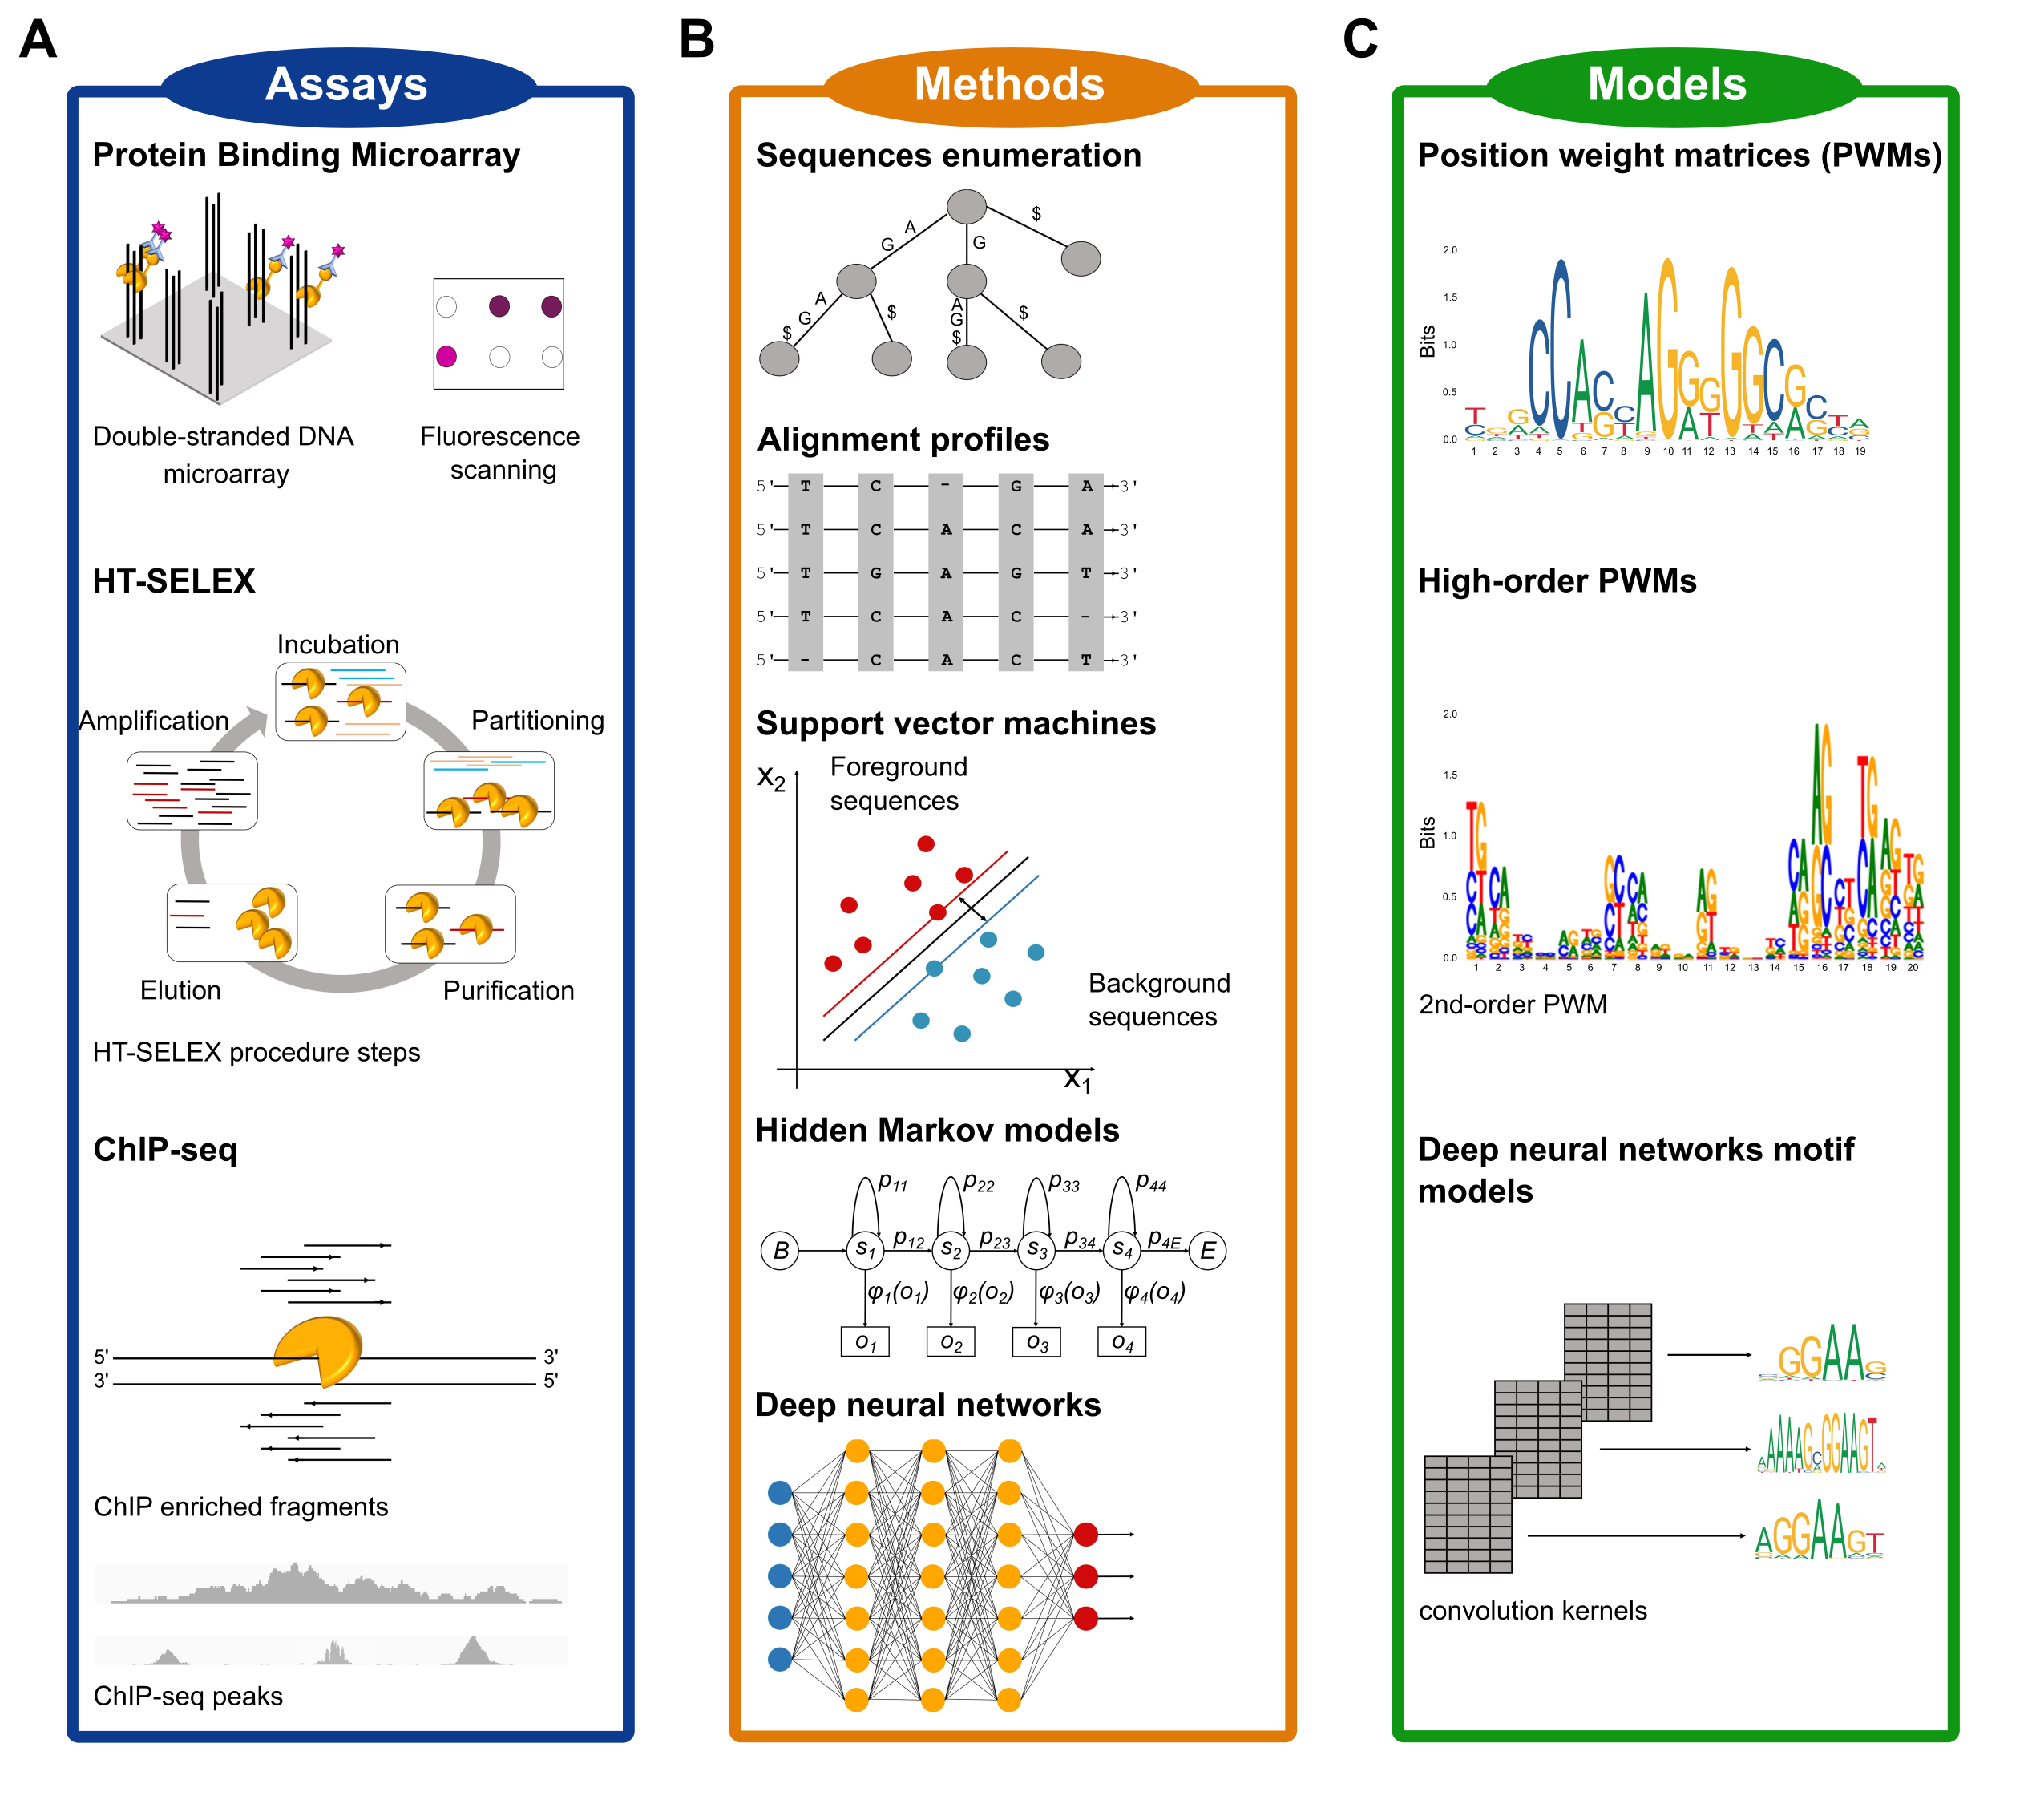
\includegraphics[width=\textwidth]{figures/md.png}
	\caption[Experimental and computational methods to discover TFBS and popular models to represent binding site motifs.]{\textbf{Experimental and computational methods to discover TFBS and popular models to represent binding site motifs.} Protein binding microarray (PBM), HT-SELEX and ChIP-seq have become the most popular assays to determine TF binding preferences and identify their target sites (TFBS) in recent years. Computational motif discovery methods can be grouped into five classes, based on the algorithms employed to discover TFBS: enumerative, alignment-based, probabilistic graphical model-based, SVM-based and DNN-based methods. TFBS sequences prioritized by motif discovery algorithms are encoded in computational models representing the binding preferences of the investigated TFs.}
	\label{fig:md}
\end{figure}
\subsection{Experimental methods to discover Transcription Factor Binding Sites}
During the last decades, several techniques have been introduced to experimentally identify and assess TF binding sites and binding preferences \citep{jolma2011methods} (\textbf{Fig.\ref{fig:md}} and \textbf{Table \ref{table:assays}}). Early studies on TF binding focused their analysis on gene promoters \citep{stormo2000dna} and employed in vitro methods, such as Electro-Mobility Shift Assay (EMSA) \citep{garner1981gel} or DNase footprinting \citep{galas1978dnaase}. EMSA exploits non-denatured polyacrylamide gel properties to separate bound and unbound DNA sequences. DNase footprinting combines EMSA with DNase I cleavage, identifying uncut regions (footprints) due to the protection of the bound TF. Generally, these assays produce datasets of a few hundred of bound sequences, exploring a limited spectrum of TFs binding landscape. Moreover, EMSA and DNase footprinting may be subject to technical constraints that could lead to inaccuracies in the reported sequences and binding preferences \citep{jolma2011methods}.  The introduction of NGS technologies revolutionized the study of TFBS identification by encouraging researchers to develop methods that exploit the power of massively parallel sequencing (\textbf{Fig.\ref{fig:md}}). These methods have two major advantages: (i) they do not require any prior knowledge on the binding site sequence \citep{jolma2011methods, zia2012towards} and (ii) produce datasets of thousands of bound sequences allowing a better characterization of TF binding preferences \citep{stormo2010determining}. Protein binding microarrays (PBMs) \citep{berger2006compact,berger2009universal} recover short TFBS sequences ($\sim$10 bp) and measure TF binding preferences in vitro. In PBMs, a tagged TF is released on a glass slide containing thousands of spots filled with short, immobilized DNA sequences. The tagged TFs are then incubated with fluorescent antibodies against the tag and subsequently washed to remove weakly bound factors. The fluorescence and DNA sequence enrichment are then used to quantify the TF–DNA binding strength and capture the bound sequences. Generally, the recovered sequences do not contain nucleotides flanking the investigated binding sites, producing high-resolution datasets. However, since the number of possible sequences grows as a function of the target length, PBMs can assess only a limited number of target sequences \citep{jolma2011methods, zia2012towards}. PBM analysis is usually constrained to binding sites $\sim$10–12 bp long. HT-SELEX \citep{jolma2011methods,jolma2010multiplexed} is a widely used \emph{in vitro} method, coupling SELEX with high-throughput sequencing. A TF is released on a pool of randomized DNA sequences to allow the factor to select its target sites. The resulting TF–DNA complexes are separated from unbound sequences using affinity capture, and subsequently amplified through polymerase chain reaction (PCR) and sequenced. The resulting DNA library is enriched in binding sites for the studied TF and is used as the starting pool for another SELEX run \citep{jolma2011methods,jolma2010multiplexed}. SELEX does not require any prior knowledge on the target sites of the investigated factor \citep{jolma2013dna}. Since SELEX reaction is typically performed in liquid phase and consequently does not suffer from physical constraints, the sequence space covered by HT-SELEX is often larger than that of PBMs. Moreover, by coupling sequencing with DNA barcode indexing, HT-SELEX allows to analyze hundreds of TFs in parallel. HT-SELEX produces datasets of thousands of high-resolution bound sequences, which include only a few nucleotides flanking the binding sites. However, since the starting DNA library is constituted by randomized sequences, HT-SELEX cannot recover the genomic binding locations for the investigated factor. The introduction of chromatin immunoprecipitation (ChIP) technologies \citep{collas2008chop}. radically changed the study of TFBS binding, enabling the genome-wide identification of regions bound by TFs in vivo. In ChIP, the TF–DNA complexes are cross-linked using formaldehyde. The DNA is then fragmented in $\sim$100–1000 bp long fragments and subsequently immunoprecipitated with antibodies specific for the investigated TF. To recover the bound sequences, the cross-links are reverted. Then, the resulting fragments are amplified through microarray hybridization (ChIP-on-Chip \citep{collas2008chop,pillai2015chip}) or sequencing (ChIP-seq \citep{johnson2007genome,mardis2007chip}). To locate the binding regions, the recovered DNA fragments are mapped onto the genome. After ChIP-seq reads mapping, peak calling algorithms \citep{thomas2017features,guo2012high,zhang2008model} are employed to predict the genomic binding locations for the investigated factor. Peak calling algorithms identify the genomic regions showing greater enrichment in mapped DNA probes with respect to a control experiment and mark those regions as binding locations, or peaks  \citep{pepke2009computation}. ChIP methods produce large datasets of thousands of genomic regions, whose length ranges from few hundreds to thousands of nucleotides, from which we can identify the likely TFBS for the investigated factor. Although ChIP technologies, and particularly ChIP-seq, are currently considered the current ‘golden standard’, they have some limitations. (i) ChIP can detect indirect binding, identifying other TFBS not belonging to the investigated factor \citep{worsley2014non}. (ii) ChIP-seq peaks may be false positives, recovered because of poor antibody quality \citep{pickrell2011false}. (iii) ChIP-seq returns low-resolution datasets, whose sequences include several nucleotides flanking the target TFBS. ChIP-exo  \citep{rhee2011comprehensive} addresses the latter issue, employing a lambda exonuclease to trim ChIP sequences, removing some of the nucleotides flanking the target sites. Alternatively, since most TFs bind their target sequences in open chromatin regions, experimental assays targeting open chromatin like ATAC-seq or DNase-seq \citep{buenrostro2013transposition,john2011chromatin} can be employed to recover in vivo genomic locations likely to contain TFBS. ATAC-seq and DNase-seq are generally employed when the factors binding the target regions are not known.In summary, the current high-throughput in vivo and in vitro assays generate datasets of thousands of sequences potentially containing several possible binding configurations of TFBS, thereby enabling better characterizations of TFs binding landscapes.
% -- Computational methods to discover Transcription Factor Binding Sites
\subsection{Computational methods and models to discover and represent Transcription Factor Binding Sites}
The TFBS motif discovery problem can be formalized as follows. Given a set of positive DNA sequences $S$, obtained from an experimental assay targeting a certain TF, and a set of negative sequences $B$ the goal is to find one or more recurrent, short and similar subsequences in $S$ that maximize the discriminatory power between $S$ and $B$. Such subsequences are called patterns or motifs and are likely bound by the investigated TF.  The negative set $B$ can contain randomly generated or selected genomic sequences, with similar nucleotide content and length of those in $S$. The retrieved patterns are used to construct and train a computational model $M$ (motif model), representing the discovered motif. These models can then be used to identify new potential binding sites, given a new set of sequences, and to predict the strength of the TF–DNA binding. Motif discovery can be considered a classification or a regression problem, depending on the type of data used to train $M$ \citep{tognon2023survey}.  The datasets derived by experimental assays like ChIP-seq or HT-SELEX provide hundreds or thousands of sequences containing binding sites. In this setting, motif discovery becomes a classification problem. In fact, the goal is to discriminate between bound and unbound sites in the input sequences and train the motif model with the identified binding sites. The datasets produced by other experimental technologies like PBMs provide the relative binding strength for large sets of sequences of equal length. Therefore, rather than discriminating between bound and unbound sequences, in this setting $M$ learns the relative binding affinities associated to each target site in the input dataset, transforming motif discovery into a regression problem. In both settings, the final goal is to derive a computational model $M$, describing the recovered TFBS and capable of predicting new binding events, along with their affinity, in sequences not used during model training. Motif discovery algorithms can be classified in enumerative, alignment-based, probabilistic graphical models, support vector machine (SVM)-based and deep neural network-based methods (\textbf{Fig.\ref{fig:md}}).Other approaches to discover TFBS motifs in genomic sequences use phylogenetic footprinting \citep{mccue2001phylogenetic,blanchette2002discovery}. The core principle of phylogenetic footprinting is that functional elements, such as TFBS, are more likely to be conserved across evolutionarily related species, while non-functional elements are more susceptible to mutations. Although phylogenetic footprinting was one of the first techniques proposed for identifying TFBS, it is still widely used to examine TFBS conservation across different organisms \citep{balazadeh2011ors1, xu2012cis,katara2012phylogenetic}. In a recent study \citep{glenwinkel2014targetortho},  the authors proposed a novel method that utilizes phylogenetic footprinting to discover TFBS. Before describing the algorithms, we briefly review the models to describe TFBS motifs.The most common models to represent TFBS are consensus sequences  \citep{day1992critical}, PWMs \citep{stormo2000dna,stormo2013modeling},  high-order PWMs \citep{siddharthan2010dinucleotide,korhonen2017fast},, SVM-based  \citep{gorkin2012integration} and deep neural network-based  \citep{he2021survey} models. Consensus sequences summarize the discovered TFBS by denoting the most frequently observed nucleotide at each motif position in a prioritized sequence set. Although TFBS have conserved positions not tolerant to mutations \citep{li2015human}, other binding site locations admit alternative nucleotides. Degenerate consensus accommodates ambiguous motif positions employing IUPAC symbols. However, consensus sequences cannot encode the contribution to TF–DNA binding of each nucleotide at each motif position. PWMs address this limitation, providing an additive model with the contribution of each motif position to the binding site. PWMs construct an ungapped alignment between motif candidate sequences and count the frequency of each nucleotide at each position. The statistical significance of PWMs is often measured employing relative entropy (RE) \citep{stormo1998information}. RE quantifies the difference between computed nucleotide frequencies and those obtained from aligning random sequences. PWMs are visualized as logos \citep{schneider1990sequence}, where the height of each nucleotide is proportional to its RE. Despite their wide success, PWMs still assume independence between motif positions.Probabilistic graphical models address this limitation by modeling dependency between motif nucleotides. These models include high-order PWMs like dinucleotide weight matrices (DWMs), Bayesian networks (BNs), Markov models (MMs) or hidden Markov models (HMMs) \citep{siddharthan2010dinucleotide, korhonen2017fast, barash2003modeling, siebert2016bayesian}. DWMs and high-order PWMs are often visualized as logos with $q$-mers replacing the single nucleotides, where $q$ is the dependency order between neighboring nucleotides. Importantly, probabilistic graphical models can account for variable spacing between half-sites of two box motifs. However, the number of model’s parameters and its complexity grow exponentially with $q$, often resulting in the model overfitting the input dataset. SVM-based models train a SVM kernel learning the binding site structure from the input sequence dataset. TFBS are represented by either a list of $k$-mers with associated weights or support vectors used to discriminate between bound and unbound sequences, depending on the employed kernel \citep{boeva2016analysis}. In the former case, the weights reflect the $k$-mer contribution to the motif sequence. SVM-based models can account for variable spacing between the half-sites of two box motifs, like probabilistic graphical models. Importantly, $k$-mers indirectly capture $k$-th order dependencies between neighboring nucleotides. However, simple SVM-based models are limited to consider short $k$ ($\sim$10 bp) and cannot represent longer motifs. Gapped $k$-mers \citep{ghandi2014robust} addressed this limitation, handling longer TFBS and sequence degeneration in non-informative motif positions. To visualize the discovered motifs, SVM-based models are often reduced to PWMs computed aligning the informative $k$-mers. Deep neural network (DNN)-based models integrate the diverse, complex and hierarchical patterns governing TF–DNA binding events in input nucleotide sequences. Although DNN-based models are accurate and powerful, their ‘black box’ nature is a major limitation \citep{park2020enhancing}. Many frameworks visualize the discovered motifs as PWMs, computed aligning the sequences activating the convolutional kernels of the DNN \citep{koo2020deep}. However, DNNs often learn distributed representations where multiple neurons cooperate to describe single patterns. Therefore, motifs learned by single kernels and the resulting PWMs are often redundant with each other. DeepLIFT \citep{shrikumar2017learning} proposed a method to assign importance scores to the kernels. Comparing the activation of each neuron to a reference value, DeepLIFT selects which kernels contribute most to the TFBS definition, reducing motif redundancy. TF-MoDISco \citep{avsec2021base} extended this idea by clustering and aggregating the discovered motifs, using the importance scores assigned to the kernels. However, computing interpretable models without losing some information learned by the DNN is still an open challenge.
\subsubsection{Enumerative methods}
Enumerative motif discovery algorithms (\textbf{Fig.\ref{fig:md}}) assume that motifs are overrepresented patterns in the input dataset $S$, with respect to a set of background genomic sequences $B$. Enumerative algorithms may assume that the motif length $|M|$ is known a priori. Given $|M| = k$, the general idea is to collect the approximate occurrences of all potential $4^{k}$ $k$-mers in the sequences of $S$ and assess if the difference between the number of matches found in $S$ and $B$ or the expected number of matches from a background model is statistically significant. Then, a PWM is obtained building an ungapped alignment from the statistically significant $k$-mers. Searching the approximate occurrences of all $4^{k}$ $k$-mers quickly becomes impractical, even for small $k$. Early proposals introduced the usage of heuristics to reduce the search space, for example, searching only patterns occurring at least once in each sequence $s \in S$ \citep{li1999finding} or restricting mismatching locations to specific motif positions \citep{califano2000splash}. However, mismatches can occur at any motif position. Weeder \citep{pavesi2001algorithm, pavesi2004weeder} and SMILE \citep{marsan2000algorithms} proposed using suffix trees (STs) \citep{weiner1973linear} to efficiently explore the entire motif search space. They leverage the indexing capabilities of STs to perform approximate pattern matching, without restrictions on mismatching positions. This enabled achieving high accuracy in motif discovery, while reducing computational costs. To determine the statistical significance of motif candidates, SMILE and Weeder compare the motifs frequencies in $S$ with those in a set of random genomic sequences or the promoters of the same organism, respectively. However, these approaches can be computationally intensive and are not scalable on the large datasets generated by PBMs, HT-SELEX or ChIP assays \citep{liu2018algorithmic}. Therefore, more efficient approaches specifically tailored to work on large datasets were proposed. MDscan \citep{liu2002algorithm} and Amadeus \citep{linhart2008transcription} use word enumeration to discover motif candidates in sequence datasets. MDscan employs ChIP peaks shape to identify non-redundant patterns abundant in the most enriched sequences and uses a third-order Markov background model to assess motif statistical significance. Amadeus evaluates all $k$-mers in $S$ and groups similar patterns in list. Each list is grouped into motifs, statistically evaluated using a hypergeometric test. However, word enumeration can be still computationally demanding. To address this challenge, DREME  \citep{bailey2011dreme} proposed using regular expressions to count approximate frequencies of motifs in $S$ and $B$. To evaluate the motifs’ statistical significance, DREME employs Fisher’s exact test, comparing the number of sequences in $S$ and $B$ in which the motifs occur. However, regular expressions can be computationally expensive when analyzing large $S$, and may detect false positives or miss motifs. Trawler, HOMER and STREME \citep{ettwiller2007trawler,heinz2010simple,bailey2021streme} reintroduced STs, proposing different optimizations to make the methods scalable on large datasets. Trawler and HOMER optimized the statistical assessment step using $z$-scores derived from the normal approximation to the binomial distribution and the hypergeometric distribution, respectively. Instead of improving the statistical assessment, STREME reduces the motif search space by first identifying overrepresented seed words of different lengths on the ST. Then, STREME counts the number of approximate matches of the most significant words on the ST. By identifying seeds of different lengths, STREME discover motifs of different lengths in one single tree visit.
\subsubsection{Alignment-based methods}
Alignment-based motif discovery algorithms compute alignment profiles to describe motifs binding preferences (\textbf{Fig.\ref{fig:md}}), avoiding exhaustive $k$-mer enumeration. This approach involves constructing an alignment by selecting motif candidate sequences from the input dataset $S$ and evaluating the resulting profile using various measures, like nucleotide conservation, information content or profile statistical significance. Motif statistical significance is determined by computing the probability of obtaining the same alignment from either a background dataset $B$ or random sequences. Alignment-based motif discovery algorithms typically assume that the motif length $|M|$is known a priori. For alignment-based algorithms, motif discovery can be formalized as a combinatorial problem. Given $|M| = k$ the goal is to find the best alignment profile by combining $k$-mers from $S$ according to a scoring criterion. The best alignments are then used to generate the corresponding PWMs. Most alignment-based algorithms assume that each sequence in $S$ contains zero or one binding site. Therefore, there exist $(\sum_{s \in S}{|s| - |M| + 1})^{|S|}$ possible profiles, built by combining $k$-mers in all possible ways. Since enumerating all possible solutions is computationally impractical even for small datasets, alignment-based algorithms employ heuristics, such as greedy \citep{hertz1999identifying}, expectation-maximization (EM) \citep{bailey1994fitting}, stochastic (e.g. Gibbs sampling) \citep{lawrence1993detecting}, or genetic algorithms \citep{lee2018comprehensive}.  CONSENSUS \citep{hertz1999identifying} proposed a greedy approach to construct alignment profiles incrementally. It solves the problem initially on two sequences and progressively solves it by adding the remaining sequences $s \in S$ one by one. CONSENSUS stores the best partial alignments hoping to find the highest-scoring profiles. However, if motifs are not conserved, CONSENSUS may potentially discard the highest-scoring solutions. The MEME algorithm \citep{bailey1994fitting,bailey1995value,bailey2006meme} proposed a different strategy based on EM. It iteratively refines an initial profile by substituting some $k$-mers in the profile, with others more likely to produce better solutions. MEME evaluates the fit of each $k$-mer in $s \in S$ to the current profile, rather than a background model. MEME identifies motifs occurring more than once in each sequence and computes their statistical significance, and the method does not rely on TFBS conservation. However, the algorithm may converge prematurely to local maxima and convergence heavily depends on the algorithm starting conditions. In contrast to MEME, Gibbs sampling \citep{lawrence1990expectation} employs a stochastic approach to add $k$-mers to the alignment instead of a deterministic one based on the profile fit. Gibbs sampling replaces $k$-mers in the profile with others selected with probability proportional to its likelihood score. The algorithm’s stochastic nature reduces its likelihood to converge to local maxima, but it may require multiple runs to achieve reliable results. However, several methods using Gibbs sampling and its extensions have been proposed \citep{neuwald1995gibbs, hughes2000computational, workman1999ann, liu2000bioprospector, thijs2001higher, frith2004finding}. Genetic algorithms are an alternative approach overcoming the limitations of EM and stochastic methods. GADEM \citep{li2009gadem} combined EM local search with genetic algorithms to refine profiles, avoid convergence to local maxima and overcome Gibbs sampling stochastic nature. However, due to their computational complexity, genetic algorithms are computationally demanding when analyzing thousands of sequences. Using alignment profiles, the solution space grows exponentially with the size of $S$ and even with employing heuristics analyzing thousands of sequences is computationally impractical \citep{zambelli2013motif}. MEME-ChIP \citep{machanick2011meme} and STEME \citep{reid2011steme} improved the MEME algorithm to analyze ChIP datasets. While MEME-ChIP focuses the analysis on a random subset of sequences, STEME speeds up EM steps indexing the sequences in a suffix tree. However, using random subsets of $S$ may cause missing critical motif instances and constructing ST from thousands of sequences may be computationally demanding. ChIPMunk \citep{kulakovskiy2010deep} proposed a greedy profile optimization like EM developed to discover motifs in large ChIP-seq datasets, while accounting for ChIP peaks shape. XXmotif \citep{hartmann2013p} and ProSampler \citep{li2019prosampler} proposed methods combining enumerative motif discovery with iterative and stochastic profile refinement, respectively.

\subsubsection{Probabilistic graphical model-based algorithms}
The inclusion of dependencies between nucleotides in TFBS has been subject of debate \citep{tomovic2007position, morris2011jury, zhao2011quantitative}.  Some studies have shown that dependencies exist between neighboring and non-neighboring nucleotides in TFBS \citep{slattery2014absence, rohs2010origins}. Enumerative and alignment-based algorithms represent motifs as PWMs, which do not account for dependencies between the binding site positions. PWMs can be extended to account for the frequency of di- or trinucleotides (high-order PWMs), like DWMs \citep{siddharthan2010dinucleotide}. Dimont \citep{grau2013general} and diChIPMunk \citep{kulakovskiy2013binding} proposed extensions to alignment-based methods to discover and represent motifs as DWMs. However, these methods capture dependencies only between neighboring nucleotides. Probabilistic graphical models (\textbf{Fig.\ref{fig:md}}) such as BNs, MMs or HMMs provide powerful frameworks for capturing dependencies between TFBS nucleotides. In \citep{barash2003modeling} the authors proposed using BNs trained via EM to model TFBS. The proposed approach captures dependencies between neighboring and non-neighboring positions but assumes the same order of dependence throughout the entire motif. Similarly, in \citep{ben2005identification}, the authors introduced VOBN models. VOBNs use BNs accounting for variable orders of dependencies between positions. However, training BNs is not computationally scalable when analyzing thousands of sequences and these models are prone to overfitting when trained on hundreds of sequences. MMs and HMMs provide more efficient and scalable frameworks than BNs to include dependencies between motif positions. Therefore, researchers focused on developing algorithms using these models to learn dependencies in large sequence datasets produced by NGS assays. TFFMs \citep{mathelier2013next}  and Discrover \citep{maaskola2014binding} proposed HMM-based models learning the dinucleotide dependencies between neighboring motif positions in large sequence datasets. In addition, TFFMs learn the properties of the sequences flanking the TFBS. MMs can be extended to capture different orders of dependencies between neighboring nucleotides, as demonstrated in \citep{eggeling2014value}, where the authors proposed a method to discover CTCF citep{bell1999protein} motifs using variable-order MMs. Similarly, MMs can also be extended to capture dependencies between non-neighboring nucleotides as proposed in Slim \citep{keilwagen2015varying}. However, MMs and HMMs typically only capture low-order dependencies. BaMMotif  \citep{siebert2016bayesian, ge2021bayesian} proposed a motif discovery algorithm employing a Bayesian approach to efficiently train Markov models up to fifth-order dependencies on thousands of sequences.


Support Vector Machines (SVMs) \citep{boser1992training} have been successfully applied to different problems in computational biology \citep{ben2008support}, including TFBS motif discovery (\textbf{Fig.\ref{fig:md} (B)}). The general idea is to decompose the bound sequences (foreground dataset $S$) and the unbound sequences (background dataset $B$) in sequence elements of length $k$ ($k$-mers). The $k$-mers frequencies are then used as features to train a sequence similarity kernel \citep{ben2008support}, to discriminate between bound and unbound sequences. Generally, to each $k$-mer is assigned a weight proportional to its contribution to the definition of the positive or negative training sets, or to its likelihood of being a motif candidate. Although early $k$-mer based kernels \citep{leslie2001spectrum,eskin2002mismatch,kuang2005profile} were originally developed to tackle protein sequence homology problems, recently several SVM-based algorithms extending the original kernels were proposed to discover TFBS motifs. Kmer-SVM \citep{lee2011discriminative,fletez2013kmer} proposed a SVM-based method to discover TFBS motifs in ChIP-seq datasets. Kmer-SVM employs the spectrum kernel \citep{leslie2001spectrum}, which counts the exact matches for all contiguous $k$-mers in $S$ and $B$, building the $k$-mers feature space. By using a trie \citep{bodon2003trie} indexing $S$ and $B$, the algorithm runs in linear time. Although TFBS motifs contain highly degenerate non-informative positions, kmer-SVM does not explicitly accommodate such sequence variability by counting the frequency of exact $k$-mers matches. The mismatch and wildcard kernels \citep{kuang2005profile,leslie2003fast} introduced $k$-mers frequencies counting allowing a fixed number of mismatching positions for each $k$-mer. Agius and coworkers \citep{agius2010high} proposed the di-mismatch kernel to discover TFBS on PBM and ChIP-seq datasets. The di-mismatch kernel is a first order Markov mismatch kernel based on dinucleotides alphabet, handling sequence variability and accounting for dependencies between neighboring nucleotides. However, these methods generally employ small $k$ ($\sim6-8$), discovering short motifs. Since TFBS lengths range between $6-20$ bp, longer TFBS like CTCF ($19$bp) cannot be exhaustively characterized by short $k$-mers, without tiling overlapping $k$-mers across the motif. Moreover, simply increasing the $k$ often results in sparse feature vectors, overfitting the training dataset. Gapped $k$-mers \citep{ghandi2014robust} represent longer motifs as $k$-mers with gaps in the non informative or degenerate TFBS positions. Gapped $k$-mers accounts for both variability in the motif sequence and length. Gkm-SVM \citep{ghandi2014enhanced,ghandi2016gkmsvm} extended kmer-SVM to train SVM kernels employing gapped $k$-mers as feature. The algorithm considers larger $k$ avoiding overfitting and reducing the dependency of method’s performance from the parameters choice. Recently, the algorithm was optimized in LS-GKM \citep{lee2016ls}, enabling SVM kernel training on large scale ChIP-seq datasets.

In recent years, Deep Neural Networks (DNNs) have received increasing attention from computational biology community \citep{talukder2021interpretation,zeng2020integrating,singh2016deepchrome,singh2019predicting,zeng2018prediction,kelley2018sequential,li2019deeptact,yin2019deephistone,manzanarez2018model}. DNNs provide a powerful framework to learn complex patterns at multiple layers \citep{park2015deep}, exploiting the ever growing omics data \citep{zhang2019deep}. Recently, convolutional Neural Networks (CNNs) \citep{lecun2015deep} have been successfully employed to characterize the complex patterns underlying in vivo TF-DNA interactions \citep{alipanahi2015predicting,zhou2015predicting,kelley2016basset,zeng2016convolutional} (\textbf{Fig.\ref{fig:md} (B)}). CNNs were originally introduced in computer vision to solve the two-class image classification task \citep{lecun2015deep,sainath2013improvements,vu2017use}. CNNs adaptively learn the important features from the data while training the model. CNNs map input data to high-dimensional representations by applying nonlinear transformations and simplifying classification tasks \citep{bengio2013representation}. By representing sequences as matrices through one hot encoding transformation, CNNs can analyze genomic data. Therefore, sequences are represented as $1$-D images with four associated channels (\texttt{A}, \texttt{C}, \texttt{G}, \texttt{T}), instead of $2$-D images with the canonical color channels \citep{zeng2016convolutional}. Discovering and TFBS in genomic sequences becomes a problem like two-class image classification. Generally, CNNs architecture in motif discovery context has one or more sets of four layers: the convolutional layer, the max-pooling layer, the fully connected NN layer, and the output layer \citep{zeng2016convolutional}. The convolutional stage scans windows of the input sequences $s \in S$ with a set of convolutional filters (motif kernels). The response values are transferred to the max-pooling layer, which keeps only the maximum kernel responses for each convolutional layer. The maximal responses are then embedded in feature vectors. The NN stage transforms the feature vectors into scalar scores, proportional to the contribution of each site to the TFBS. Often this stage is followed by a backdrop layer, which randomly mask portions of the NN output to avoid model overfitting. The output layer generally consists of two neurons fully connected to the previous layer. The output layer returns the model predictions, identifying potential motif occurrences. DNNs can present multiple sets of each layer. Moreover, the convolutional, pooling, and NN layers have tunable parameters, dynamically learned from the input data. Often CNNs employ backpropagation and parameters update stages after the output layer to iteratively improve the model and optimize its parameters. In motif discovery context, the backpropagation and parameters tuning stages update the discovered motifs, response values, and NN weights to improve the model accuracy. The operation is performed until convergence or after a determined number of iterations. DeepBind \citep{alipanahi2015predicting} employed CNNs to discover TFBS motifs on ChIP-seq, HT-SELEX, and PBM datasets. Deepbind introduced two variants to basic CNN architecture: a rectification layer, between the convolutional and pooling stages, and the averaging and maximization steps in the pooling layer. The rectification stage isolates those sequences sites showing good matches to the convolutional kernel, shifting the response by some nucleotides and masking bad matching positions. In the pooling stage, DeepBind computes the maximum and average kernel responses, discovering cumulative effects of short motifs and the locations of longer TFBS, respectively. To visualize the discovered motifs, DeepBind computes weighted ensembles of PWMs, obtained aligning the subsequences in S activating the kernels response. The alignment is centered around the position with the maximum response. Basset \citep{kelley2016basset} added three convolutional layers after the pooling stage, followed by two fully connected NNs. Basset randomly initializes the starting parameters. Basset adaptively updates the parameters using backpropagation. Basset represents the discovered motifs as PWMs, computed grouping and aligning the sequences activating the kernels response in the first convolutional layer. However, TF-DNA interactions are also governed by multiple binding subregions (long-term interactions), and by interactions between the nucleotides and high-order structures of TFs (short-term interactions). CNNs cannot capture such long-term and short-term dependencies. Recurrent Neural Networks (RNNs) were introduced to model sequential signals exhibiting stationary features over time. Long Short Term Memory Networks (LSTMs) \citep{hochreiter1997long}, a variant of RNNs, efficiently capture long-term and short-term dependencies, by learning the positional dynamics of sequential signals. Bi-directional long/short-term memory (BLSTMs) networks are variants of standard LSTMs, which combine the outputs of two RNNs: one analyzing sequential data from left to right and the other from right to left (in genomic context the forward and reverse strands, respectively). DanQ \citep{quang2016danq} proposed a hybrid architecture, employing CNNs and BLSTMs. The BLSTM layer replaced the fully connected NN, followed by a dense layer of rectified linear unit and a multi-task sigmoid output stage \citep{quang2016danq}. Placing the BLSTM layer between the pooling and the dense rectified stages, DanQ captures the positional dynamics of input sequences. Moreover, DanQ captures complex motif grammars determining the spatial arrangements and frequencies of combinations of TFBS in vivo, which are fundamental characteristics of genomic regulatory elements like enhancers.  DanQ parameters can be initialized with random values or known motifs. The discovered motifs are represented as PWMs, computed aligning the sequences activating the kernels. FactorNet \citep{quang2019factornet} extended DanQ framework by incorporating additional features during model training like DNase-seq signals. To avoid overfitting and reduce training complexity, FactorNet employs a Siamese architecture accounting for the reverse complement. The siamese architecture applies identical networks sharing the weights, to the forward and reverse strands. This ensures that both networks return the same output and reduces the amount of the required training data. DeeperBind \citep{hassanzadeh2016deeperbind} proposed a hybrid CNN-LSTMs architecture, capturing long-term and short-term positional dependencies. Importantly, DeeperBind omits the pooling layer, to avoid losing positional information of subregions activating the kernels in the convolutional stage.
% -- Computational Transcription Factor binding site models
\subsection{Computational Transcription Factor binding sites models}
Different computational models have been proposed to represent TFBS structure and binding preferences (\textbf{Fig.\ref{fig:md} (C)}). Currently, the most popular models are \emph{consensus sequences}, \emph{PWMs}, \emph{probabilistic graphical models} (e.g. MMs and HMMs), \emph{$k$-mer-based} and \emph{DNN-based models}. Generally, enumerative and alignment-based algorithms employ consensus sequences \citep{day1992critical} or PWMs \citep{stormo2000dna,stormo2013modeling}. Consensus sequences denote at each motif position the most frequent nucleotide observed in the set of prioritized sequences, providing a sequence summarizing the discovered TFBS. Although TFBS have conserved positions not tolerant to mutations \citep{li2015human}, other binding site locations admit alternative nucleotides. Degenerate consensus accommodate ambiguous motif positions using the IUPAC symbols. However, consensus sequences cannot encode the contribution to TF-DNA binding of each nucleotide at each motif position. PWMs address this limitation, providing the contribution of each motif position to the binding events. PWMs construct an ungapped alignment between motif candidate sequences and count the frequency of each nucleotide at each position. The statistical significance of PWMs is assessed through nucleotide conservation (similarity between the aligned k-mers), and difference from PWMs computed aligning randomly selected k-mers. Relative Entropy (RE) \citep{stormo1998information} is often employed to assess PWMs statistical significance. RE measures how much the computed nucleotide frequencies would differ from values obtained aligning random sequences. PWMs are visualized as logos \citep{schneider1990sequence}, where the height of each motif nucleotide is proportional to its RE. PWMs models for many TFBS are available in several motif databases, like JASPAR, TRANSFAC, or HOCOMOCO \citep{sandelin2004jaspar,fornes2020jaspar,wingender1996transfac,wingender2000transfac,kulakovskiy2013hocomoco,kulakovskiy2018hocomoco}. However, PWMs assume independence between motif positions. Probabilistic graphical models, like Dinucleotide weight matrices (DWMs), high-order PWMs, BNs, MMs, or HMMs, represent TFBS integrating dependency between the motif nucleotides \citep{siddharthan2010dinucleotide,korhonen2017fast,barash2003modeling,siebert2016bayesian}. Interestingly, JASPAR and HOCOMOCO provide also DWMs for many TFBS motifs. DWMs and high-order PWMs are visualized as logos with $q$-mers replacing the single nucleotides, where $q$ is the dependency order between neighboring nucleotides. However, the model complexity and number of parameters exponentially grow with $q$, often resulting in the model overfitting the input dataset. $K$-mer-based models represent TFBS listing all $k$-mers with an associated weight, assigned by the SVM kernel trained on the $S$ and $B$ datasets. The weight of each $k$-mer reflects its contribution to the motif definition. Importantly, $k$-mers indirectly capture $k$-th order dependencies between neighboring nucleotides. Breaking motifs in $k$-mers prioritize the informative subsequences governing TF-DNA binding events, without assuming fixed spacing between informative sequence features. However, simple $k$-mer-based models are limited to consider short $k$ ($\sim 10$bp) and cannot explicitely represent longer motifs. Gapped $k$-mers addressed this limitation (see \textbf{Section 2.1.2}), handling longer TFBS and sequence degeneration in noninformative motif positions. Since $k$-mers are features that are either present or absent, $k$-mer-based models can be trained on small datasets \citep{beer2004predicting}, unlike PWMs which require large datasets to optimize their parameters \citep{zhao2011quantitative}. To visualize the discovered motifs, $k$-mer-based models are reduced to PWMs computed aligning the informative $k$-mers. Many studies showed that in vivo TF-DNA binding is influenced by diverse facets of genomic sequences, such as chromatin accessibility \citep{zaret2016pioneer} and local GC content \citep{wang2012sequence}. DNN-based models integrate the diverse, complex and hierarchical patterns governing TF-DNA binding events from the input nucleotide sequences. Although DNN-based are accurate and powerful models, their ``black box'' nature is a major limitation, and the discovered motifs cannot be easily visualized and interpreted \citep{park2020enhancing}. Many frameworks address the issue visualizing the discovered motifs as PWMs, computed aligning the sequences activating the convolutional kernels \citep{koo2020deep}. However, DNNs often learn distributed representations where multiple neurons cooperate to describe single patterns. Therefore, motifs learned by single kernels and the resulting PWMs are often redundant with each other, reducing the model interpretability. DeepLIFT \citep{shrikumar2017learning} addressed the issue proposing a method assigning importance scores to the kernels. Comparing the activation of each neuron to a reference value, DeepLIFT selects which kernels contribute most to the TFBS definition, reducing motif redundancy. TF-MoDISco \citep{avsec2021base} extended the idea by clustering and aggregating the discovered motifs, using the importance scores assigned to the kernels. However, computing interpretable models without losing some of the information learned in the DNN is still an open challenge.

% ------ Motif Graphs
\mychapter{3}{Motif Graphs}
Several studies showed that TFs present population-specific \citep{kasowski2010variation}, cell-type-specific \citep{gertz2013distinct,arvey2012sequence}, and even individual-specific \citep{tognon2021grafimo} binding sites. Algorithms analyzing only the reference genome would provide general models, which could return wrong TFBS predictions when analyzing personal genomic sequences. Motif models integrating data from different populations, cell-types, or individuals would recover more reliable TFBS occurrence predictions (\textbf{Fig.\ref{fig:ctcf_mg} (A)}).
\begin{figure}
	\centering
	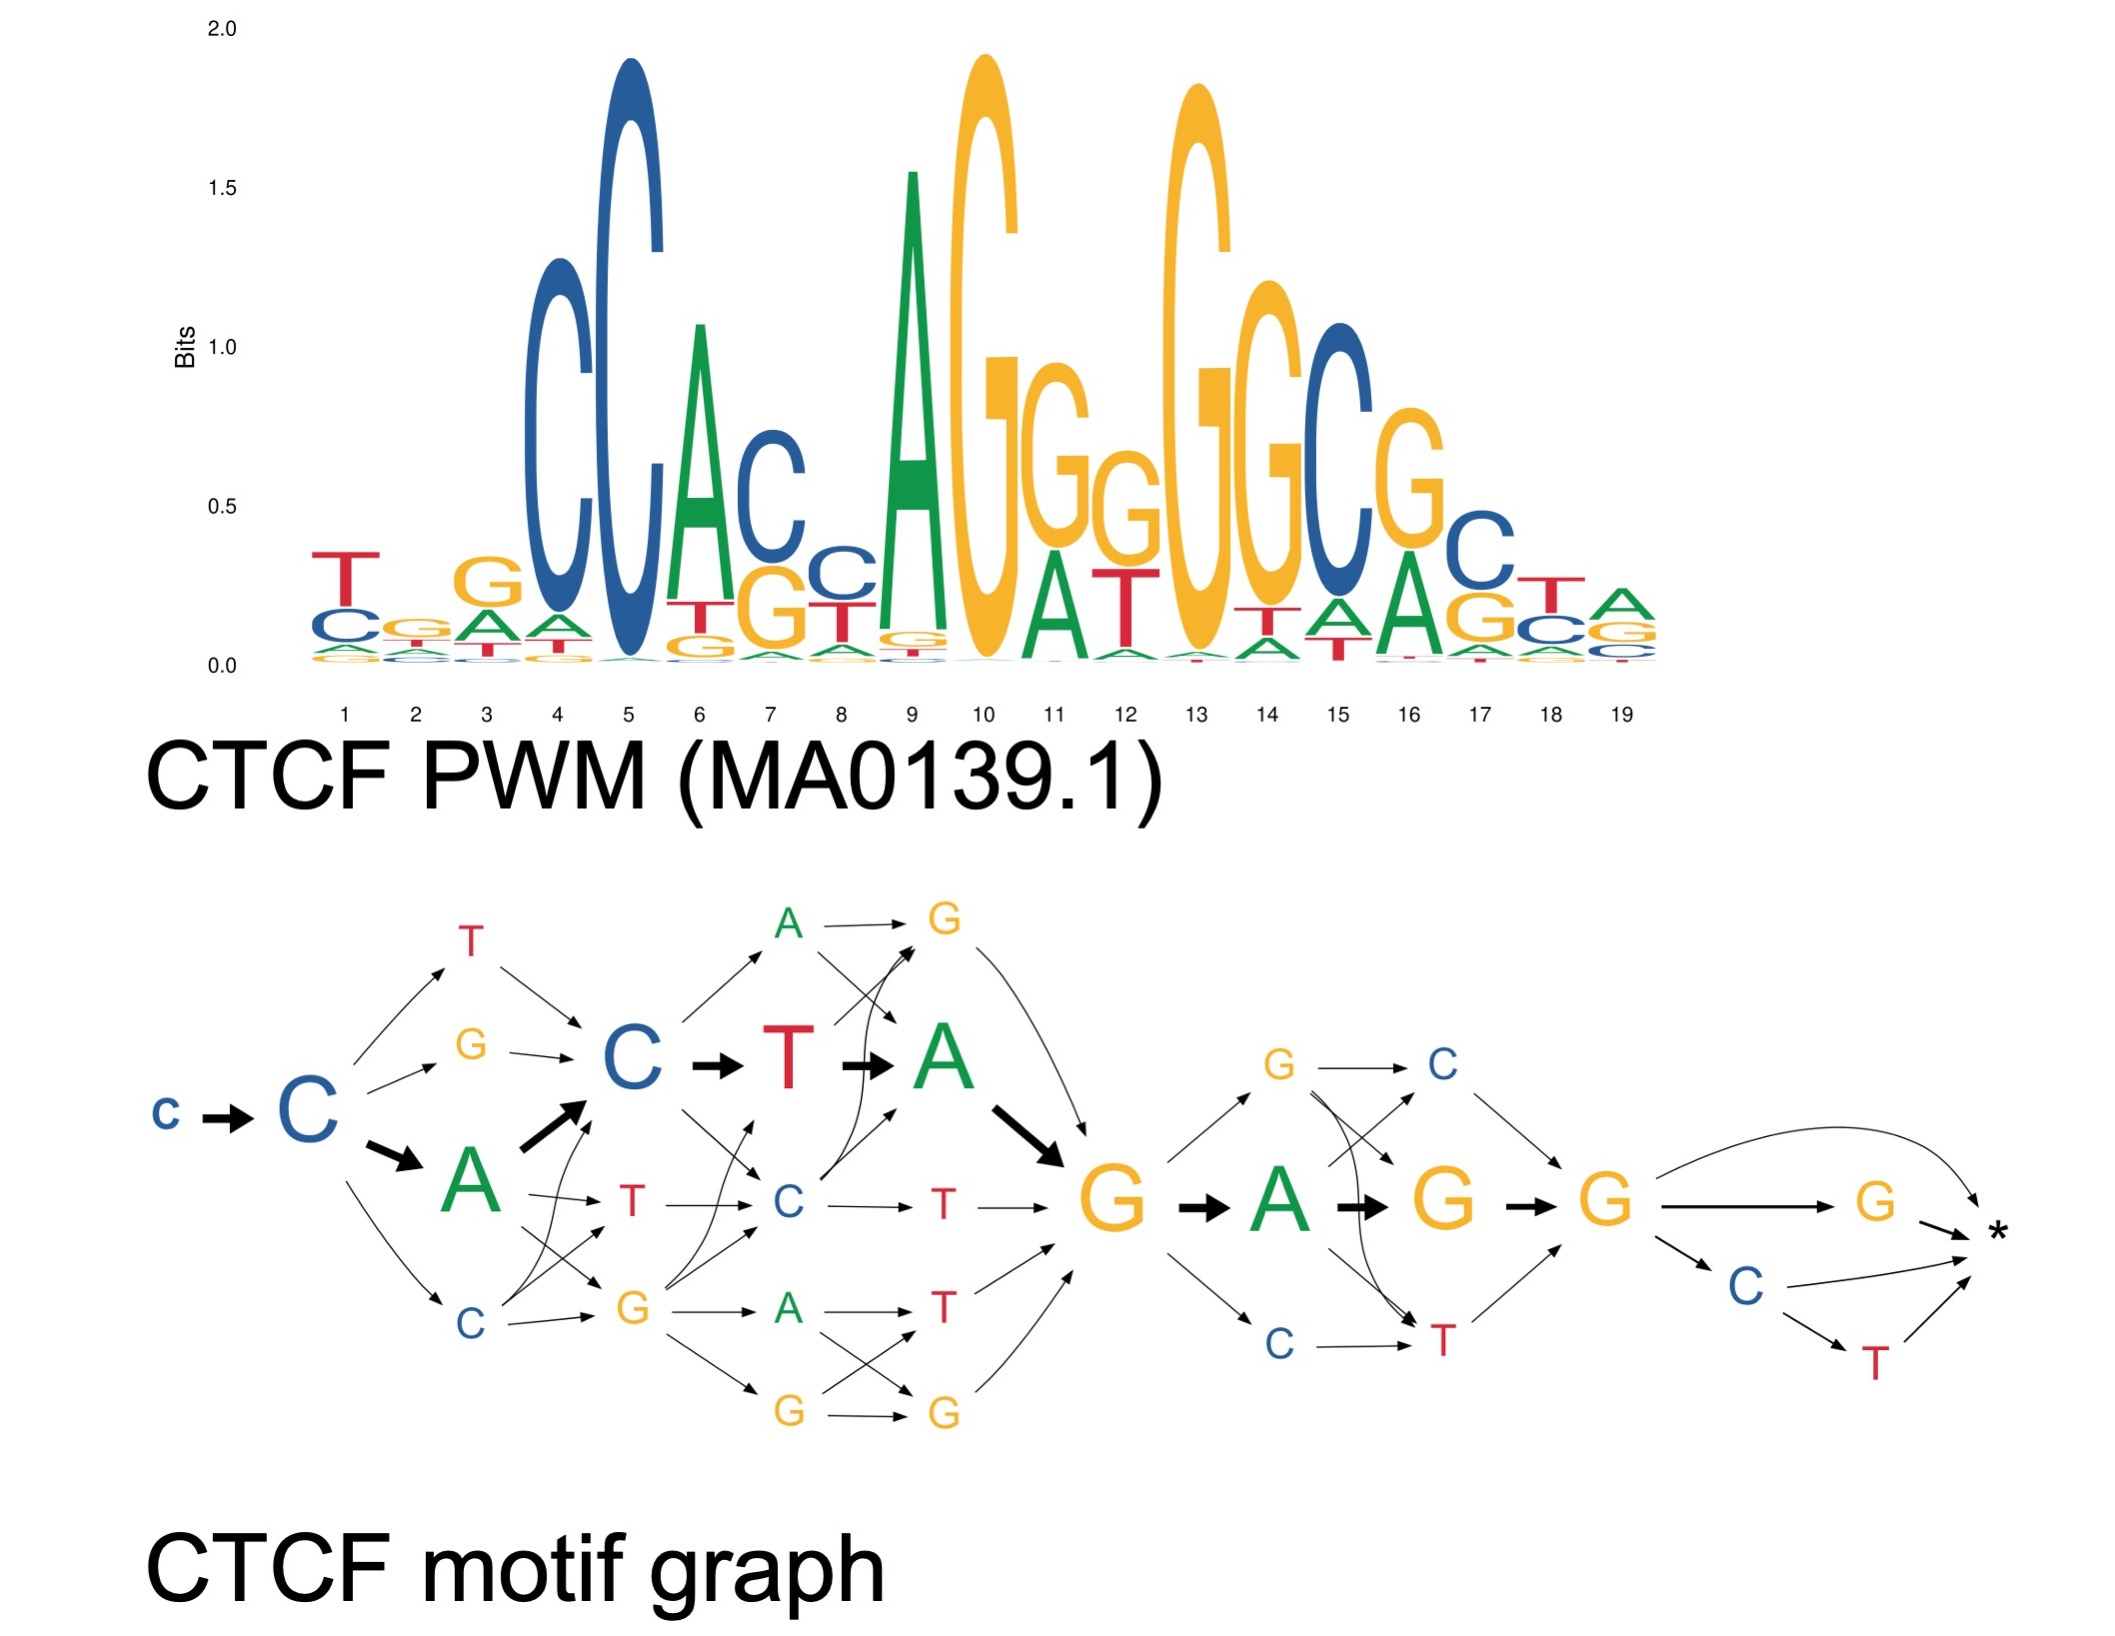
\includegraphics[width=\textwidth]{figures/ctcf_mg.jpg}
	\caption[Comparison between CTCF Motif Graph model and its PWM from the JASPAR database.]{\textbf{Comparison between CTCF MotifGraph model and its PWM from the JASPAR database.} On top the CTCF motif available on JASPAR database (MA0139.1). On the bottom the Motif Graph model trained using 100 $k$-mers obtained from a ChIP-seq experiment trageting CTCF binding site on HepG2 cell line.}
	\label{fig:ctcf_mg}
\end{figure} 
Moreover, such models would better predict the consequences of noncoding variants on TF-DNA binding events, and they could encode variable orders of nucleotide dependencies. Importantly, graph data structures are often interpretable and intuitive. With this aims in mind we developed the Motif Graph, a framework integrating the advantages of \emph{probabilistic graphical models-based} and \emph{SVM-based} motif discovery algorithms, without sacrificing model interpretability. A Motif Graph model $G$ is defined by a set of vertices $V$, a set of edges $E$, and a set of paths $P$. Each vertex $v \in V$ on the graph is labeled with a nucleotide, or mathematically $label(v) \in \{A, C, G, T\}$. Each edge $e \in E$ represents the allowed links between consecutive nucleotides in the TFBS motif. Each path $p \in P$ represents a \emph{haplotype} embedded in $G$, which correspond to one sequence used to train the Motif Graph model. Currently, the model is limited to encode $1$st order dependencies between consecutive nucleotides. However, the model is flexible and accomodate variable length motifs, beside recording the training sequences.
% ---- Motif Graph model construction
\section{Motif Graph model construction}
Motif Graph motif discovery procedure (\textbf{Algorithm \ref{algo:md_mg}}) is constitued of two main steps: $k$-mers prioritization, and graph model training and construction. To prioritize the $k$-mers Motif Graph currently employs the $k$-mer based motif discovery procedure implemented in Gkm-SVM \citep{ghandi2014enhanced}. Therefore, given a positive sequence dataset $S$ and a background dataset $B$, for each $k$-mer of length $k$ in $S$, the algorithm counts the number of matches in $S$ and in $B$, allowing mismatching positions (see \textbf{Section 2.1.2} for further details). Then, a similarity kernel is trained using the recovered $k$-mers frequencies. The trained kernel assigns to each $k$-mer in $S$ and in $B$ a weight proportional to its contribution in defining the foreground or the background dataset. The algorithm then ranks the $k$-mers according to their weight scores. The Motif Graph model is iteratively trained employing a greedy approach, which adds the top ranked $k$-mers to $G$ incrementally, one by one (see \textbf{Algorithm \ref{algo:mt_mg}} for details). Each $k$-mer is aligned to the current $G$ to maximize the number of nucleotides matching the current model. While aligning the $k$-mers to the current Motif Graph model, the algorithm shifts the input $k$-mer on the right and on the left up to a defined offset number of nucleotides. In our experiments with set the offset to $3$. Once built the model, we construct a scoring matrix similar to the widely used $PSSM$. However, our scoring matrix account for $1$st order dependencies between nucleotides, recalling the well-known DWMs (see \textbf{Section 2.1.3} for details). The scoring matrix is used to assign a likelihood score and classify new sequences as potentially bound or not bound by the investigated factor. In other words, the score describes how likely is the scanned sequence to contain a potential binding site. To score a sequence we slide the scoring matrix along the string employing a procedure similar to classical PWM scanning tools like FIMO \citep{grant2011fimo}.
\begin{algorithm}
	\DontPrintSemicolon
	\KwInput{$S$, $B$, $k$}
	\KwOutput{$G$}

	frequencies $\gets$ countFrequencies($S$, $B$, $k$)

	kernel $\gets$ trainKernel(frequencies)

	kmers, weights $\gets$ extractWeights(kernel)

	rankedKmer $\gets$ sort(kmers, weights)

	$G \gets \emptyset$

	\For{kmer in rankedKmers}
	{
		$G \gets$ addKmers($G$, kmer)
	}

	\Return{$G$}
	\caption{\textbf{Motif Graph motif discovery.}}
	\label{algo:md_mg}
\end{algorithm}
\begin{algorithm}
	\DontPrintSemicolon
	\KwInput{$G$, kmer, $i$}
	\KwOutput{$G$}
	
	\If{$i = 1$}
	{
		\Return{$G$}
	}

	\For{$j$ in $1$ to $3$}
	{
		matchesLeftOffset, alignmnetLeft $\gets$ countMatchesLeftOffset($G$, kmer, $j$)
	}

	\For{$j$ in $1$ to $3$}
	{
		matchesRightOffset, alignmnetRight $\gets$ countMatchesRightOffset($G$, kmer, $j$)
	}	
	
	alignment $\gets$ getBestAlignment(matchesLeftOffset, alignmentLeft, matchesRightOffset, alignmentRight)

	$G \gets$ insertKmer($G$, alignment)

	\Return{$G$}
	\caption{\textbf{Motif Graph model training.}}
	\label{algo:mt_mg}
\end{algorithm}
\section{Results}
To test our motif discovery algorithm we obtained $10,000$ ChIP-seq peak sequences from the ENCODE Project database \citep{encode2012integrated} for CTCF and GATA1 Transcription Factors, obtained on the HepG2 and K562 cell lines, respectively. The original ChIP-seq datasets were sorted according to the peaks enrichment score in decreasing order, in order to test our algorithm on reliable peaks. Interestingly, the trained Motif Graph models were closed to the motifs PWM available on the JASPAR database \citep{sandelin2004jaspar} for both CTCF and GATA1 (\textbf{Fig.\ref{fig:ctcf_mg}} and \textbf{Fig.\ref{fig:gata1_mg}}). For both TFs, the Motif Graph models captured the main motif sequence. The main motifs are also enforced by the edge thickness which is proportional to the number of training $k$-mers supporting each $p \in P$.
\begin{figure}
	\centering
	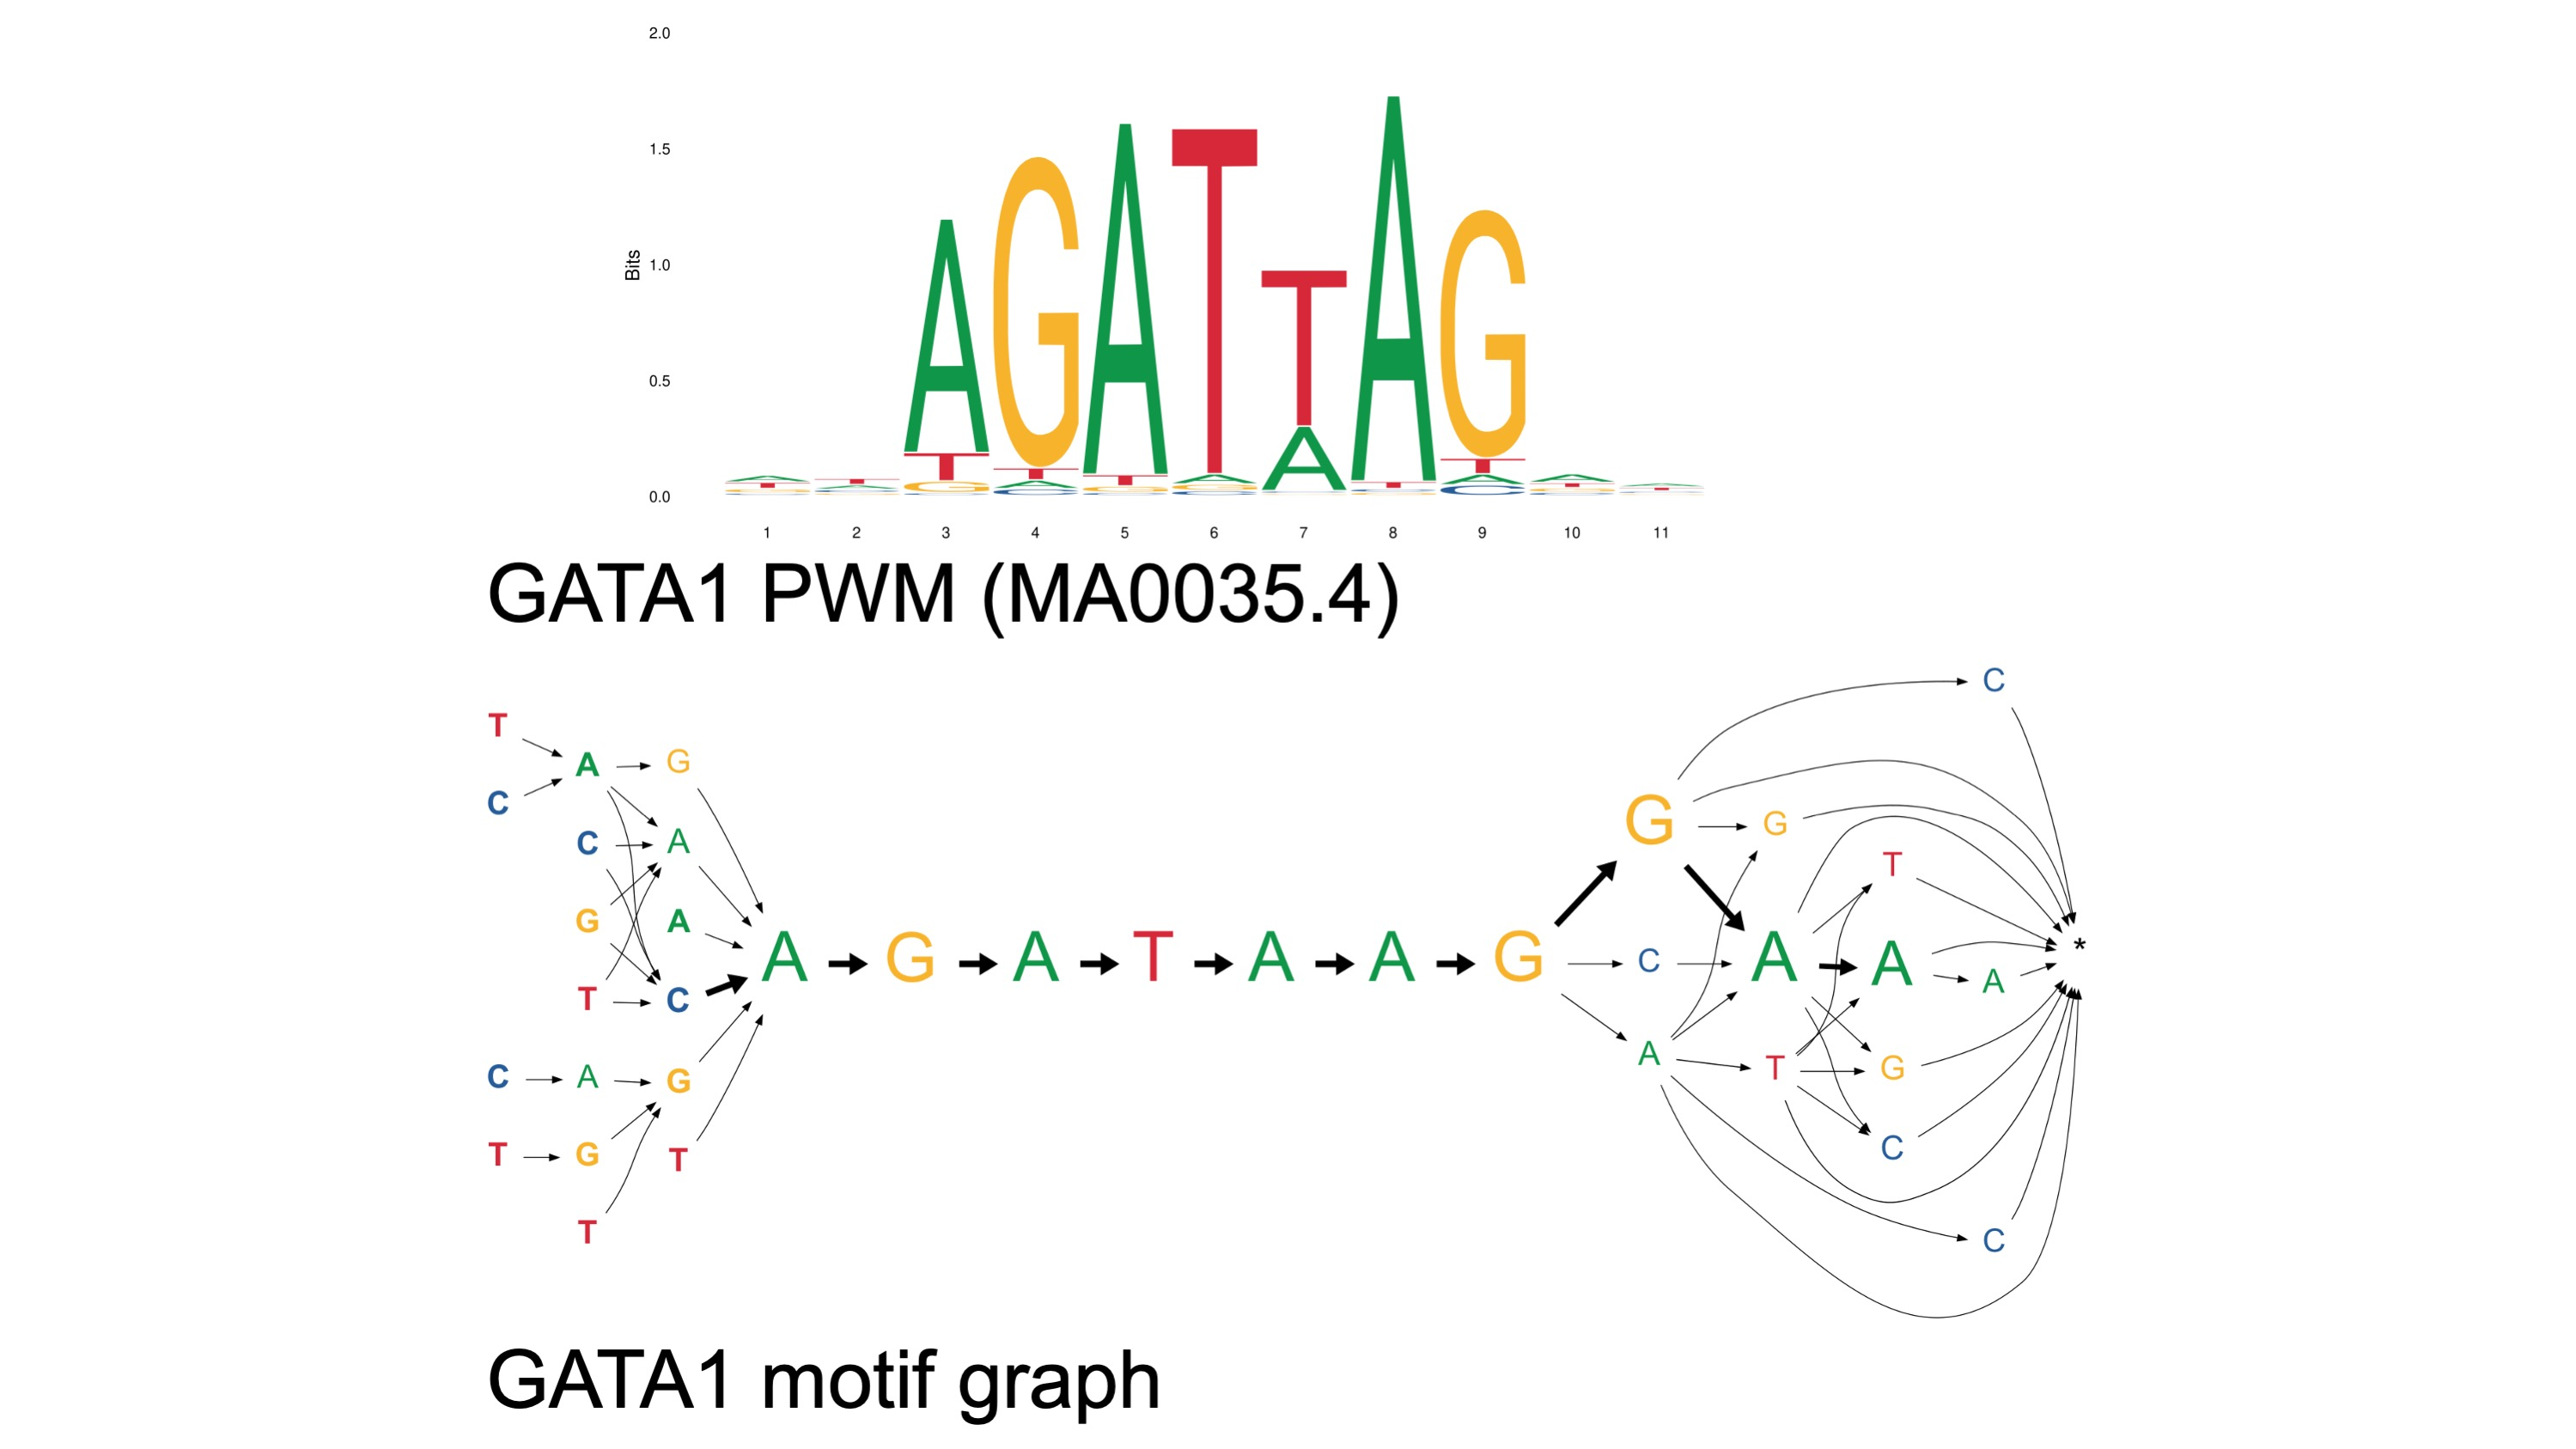
\includegraphics[width=\textwidth]{figures/gata1_mg.jpg}
	\caption[Comparison between GATA1 Motif Graph model and its PWM from the JASPAR database.]{\textbf{Comparison between GATA1 MotifGraph model and its PWM from the JASPAR database.} On top the GATA1 motif available on JASPAR database (MA0035.4). On the bottom the Motif Graph model trained using 100 $k$-mers obtained from a ChIP-seq experiment trageting GATA1 binding site on K562 cell line.}
	\label{fig:gata1_mg}
\end{figure} 
Then, we tested the discriminative performance of both Motif Graph model, with different number of training $k$-mers (\textbf{Fig.\ref{fig:dp_mg}}), to establish the optimal number of training sequences for the CTCF and GATA1 Motif Graph models. To compare the models discriminative performance, we performed a cross-validation experiment using splitting the $S$ and $B$ dataset in training and testing set (75\% and 25\%, respectively). We trained the models with $10$, $50$, $100$, $200$, $350$, $500$, and $750$ $k$-mers. For CTCF the best prformance in terms of both AUC ($0.72$) and F1-score ($0.71$) were obtained training the Motif Graph on $100$ $k$-mers (\textbf{Table \ref{table:ctcf_auc_f1}}). For GATA1 the model returned the best AUC using $200$ $k$-mers ($0.76$), while the best F1-score ($0.70$) was obtained training the model with $100$ sequences (\textbf{Table \ref{table:gata1_auc_f1}}).
\begin{figure}
	\centering
	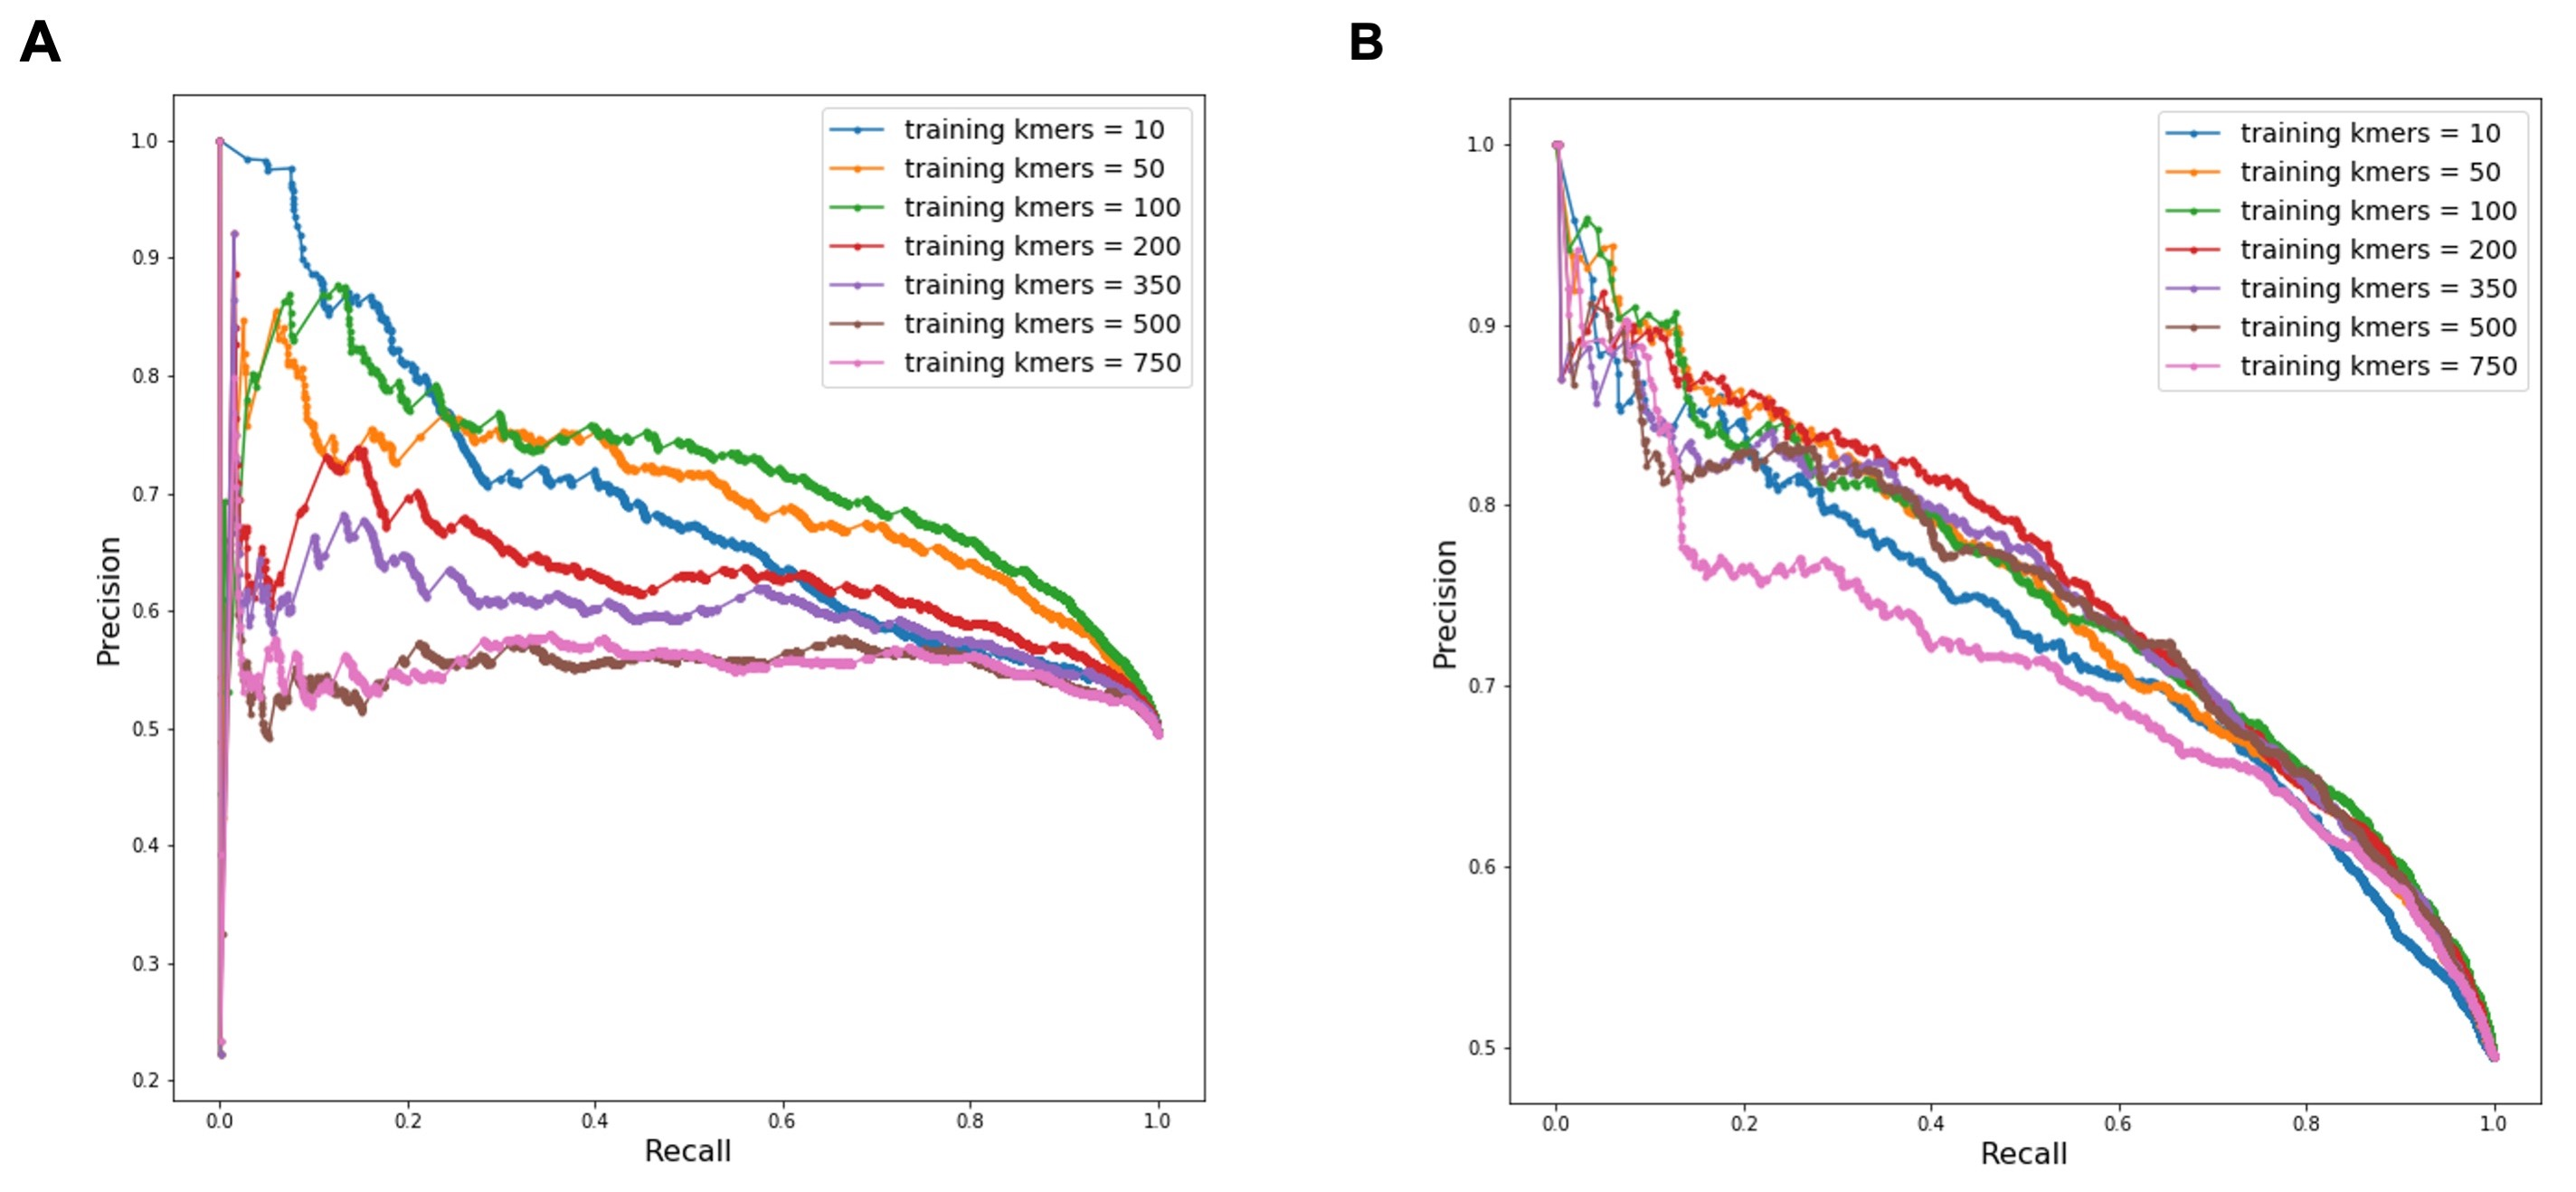
\includegraphics[width=\textwidth]{figures/dp_mg.jpg}
	\caption[Precision-Recall curves obtained varying the number of $k$-mers used to train the Motif Graph models.]{\textbf{Precision-Recall curves obtained varying the number of $k$-mers used to train the Motif Graph models.} To establish the number of training $k$-mers returning the best discriminative performance we computed the Precision-Recall curves of different Motif Graph models trained using 10, 50, 100, 200, 350, 500, and 750 $k$-mers on \textbf{(A)} CTCF and \textbf{(B)} GATA1}
	\label{fig:dp_mg}
\end{figure} 
\begin{table}
	\centering
	\begin{tabular}{|p{3cm}|p{1.cm}|p{1.cm}|p{1.cm}|p{1.cm}|p{1.cm}|p{1.cm}|p{1.cm}|}
		\hline
		\textbf{Training $k$-mers}& \textbf{$10$}& \textbf{$50$}& \textbf{$100$}& \textbf{$200$}& \textbf{$350$}& \textbf{$500$}& \textbf{$750$} \\
		\hline
		\textbf{AUC}& $0.69$& $0.69$& $0.72$& $0.63$& $0.60$& $0.55$& $0.55$\\
		\hline
		\textbf{F1-score}& $0.62$& $0.69$& $0.71$& $0.65$& $0.62$& $0.57$& $0.56$\\
		\hline
	\end{tabular}
	\caption[CTCF Motif Graph model AUC and F1-scores values with different number of training $k$-mers.]{\textbf{CTCF Motif Graph model AUC and F1-scores values with different number of training $k$-mers.}}
	\label{table:ctcf_auc_f1}
\end{table}
\begin{table}
	\centering
	\begin{tabular}{|p{3cm}|p{1.cm}|p{1.cm}|p{1.cm}|p{1.cm}|p{1.cm}|p{1.cm}|p{1.cm}|}
		\hline
		\textbf{Training $k$-mers}& \textbf{$10$}& \textbf{$50$}& \textbf{$100$}& \textbf{$200$}& \textbf{$350$}& \textbf{$500$}& \textbf{$750$} \\
		\hline
		\textbf{AUC}& $0.73$& $0.75$& $0.75$& $0.76$& $0.74$& $0.74$& $0.71$\\
		\hline
		\textbf{F1-score}& $0.68$& $0.68$& $0.70$& $0.69$& $0.70$& $0.69$& $0.67$\\
		\hline
	\end{tabular}
	\caption[GATA1 Motif Graph model AUC and F1-scores values with different number of training $k$-mers.]{\textbf{GATA1 Motif Graph model AUC and F1-scores values with different number of training $k$-mers.}}
	\label{table:gata1_auc_f1}
\end{table}
Then, we compared the Motif Graph models discriminative performance against the corresponding PWM and DWM models, recovered from JASPAR \citep{sandelin2004jaspar} and HOCOMOCO \citep{kulakovskiy2016hocomoco} databases, respectively. For CTCF, both the PWM and the DWM models returned better predictive performance than our model (\textbf{Fig.\ref{fig:dp_mg_pwm_dwm} (A)}). On the other hand, on GATA1 data our model showed better performance than PWMs, but still performed worse than DWMs (\textbf{Fig.\ref{fig:dp_mg_pwm_dwm} (B)}).
\begin{figure}
	\centering
	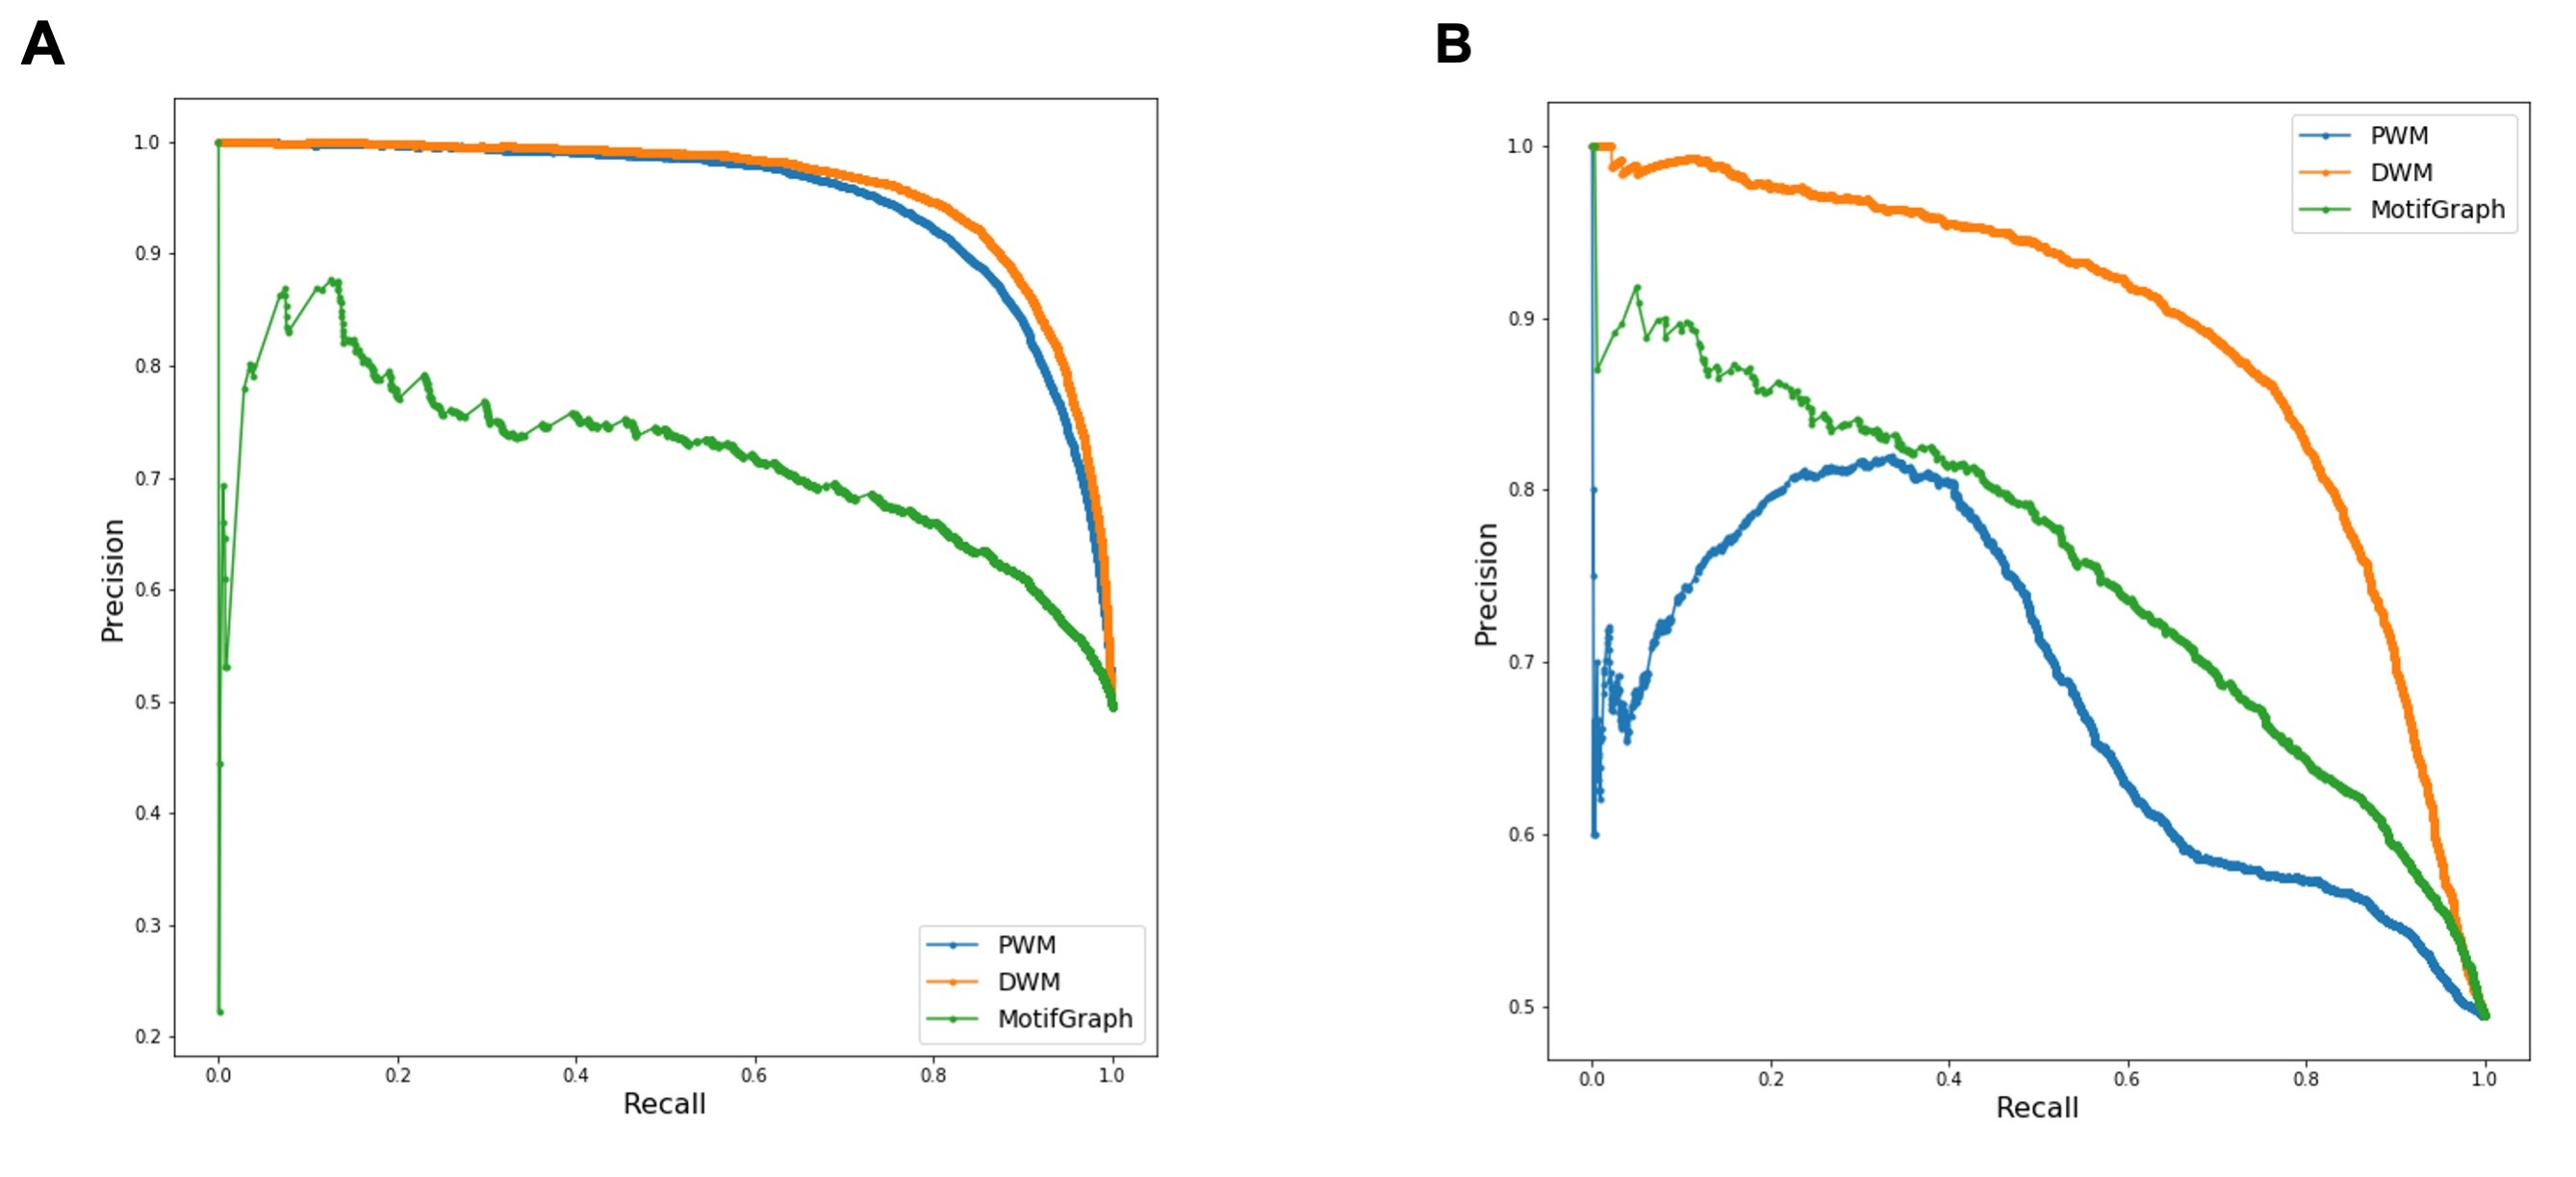
\includegraphics[width=\textwidth]{figures/dp_mg_pwm_dwm.jpg}
	\caption[Comparing Motif Graph, PWM, and DWM Precision-Recall curves.]{\textbf{Comparing Motif Graph, PWM, and DWM Precision-Recall curves.} We compared the discriminative power of the Motif Graph models against that of PWMs and DWMs for both \textbf{(A)} CTCF and \textbf{(B)} GATA1.}
	\label{fig:dp_mg_pwm_dwm}
\end{figure} 
% ------- Variant effects prediction on Transcription Factor Binding Sites
\mychapter{5}{Variant effects prediction on Transcription Factor Binding Sites}
Several studies showed that genetic variants can significantly impact TF-DNA binding events \citep{de2006regulatory,weinhold2014genome,guo2018mutation}. Genome-wide association studies (GWASs) uncovered thousands of genetic variants (SNPs), associated with complex human traits, located in noncoding regions of the genome. Most of these variants are located within functional regulatory elements, like enhancers \citep{maurano2012systematic}. Therefore, misregulations in gene expression may be mediated by SNPs modulating TF-DNA interactions. Such variants may perturb TF-DNA binding sequences, potentially changing the downstream gene expression \citep{deplancke2016genetics}. Importantly, mutations altering TFBS can occur in haplotypes conserved within a population of individuals \citep{kasowski2010variation}, resulting in population specific TFBS. Similarly, cell-type genetic variability can create cell-type specific TF target sequences. Therefore, the development of software designed to predict the potential effects of genetic variation on TFBS specificity accounting for haplotype- and cell-type specific mutations becomes fundamental to increase our knowledge about the cell mechanisms governing gene expression. To this aim, we developed two tools predicting mutations effects on TFBS in haplotypes and different cell-types. GRAFIMO \citep{tognon2021grafimo} is a variant- and haplotype-aware motif scanning tool searching potential occurrences of known TF motifs on genome graphs \citep{paten2017genome}. Briefly, genome graphs are graph-based data structures, where nodes correspond to DNA sequences and edges describe allowed links between successive sequences. Paths through the graph, which may be labelled (such as in the case of a reference genome), correspond to haplotypes belonging to different genomes \citep{siren2020haplotype} (\textbf{Fig.\ref{fig:vg}}).
Variants like SNPs and indels form bubbles in the graph, where diverging paths through the graph are anchored by a common start and end sequence on the reference
[138]. 
\begin{figure}
	\centering
	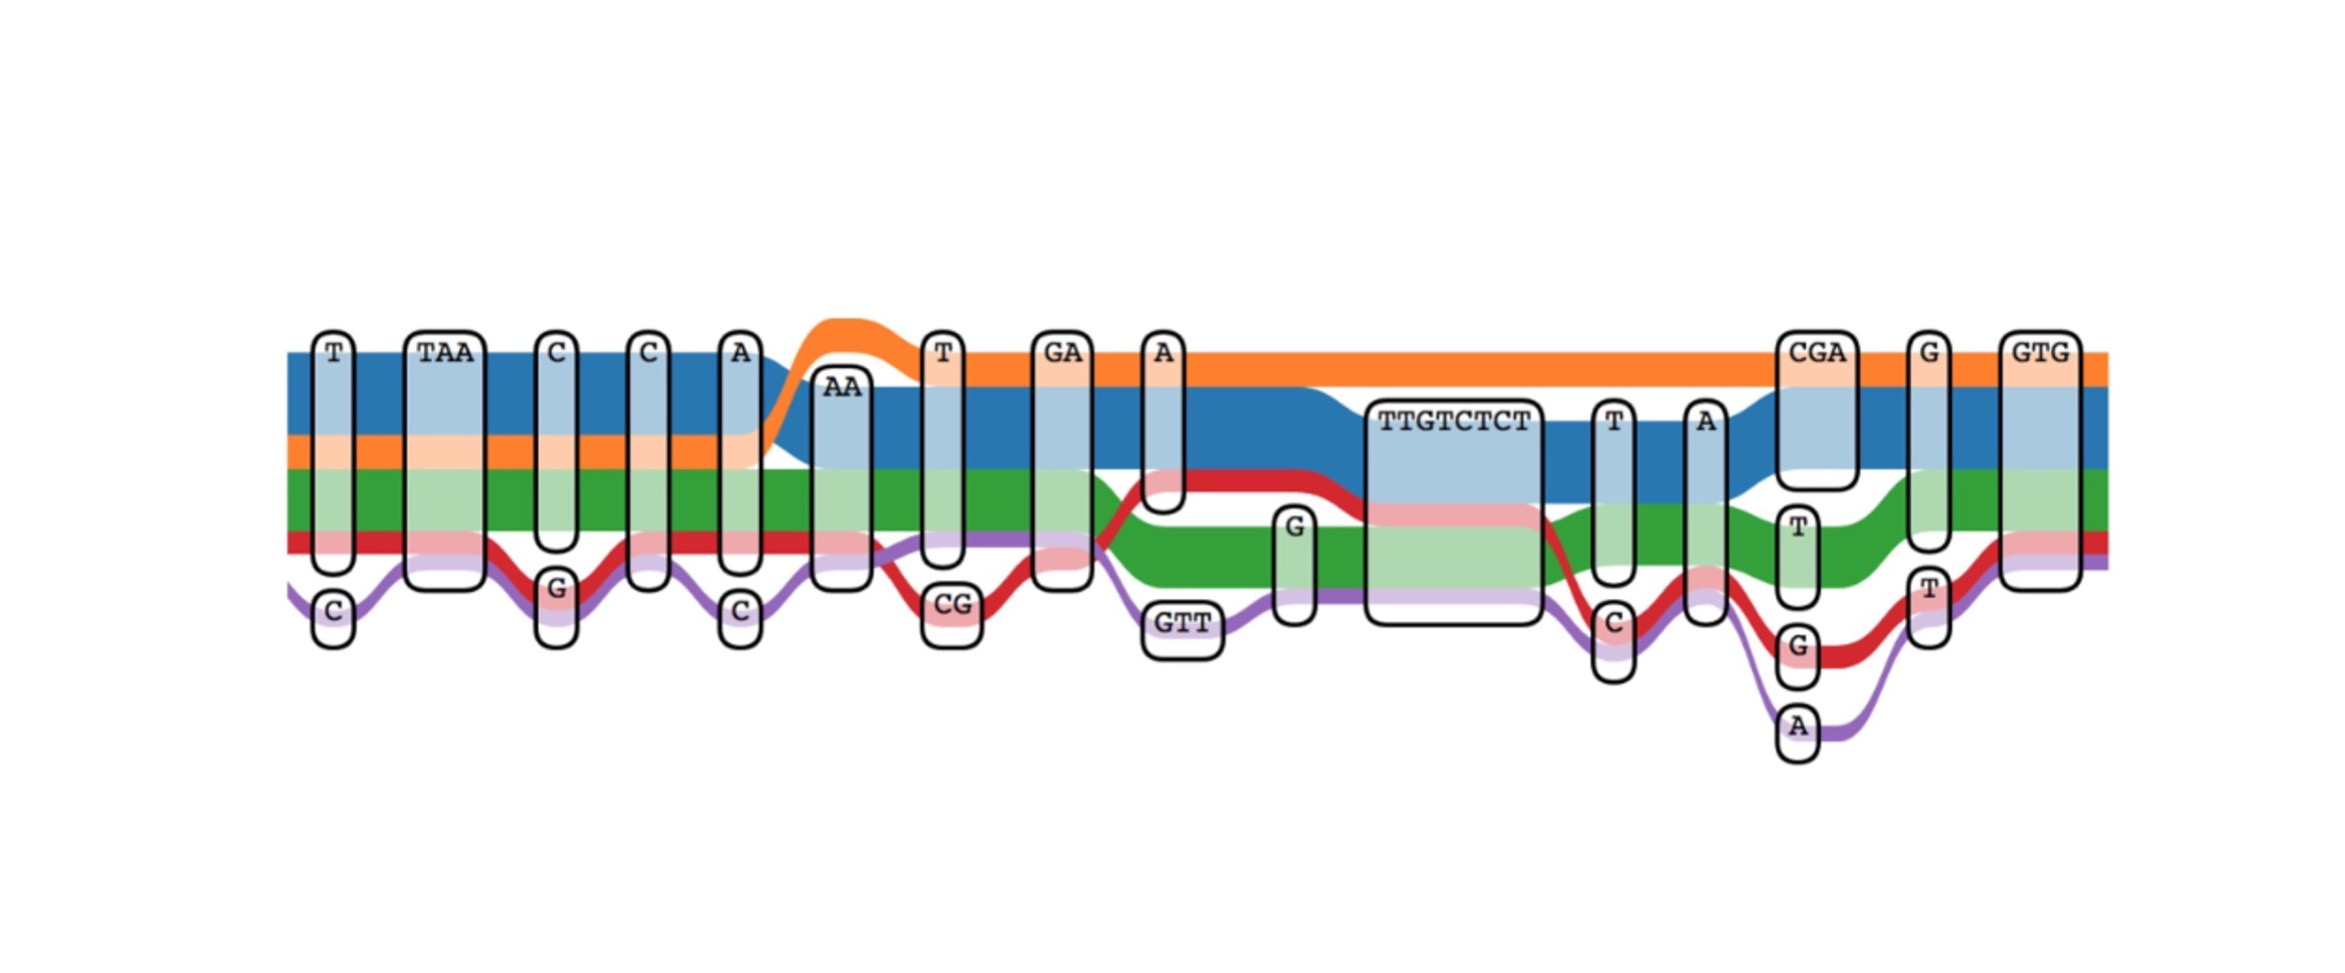
\includegraphics[width=\textwidth]{figures/vg.jpg}
	\caption[Genome Graphs data structure visualization]{\textbf{Genome Graphs data structure visualization.}  Each color corresponds to a path in the graph. Each path represents the genomic sequences of one of the individual genomes encoded in the Genome Graph structure.}
	\label{fig:vg}
\end{figure} 
MotifRaptor \citep{yao2021motif} investigates the impact of genetic variants on TF, exploiting cell-type specific information regarding chromatin accessibility and gene expression. While the original MotifRaptor used PWM models to assess genetic variants effects, we extended the framework to integrate $k$-mer-based motif models (see \textbf{Section 2.1.3} for details), which provide more reliable predictions.
% ---- GRAFIMO
\section{GRAFIMO}
GRAFIMO (GRAph-based Finding of Individual Motif Occurrences) \citep{tognon2021grafimo} is a command-line tool to scan known TF DNA motifs represented as PWMs in genome variation graphs (VGs) \citep{garrison2018variation}, a scalable and efficient implement of genome graph framework. GRAFIMO extends the standard PWM scanning procedure by considering variations and alternative haplotypes encoded in a VG. Using GRAFIMO on a VG based on individuals from the 1000 Genomes project \citep{siva20081000} we recover several potential binding sites that are enhanced, weakened or missed when scanning only the reference genome, and which could constitute individual-specific binding events. During the last decade, several methods have been developed to search TFBS on linear reference genomes, such as FIMO \citep{grant2011fimo} and MOODS \citep{korhonen2009moods} or to account for SNPs and short indels such as is-rSNP, TRAP and atSNP \citep{macintyre2010rsnp,thomas2011transcription,zuo2015atsnp}, however these tools do not account for individual haplotypes nor provide summary on the frequency of these events in a population. We observed that several CTCF motif occurrences are found only in non-reference haplotypes, therefore a consistent number of potential motif occurrences are potentially lost when scanning only the reference sequence (\textbf{Fig.\ref{fig:grafimo1} (A)}). 
\begin{figure}
	\centering
	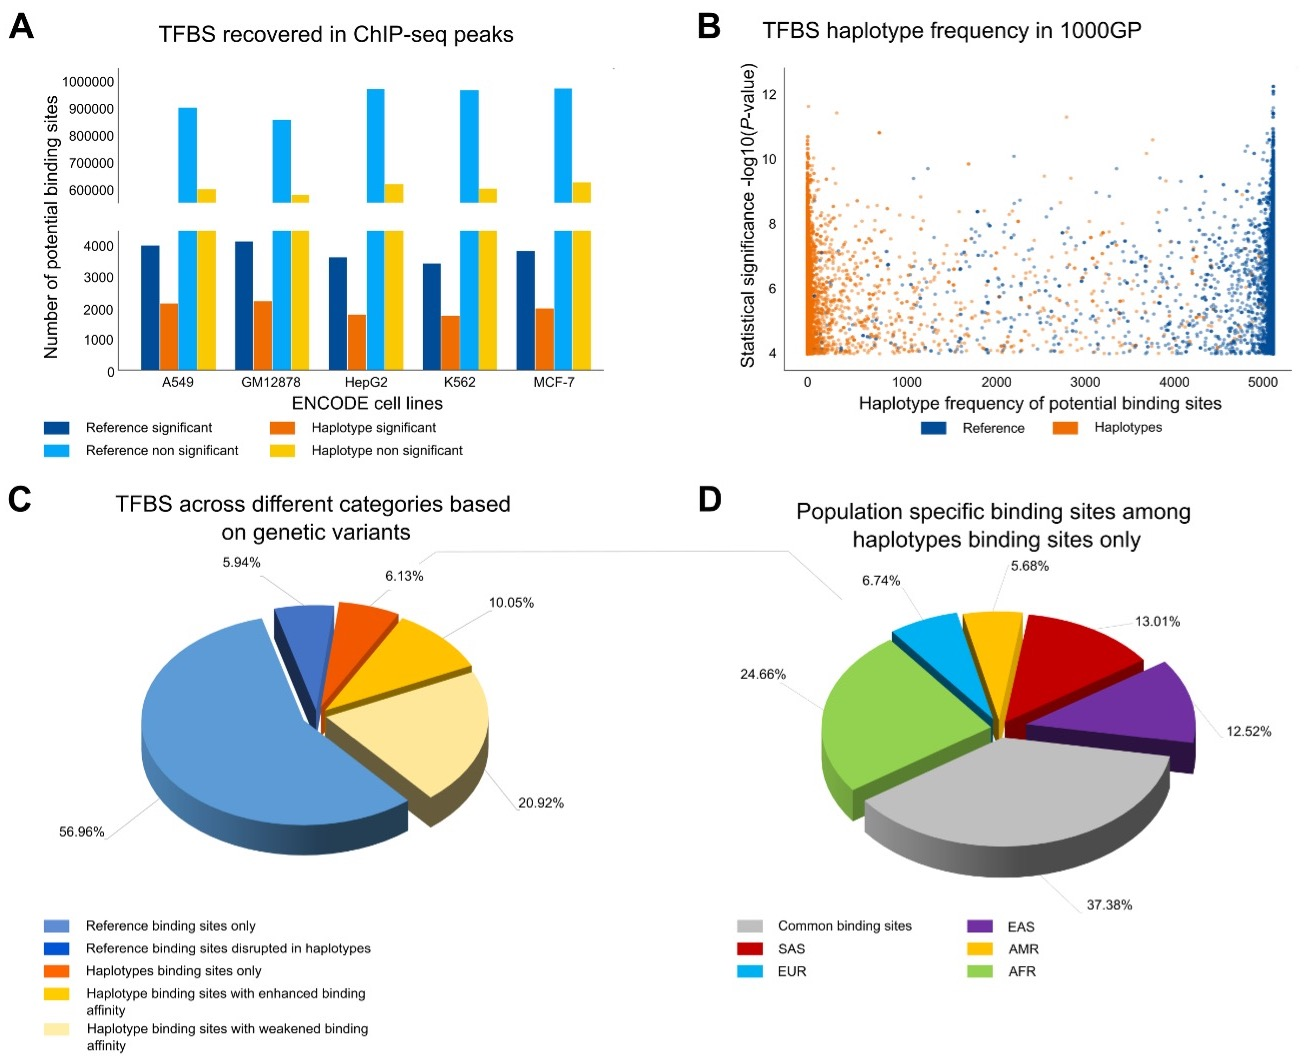
\includegraphics[width=\textwidth]{figures/grafimo1.jpg}
	\caption[Searching CTCF motif on VG with GRAFIMO provides an insight on how genetic variation affects putative
binding sites]{\textbf{Searching CTCF motif on VG with GRAFIMO provides an insight on how genetic variation affects putative
binding sites. (A)} Potential CTCF occurrences statistically significant (P-value < 1e-4) and non-significant found in the
reference and in the haplotype sequences found with GRAFIMO oh hg38 1000GP VG. (\textbf{B)} Statistical significance of
retrieved potential CTCF motif occurrences and frequency of the corresponding haplotypes embedded in the VG. \textbf{(C)}
Percentage of statistically significant CTCF potential binding sites found only in the reference genome or alternative
haplotypes and with modulated binding scores based on 1000GP genetic variants \textbf{(D)} Percentage of population specific and
common (shared by two or more populations) potential CTCF binding sites present on individual haplotypes.}
	\label{fig:grafimo1}
\end{figure} 
Moreover, we found several potential CTCF occurrences with high statistical significance occurring in rare haplotypes, which could modulate gene expression in those subjects (\textbf{Fig.\ref{fig:grafimo1} (B)}). We also investigated how often regulatory mutations disrupt, create or modulate TFBS binding affinity. Interestingly, we observed that many TFBS can be found only on individual
haplotypes. Moreover, ~ 6\% of TFBS are disrupted (do not survive the ss threshold) by the presence of genetic variants, while ~30\% of potential CTCF TFBS are still significant in non-reference haplotypes, but with enhanced or weakened ba score (\textbf{Fig.\ref{fig:grafimo1} (C)}). We also observed that several putative non-reference TFBS are population-specific (\textbf{Fig.\ref{fig:grafimo1} (D)}). Among the unique CTCF motif occurrences found only on non-reference haplotypes in CTCF ChIP-seq peaks we uncovered one
TFBS (chr19:506,910-506,929) that clearly illustrates the danger of only using reference genomes for motif scanning. Within this region we recovered a heterozygous SNP that overlaps (position 10 of the CTCF matrix) and significantly modulates the binding affinity of this TFBS. In fact, by inspecting the ChIP-seq reads (experiment ENCSR000DZN, GM12878 cell line), we observed a clear allelic imbalance towards the alternative allele \texttt{G} (70.59\% of reads) with respect to the reference allele \texttt{A} (29.41\% of reads). This allelic imbalance is not observed in the reads used as control (experiment code ENCSR000EYX) (\textbf{Fig.\ref{fig:grafimo2}}). Taken together these results highlight the importance of considering non-reference genome data when searching for potential TFBS or to characterize their potential activity in a population of individuals.
\begin{figure}
	\centering
	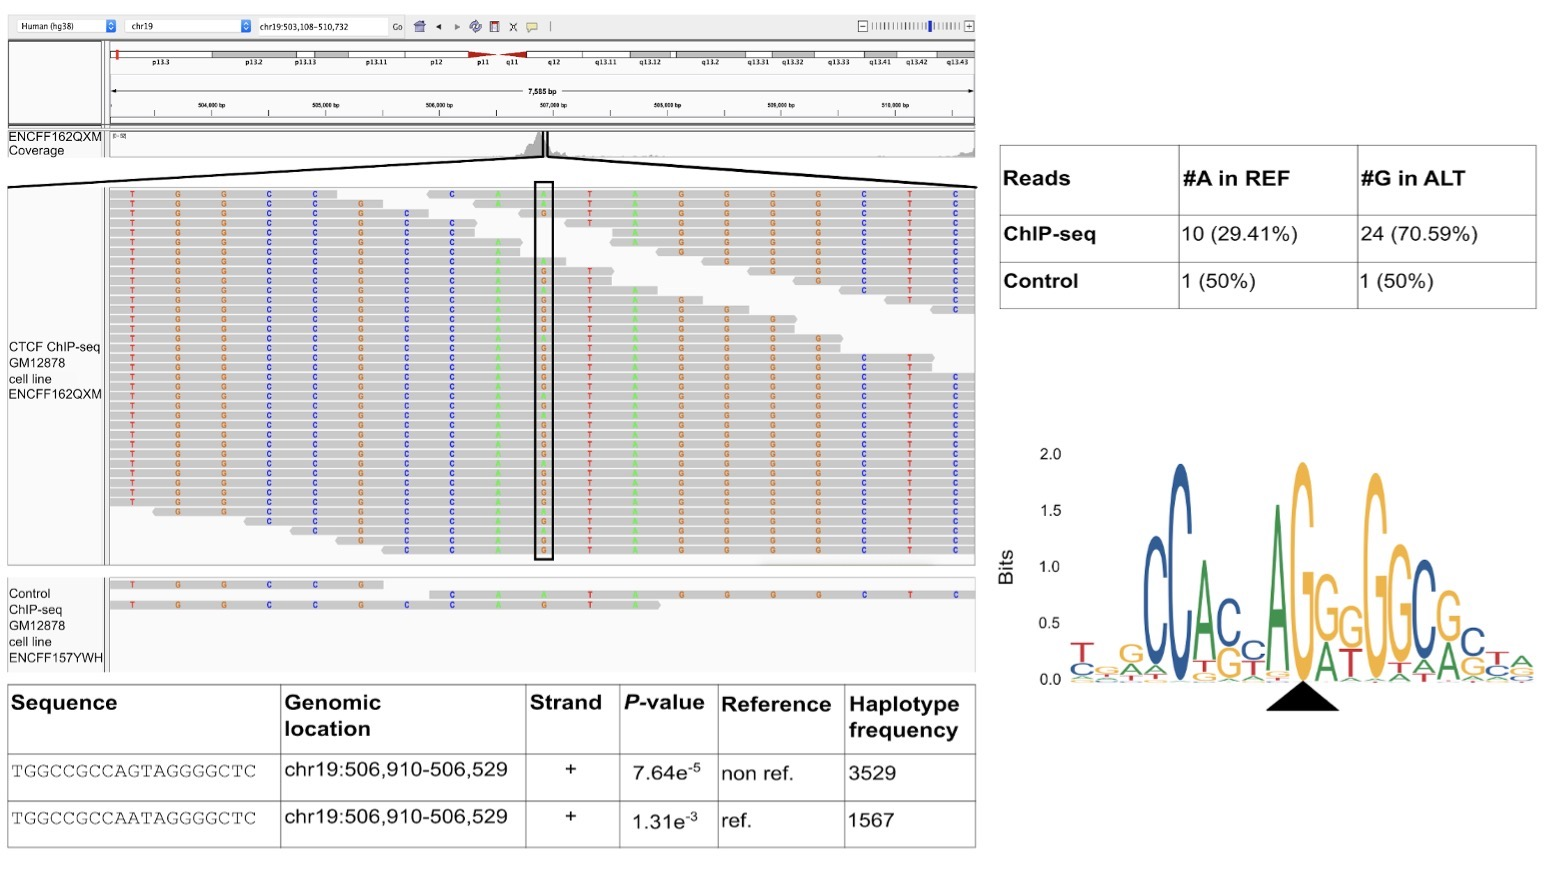
\includegraphics[width=\textwidth]{figures/grafimo2.jpg}
	\caption[Considering genomic variation, GRAFIMO captures more potential binding events]{\textbf{Considering genomic variation, GRAFIMO captures more potential binding events.} GRAFIMO reports a potential CTCF binding site at chr19:506,910-506,929 found only in haplotype sequences, searching the motif in ChIP-seq peaks called on cell line GM12878 (experiment code ENCSR000DZN). The reads used to call for ChIP-seq peaks (ENCFF162QXM) show an allelic imbalance at position 10 of the motif sequence towards the alternative allele \texttt{G}, instead of the reference allele \texttt{A}. The imbalance is captured by GRAFIMO which reports the sequence presenting \texttt{G} at position 10 (found in the haplotypes), while the potential TFBS on the reference carrying an \texttt{A} is not reported as statistically significant ($P$-value > 1e-4). CTCF motif logo shows that the \texttt{G} is the dominant nucleotide in position 10.}
	\label{fig:grafimo2}
\end{figure} 
% ---- MotifRaptor2
\section{MotifRaptor2}
Several studies showed that genetic variants can enhance or disrupt TF-DNA binding affinities. Moreover, most of the SNPs ($\sim90\%$) associated to common diseases and complex phenotypical traits thorugh GWAS analyses have been located within REs, such as enhancers or promoters. MotifRaptor exploits cell-type specific data, like chromatin accessibility and gene expression, to predict the impact of SNPs prioritized via GWAS on TFBS sequence and the corresponding TF-DNA interactions. MotifRaptor workflow is currently constitued of three steps (\textbf{Fig.\ref{fig:motifraptor1}}). (i) TCharacterize important cell-types through the enrichment of the phenotype associated SNPs in open chromatin regions. (ii) Search TFBS whose binding potential is significantly modulated by the previously prioritized variants, in the investigated cell-types. (iii) Identify and visualize individual TF-SNP modulation events. 
\begin{figure}
	\centering
	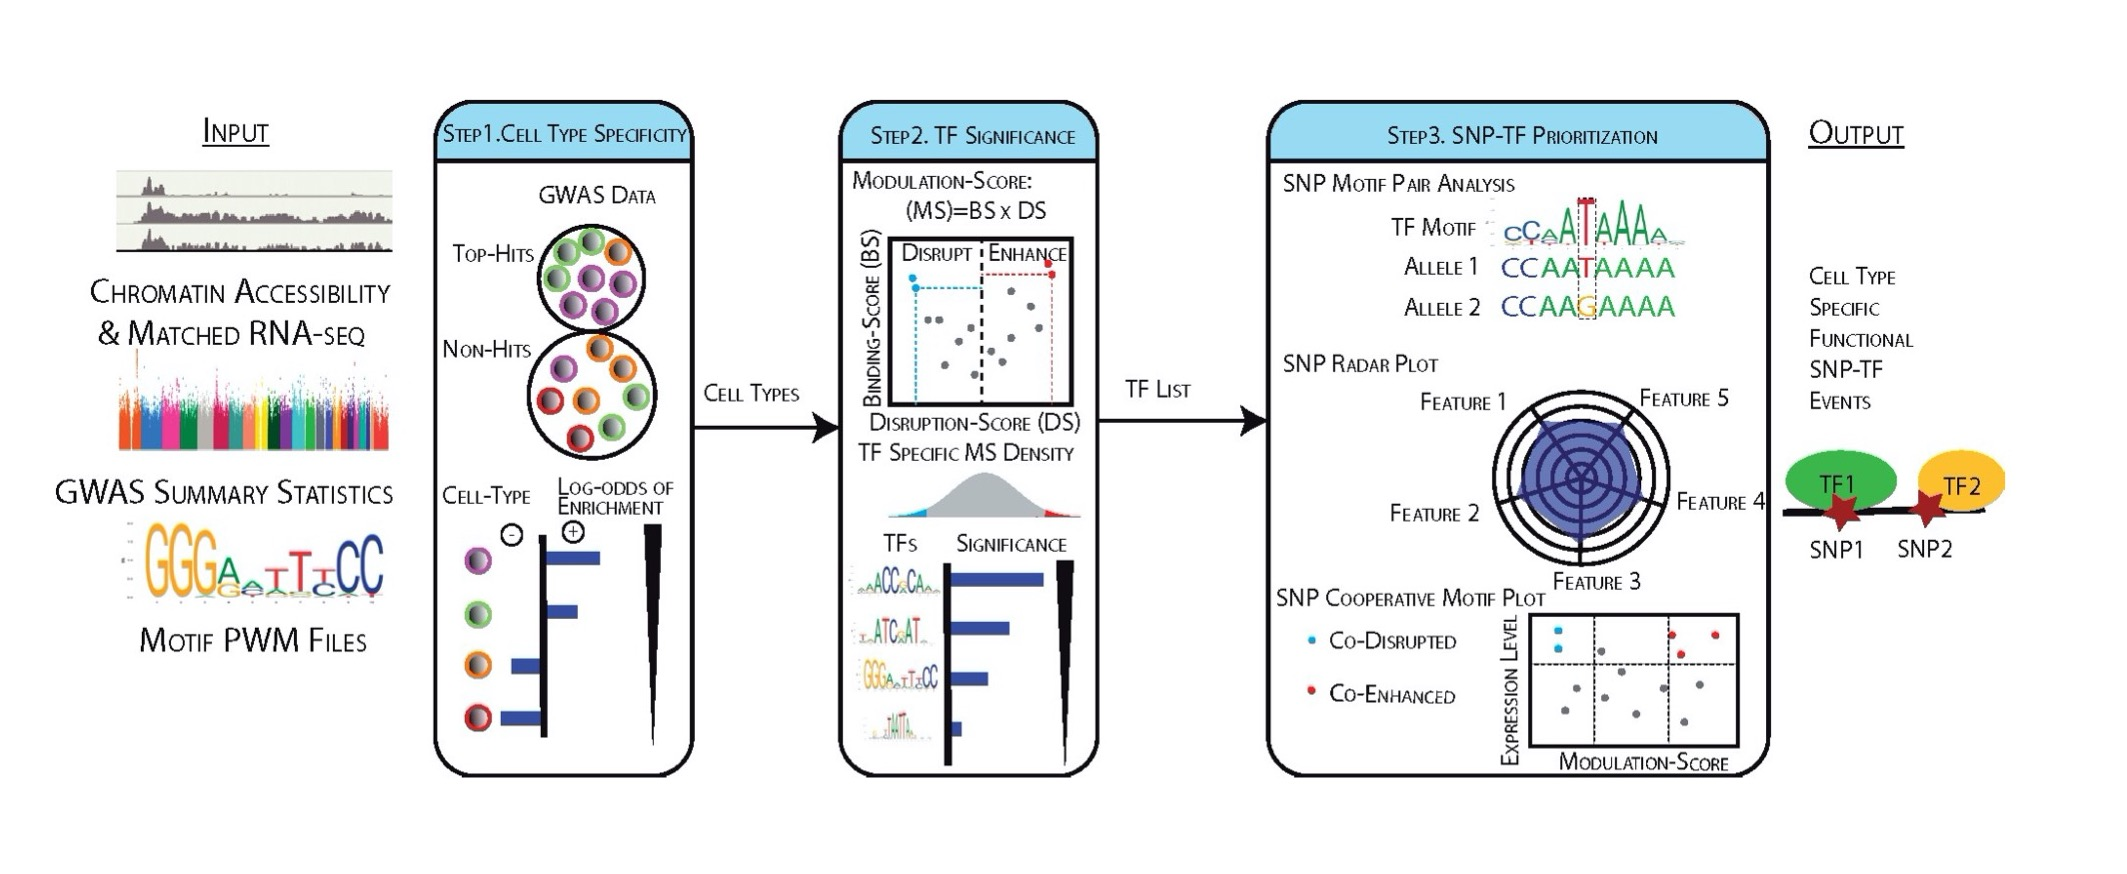
\includegraphics[width=\textwidth]{figures/motifraptor1.jpg}
	\caption[MotifRaptor analysis workflow]{\textbf{MotifRaptor analysis workflow.} Three steps are performed: (1) characterize
relevant cell types based on the enrichment of phenotype associated SNPs in chromatin accessible
sites, (2) find TFs with binding sites that are significantly modulated by genetic variants in these
cell types and (3) identify and visualize individual TF-SNP regulation events}
	\label{fig:motifraptor1}
\end{figure} 
The original MotifRaptor employed TFBS PWM models to predict SNP impact on the binding sites of the investigated factor. However, PWMs have several limitations, like the assumption of independence between neighboring and non-neighboring nucleotides within TF target sites, and often they require large amount of training data to return reliable models \citep{zhao2011quantitative} (see \textbf{Section 2.1.3} for details). $K$-mer-based motif models address some of PWMs' limitations. (i) $K$-mers are features that are either present or not in the training dataset, therefore, the resulting models do not require large amount of training data. (ii) $K$-mers capture $k$th order dependencies between neighboring nucleotides. Therefore, we extended the MotifRaptor analysis to consider $k$-mer-based motif models to assess the impact of genetic variants on TFBS. With this aim we integrated Gkm-SVM analysis pipeline in MotifRaptor framework, to compute sequence scores reflecting SNPs impact on binding sites. We tested MotifRaptor2 by predicting how NFKB1, RUNX3 and STAT1 binding landscapes are affected by genetic variation, considering SNPs linked to rheumatoid arthritis trait. The $k$-mer based models for the investigated TFs were obtained using Gkm-SVM on ChIP-seq peakssequences from the ENCODE Project database. Interestingly, we observed that $k$-mer-based motif models show a higher discriminative power than PWM when identifying bound and unbound sequences (ChIP-seq peak and random sequences, respectively) (\textbf{Fig.\ref{fig:motifraptor2}}).
\begin{figure}
	\centering
	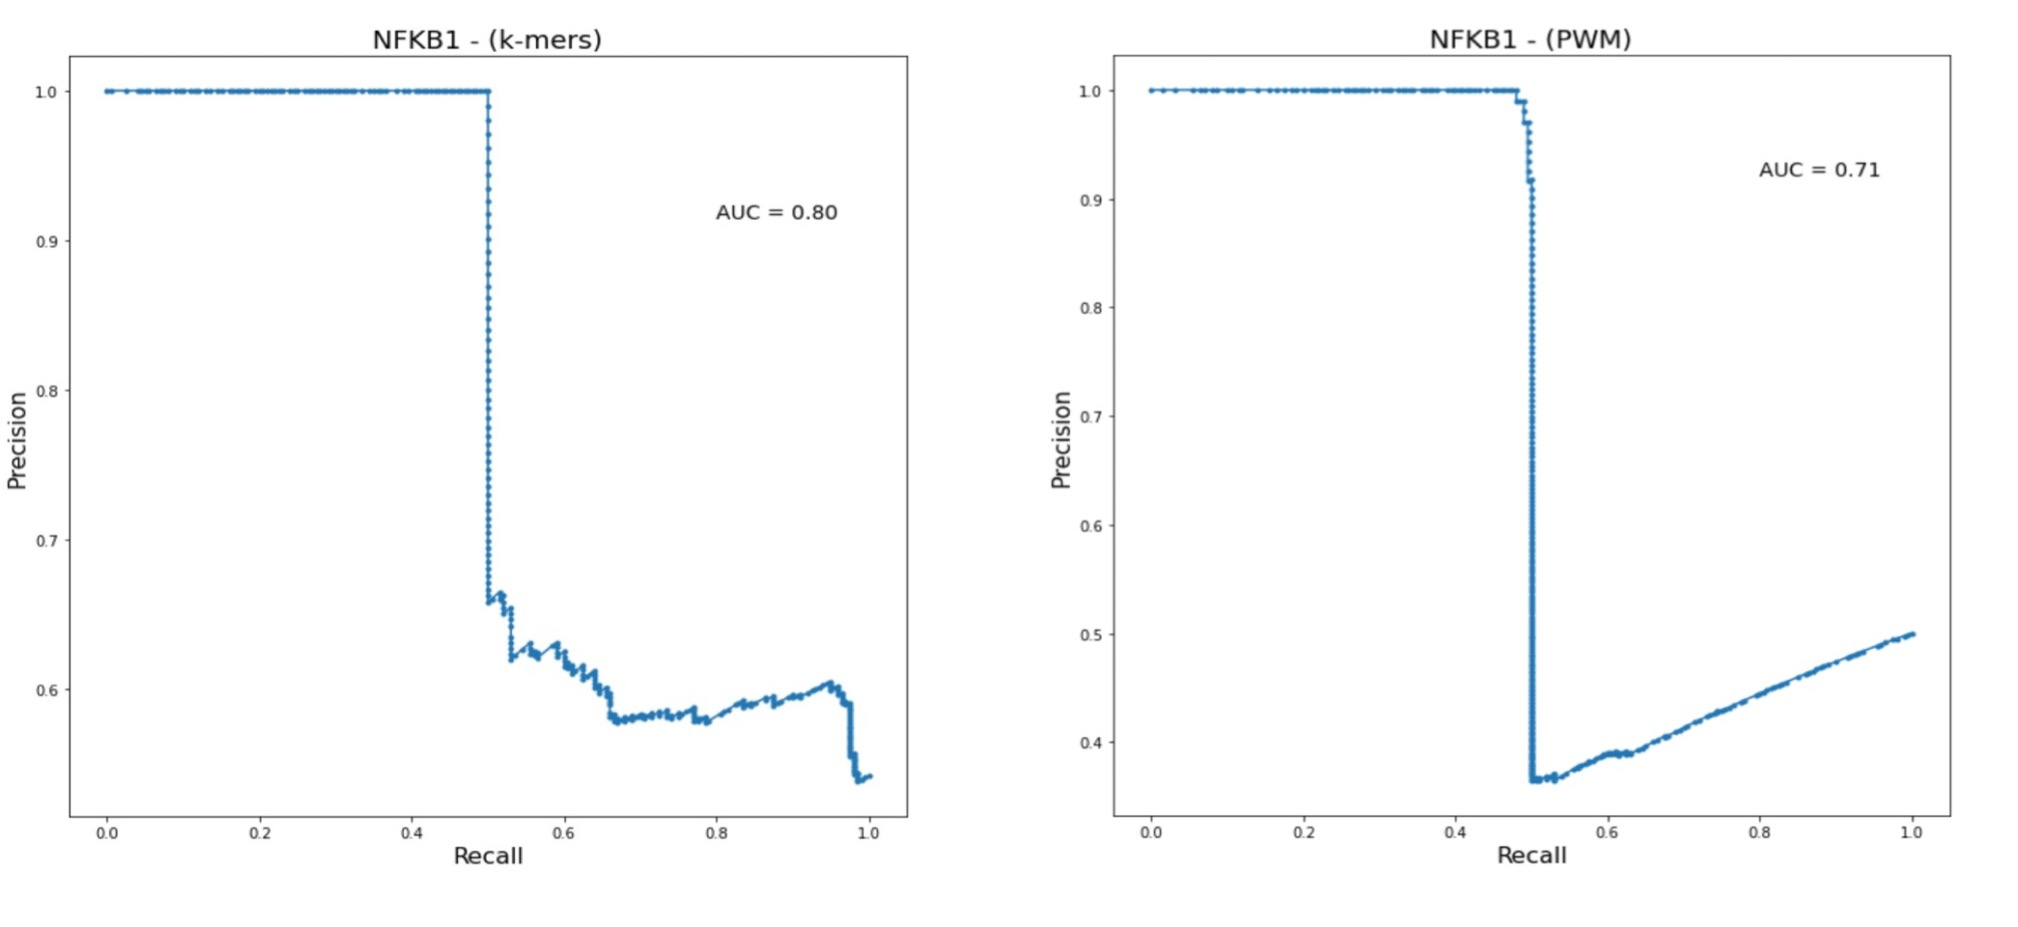
\includegraphics[width=\textwidth]{figures/motifraptor2.jpg}
	\caption[Precision-Recall curves for NFKB1 models ($k$-mers and PWM) and AUC]{\textbf{Precision-Recall curves for NFKB1 models ($k$-mers and PWM) and AUC.}}
	\label{fig:motifraptor2}
\end{figure} 
Therefore, MotifRaptor2 is a promising tool to produce reliable predictions regarding genetic variants impact on transcription factors binding landscapes.
% ------ CRISPR off-targets
\mychapter{6}{CRISPR off-targets}
CRISPR gene editing \citep{cong2013multiplex} enabled the genetic engineering of the genomes of living organisms. CRISPR provides a simple and programmable platform coupling the binding to genomic target sequences with diverse effector proteins restricted by protospacer adjacent motif (PAM) sequences. By delivering the Cas9 nuclease complexed with a synthetic guide RNA (gRNA) into a cell, CRISPR provides a simple and programmable platform to modify the genomic sequence at a desired location, potentially allowing the removal or addition of genes \emph{in vivo}. Importantly, CRISPR offers unprecedented opportunities to develop novel therapies by introducing targeted genetic or epigenetic modifications to the genomic regions of interest. CRISPR-Cas9 offers high fidelity and simple construction and  its specificity depends on two factors: (i) the target sequence and (ii) the PAM sequence. The target sequence is 20 bp long as part of each CRISPR locus in the gRNA array \citep{ran2013genome}. Typically, crRNA has multiple unique targets. Cas9 selects the genomic location by pairing the gRNA with its complementary sequence on the host DNA. Since the gRNA sequence is not part of the Cas9 complex, it can be designed independently to target specific genomic locations \citep{bialk2015regulation}. To exploit the exonucleasic function Cas9 recognize its PAM sequences. PAMs are very short nonspecific sequences, occurring in several locations along the genome \citep{ran2013genome}. Once assembled the required sequences, Cas9 finds the targets on the genome, guided by the gRNA. The Cas9 nuclease opens both genomic strands of the target sequence to introduce novel modifications in it. Cas9 works in two main methods: (i) knock-in, and (ii) knock-out mutations (\textbf{Fig.\ref{fig:crispr}}). In knock-in, homology directed repair (HDR) employs  DNA sequences similar to the targets to repair the breaks in the genome caused by Cas9 exonucleasic actions, using exogenous DNA as repairing template. Importantly, this method relies on periodic and isolated damaged spots in the target sites to start the DNA repair operations. In knock-out, mutations in the DNA inserted by Cas9 result in the repair of breaks through nonhomologous end joining (NHEJ). DNA repair via NHEJ often results in random insertions and deletions in the target sequence, which may disrupt, enhance, or alter the function of the target site.
\begin{figure}
	\centering
	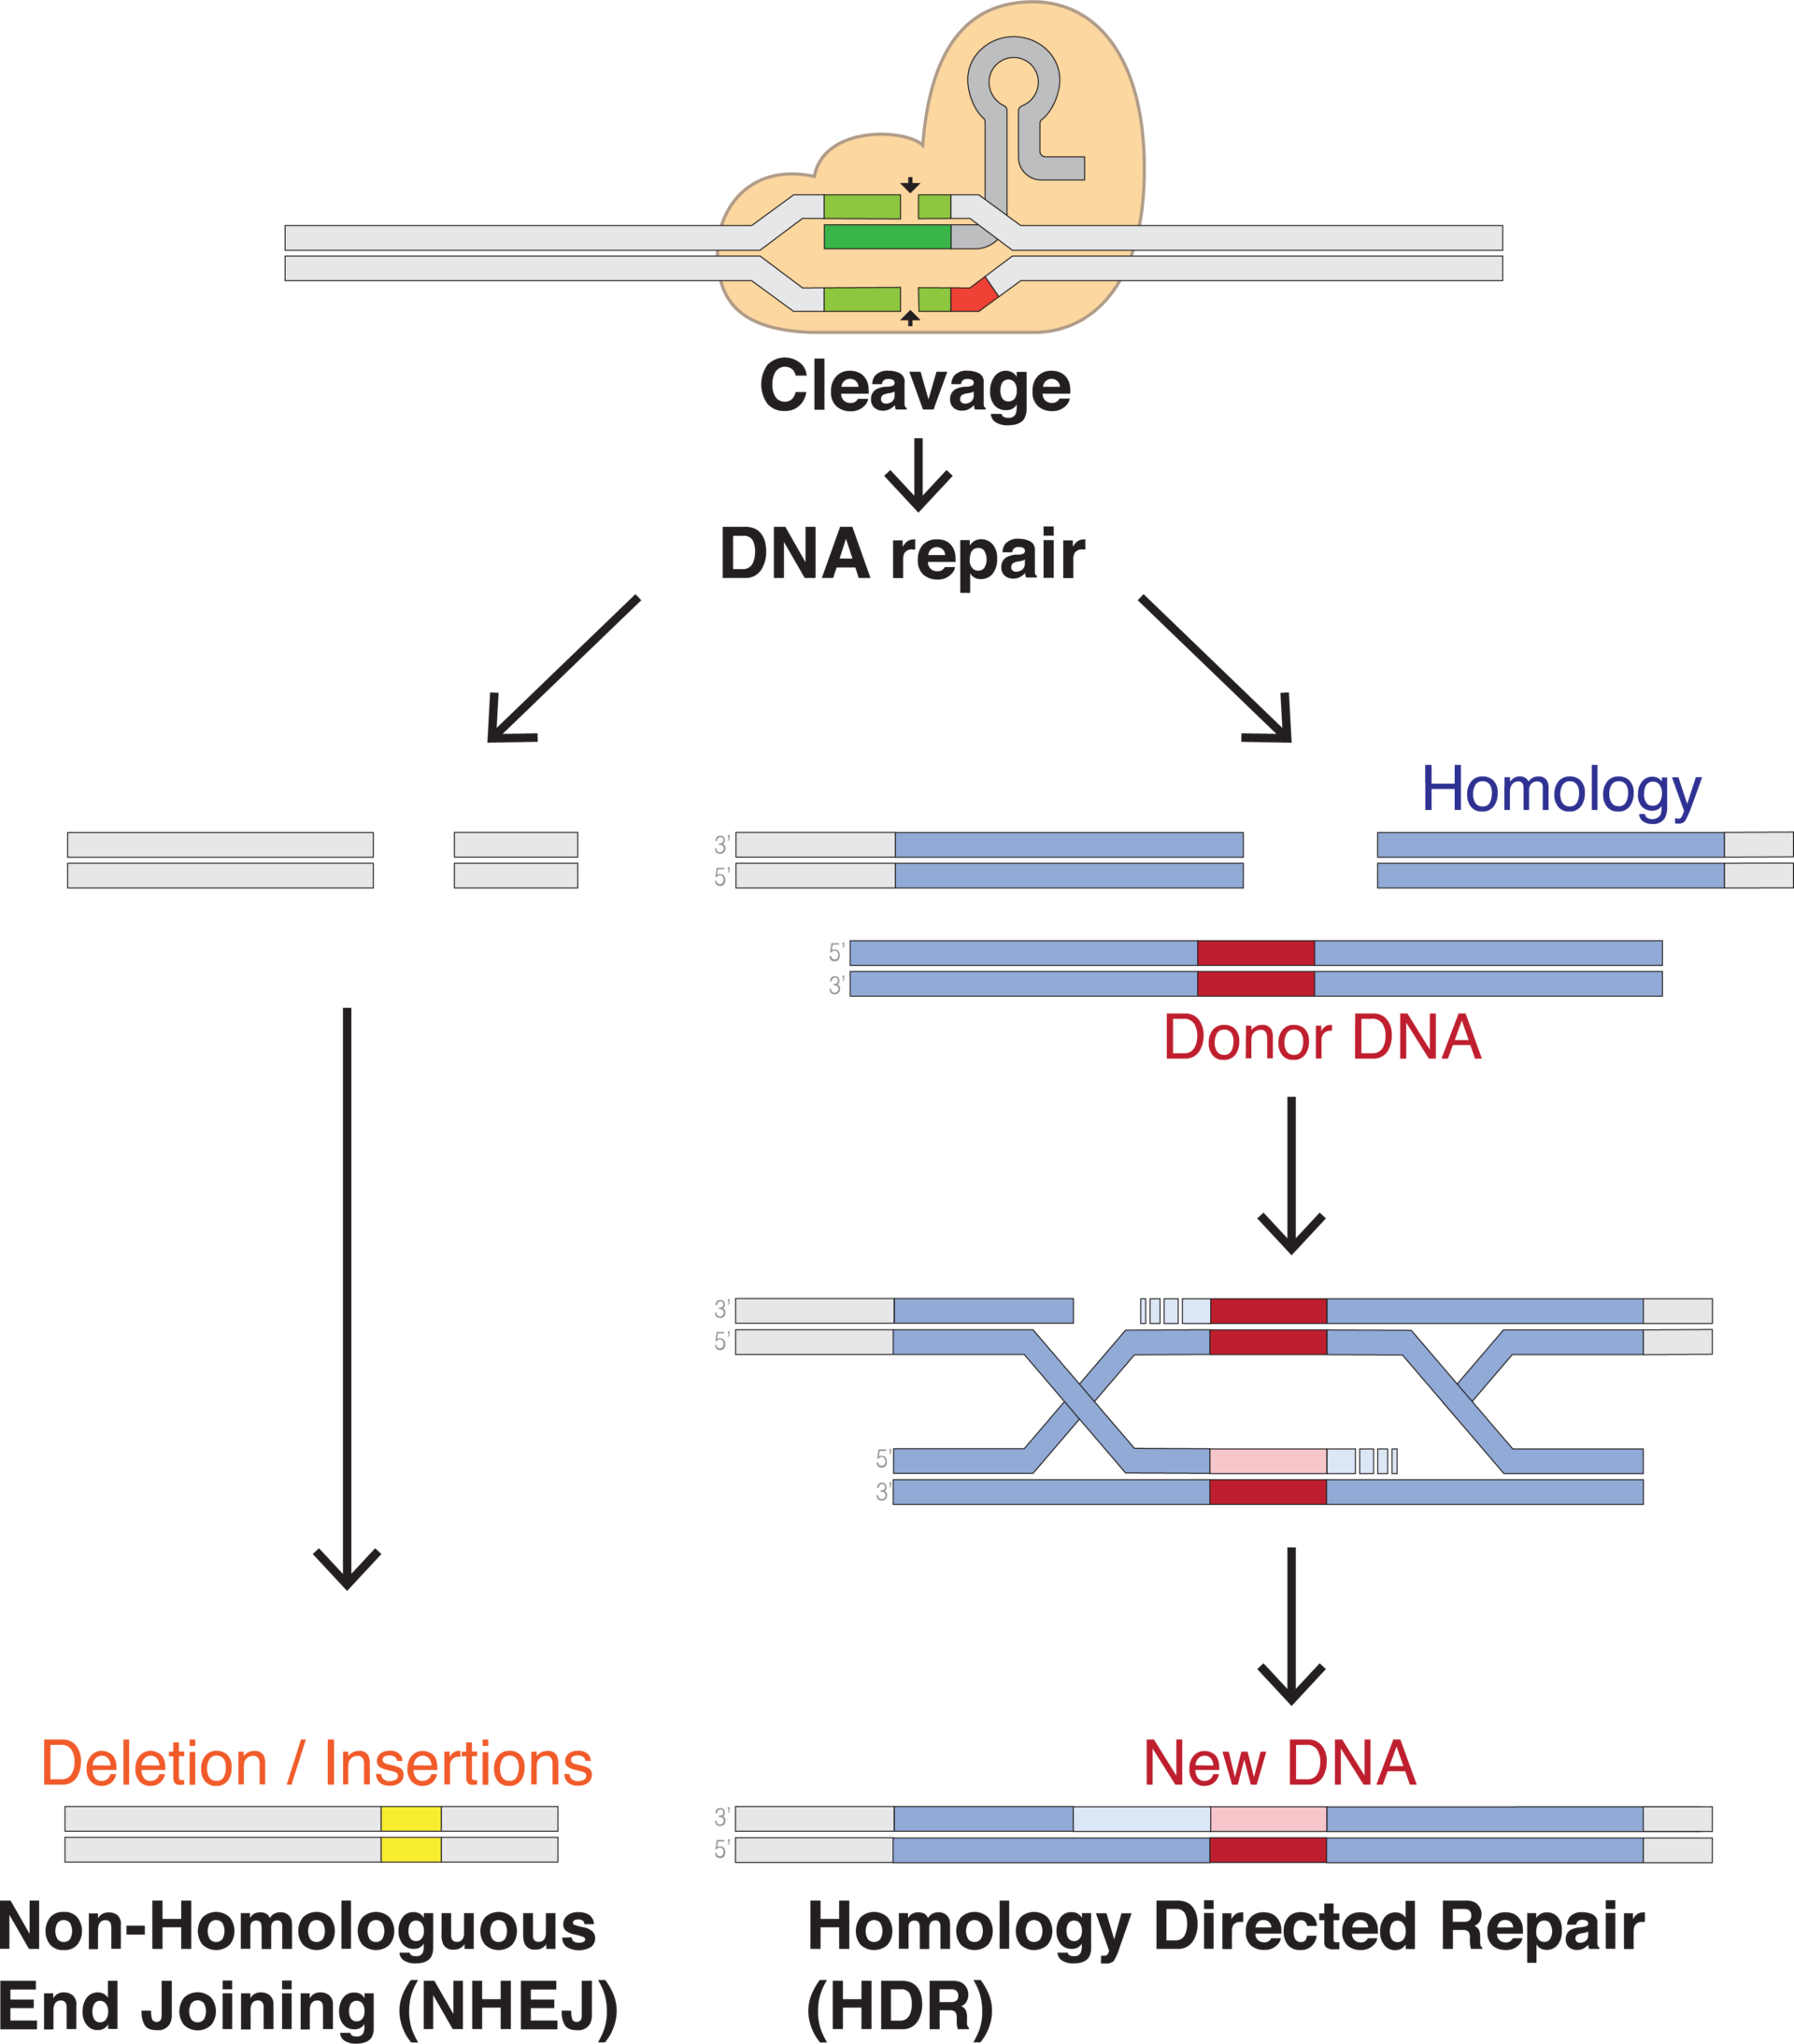
\includegraphics[width=\textwidth]{figures/crispr.png}
	\caption[CRISPR gene editing via HDR and NHEJ]{\textbf{CRISPR gene editing via HDR and NHEJ.}}
	\label{fig:crispr}
\end{figure} 
Since CRISPR-Cas9 enables a targeted random gene disruption, designing gRNA finely guiding Cas9 to the desired target sequence (\emph{on-targets}) is fundamental to avoid unexpected and dangerous outcomes on undesired targeted sequences (\emph{off-targets}). 
Most importantly, genetic variants may alter protospacer and PAM sequences and may influence both on-target and off-target potential. Therefore, it is fundamental to consider genetic variability when designing gRNA, to avoid potential undesired and dangerous outcomes on the host genome, in particular in clinical settings.
% ------ CRISPRme
\mychapter{7}{CRISPRme}
CRISPR-based systems may create unintended off-target modifications posing potential genotoxicity for therapeutic use. Several experimental assays and computational methods are available to uncover or forecast these off-targets \citep{clement2020technologies}. Off-target sites are partially predictable based on homology to the spacer and PAM sequence. Beyond the number of mismatches or bulges, a variety of sequence features, like position of mismatch or bulge with respect to PAM or specific base changes, contribute to off-target potential \citep{clement2020technologies,bao2021tools,hsu2013dna,doench2016optimized}. Computational models can complement experimental approaches to off-target nomination in several respects: to triage gRNAs prior to experiments by predicting the number and cleavage potential of off-target sites and to prioritize target sites for experimental scrutiny.  Gene editing strategies designed to specifically recognize patient mutations may increase the likelihood of editing mutant alleles, whereas variants that reduce homology to the anticipated target may decrease the efficiency of the desired genetic modification. Although a variety of in vitro and cell-based experimental methods can be used to empirically nominate off-target sites, these methods either use homology to the reference genome as a criterion to define the search space and/or use a limited set of human donor genomes to evaluate off-target potential \citep{bao2021tools,chaudhari2020evaluation}. Therefore, computational methods may be especially useful to predict the impact of off-target sequences not found in reference genomes. Prior studies considering gRNAs targeting therapeutically relevant genes using population-based variant databases like the 1000 Genomes Project (1000G) \citep{siva20081000} and the Exome Aggregation Consortium \citep{karczewski2017exac} have highlighted how genetic variants can significantly alter the off-target landscape by creating novel and personal off-target sites not present in a single reference genome \citep{lessard2017human,scott2017implications}. Although these prior studies provide code to reproduce analyses, implementation choices make these tools not suitable to analyze large variant datasets and to consider higher numbers of mismatches. In addition, these methods ignore bulges between RNA:DNA hybrids, cannot efficiently model alternative haplotypes and indels, and require extensive computational skills to utilize. Several user-friendly websites have been developed to aid the design of gRNAs and to assess their potential off-targets \citep{concordet2018crispor,listgarten2018prediction,labun2019chopchop,park2015cas}. Even though variant-aware prediction is an important problem for genome editing interventions, these scalable graphical user interface (GUI) based tools do not account for genetic variants. In addition, these tools artificially limit the number of mismatches for the search and/or do not support DNA/RNA bulges. Therefore, designing gRNAs for therapeutic intervention using current widely available tools could miss important off-target sites that may lead to unwanted genotoxicity. A complete and exhaustive off-target search with an arbitrary number of mismatches, bulges, and genetic variants that is haplotype-aware is a computationally challenging problem that requires specialized and efficient data structures. We have recently developed a command line tool that partially solves these challenges called CRISPRitz \citep{cancellieri2020crispritz}. This tool uses optimized data structures to efficiently account for single variants, mismatches and bulges but with significant limitations \citep{cancellieri2020crispritz}. We substantially extended CRISPRitz by developing CRISPRme \citep{cancellieri2022human}, a tool to aid gRNA design with added support for haplotype-aware off-target enumeration, short indel variants and a flexible number of mismatches and bulges. CRISPRme is a unified, user-friendly web-based application that provides several reports to prioritize putative off-targets based on their risk in a population or individuals. CRISPRme is flexible to accept user-defined genomic annotations, which could include empirically identified off-target sites or cell type specific chromatin features. It can integrate population genetic variants from sets of phased individual variants (like those from 1000G), unphased individual variants (like those from the Human Genome Diversity Project, HGDP \citep{bergstrom2020insights}) and population-level variants (like those from the Genome Aggregation Database, gnomAD \citep{karczewski2020mutational}). Furthermore, it can accept personal genomes from individual subjects to identify and prioritize private off-targets due to variants specific to a single individual. Here we demonstrate the utility of CRISPRme by analyzing the off-target potential of a gRNA currently being tested in clinical trials for SCD and $\beta$-thalassemia \citep{frangoul2021crispr,canver2015bcl11a,wu2019highly}. We identify possible off-targets introduced by genetic variants included within and extending beyond 1000G. We predict that the most likely off-target site, overlooked by prior analyses, is introduced by a variant common in African-ancestry individuals (rs114518452, minor allele frequency (MAF)$=4.5\%$) and provide experimental evidence of its off-target potential in gene edited human CD34+ hematopoietic stem and progenitor cells. Furthermore, we demonstrate that alternative allele-specific off-target potential is widespread across various gRNAs and editors.
% ---- CRISPRme: a variant-aware computational tool to nominate candidate off-target sites
\section{CRISPRme: a variant-aware computational tool to nominate candidate off-target sites}
CRISPRme is a web-based tool to predict off-target potential of CRISPR gene editing that accounts for genetic variation. CRISPRme can also be deployed locally as a web app or used as a command line utility, both of which respect genomic privacy offline. CRISPRme takes as input a Cas protein, gRNA spacer sequence(s) and PAM, genome build, sets of variants (VCF files for populations or individuals), user-defined thresholds of mismatches and bulges, and optional user-defined genomic annotations to produce comprehensive and personalized reports (\textbf{Fig.\ref{fig:crisprme1} (A)}).
\begin{figure}
	\centering
	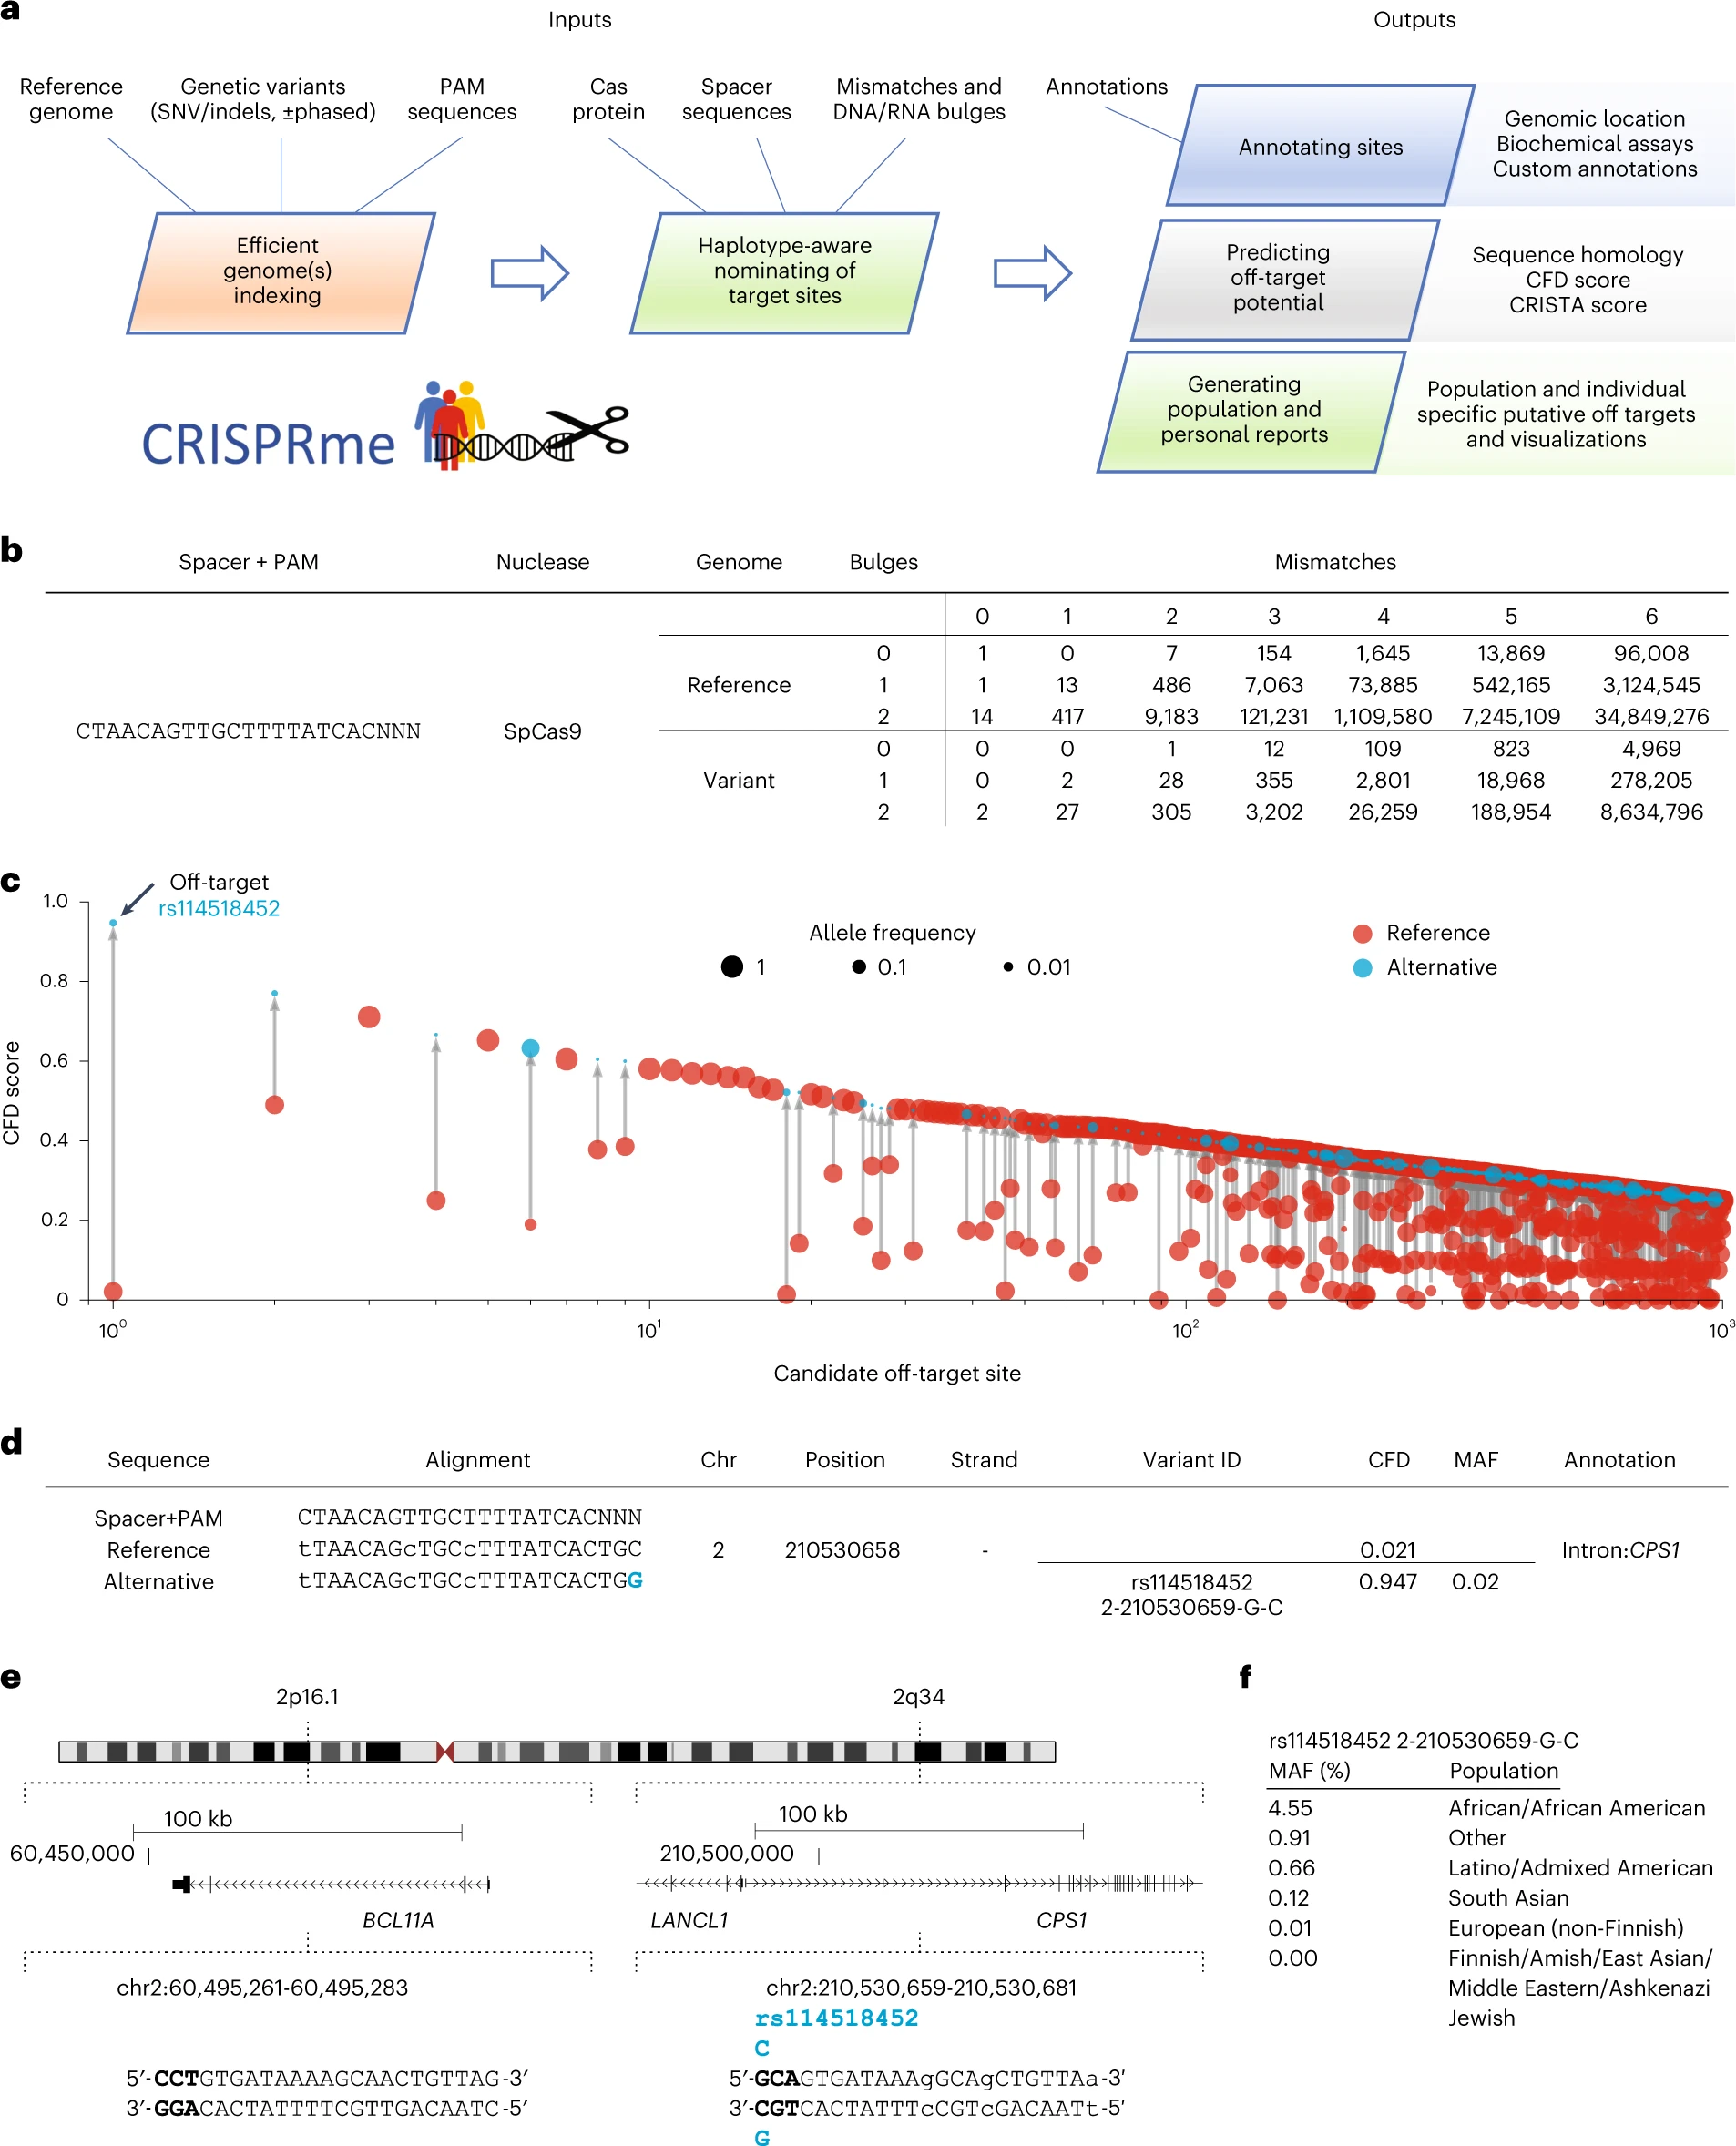
\includegraphics[width=\textwidth]{figures/crisprme1.png}
	\caption[CRISPRme provides web-based analysis of CRISPR-Cas gene editing off-target potential reflecting population genetic diversity]{\textbf{CRISPRme provides web-based analysis of CRISPR-Cas gene editing off-target potential reflecting population genetic diversity. (A)} CRISPRme software takes as input a reference genome, genetic variants, PAM sequence, Cas protein type, spacer sequence, homology threshold and genomic annotations and provides comprehensive, target-focused and individual-focused analyses of off-target potential. It is available as an online webtool and can be deployed locally or used offline as command-line software. \textbf{(B)} Analysis of the BCL11A-1617 spacer targeting the +58 erythroid enhancer with SpCas9, \texttt{NNN} PAM, 1000G variants, up to 6 mismatches and up to 2 bulges. \textbf{(C)} Top 1000 predicted off-target sites ranked by CFD score, indicating the CFD score of the reference and alternative allele if applicable, with allele frequency indicated by circle size. \textbf{(D)} The off-target site with the highest CFD score is created by the minor allele of rs114518452. Coordinates are for hg38 and 0-start for the potential off-target and 1-start for the variant-ID. MAF is based on 1000G. \textbf{(E)} The top predicted off-target site from CRISPRme is an allele-specific off-target with 3 mismatches to the BCL11A-1617 spacer sequence, where the rs114518452-C minor allele produces a de novo NGG PAM sequence. PAM sequence shown in bold and mismatches to BCL11A-1617 shown as lowercase. Coordinates are for hg38 and 1-start. \textbf{(F)} rs114518452 allele frequencies based on gnomAD v3.1. Coordinates are for hg38 and 1-start. Spacer shown as DNA sequence for ease of visual alignment.}
	\label{fig:crisprme1}
\end{figure} 
We designed CRISPRme to be flexible with support for new gene editors with variable and extremely relaxed PAM requirements \citep{walton2020unconstrained}. Thanks to a PAM encoding based on Aho-Corasick automata and an index based on a ternary search tree, CRISPRme can perform genome-wide exhaustive searches efficiently even with an \texttt{NNN} PAM, extensive mismatches (tested with up to 7) and RNA:DNA bulges (tested with up to 2). Notably, a comprehensive search performed with up to 6 mismatches, 2 DNA/RNA bulges and a fully non-restrictive PAM (\texttt{NNN}) takes only 24 hours on a small computational cluster node (Intel Xeon CPU E5-2609 v4 clocked at 2.2 GHz and 128 GB RAM). All the 1000G variants, including both SNVs and indels, can be included in the search together with all the available metadata for each individual (sex, super-population and age), and the search operation takes into account observed haplotypes. Importantly, off-target sites that represent alternative alignments to a given genomic region are merged to avoid inflating the number of reported sites. Although several tools exist to enumerate off-targets, to our knowledge only two command line tools \citep{lessard2017human,fennell2021calitas} incorporate genetic variants in the search. However, they have several limitations in terms of scalability to large searches, number of mismatches, bulges, haplotypes, and variant file formats supported and do not provide an easy-to-use graphical user interface. CRISPRme generates several reports. (i) It summarizes for each gRNA all the potential off-targets found in the reference or variant genomes based on their mismatches and bulges (\textbf{Fig.\ref{fig:crisprme1} (B)}) and generates a file with detailed information on each of these candidate off-targets. (ii) It compares gRNAs to customizable annotations. By default, it classifies possible off-target sites based on GENCODE22 (genomic features) and ENCODE23 (candidate cis-regulatory elements, cCREs) annotations. It can also incorporate user-defined annotations in BED format, such as empiric off-target scores or cell type specific chromatin features (\textbf{Fig.\ref{fig:crisprme2}}). 
\begin{figure}
	\centering
	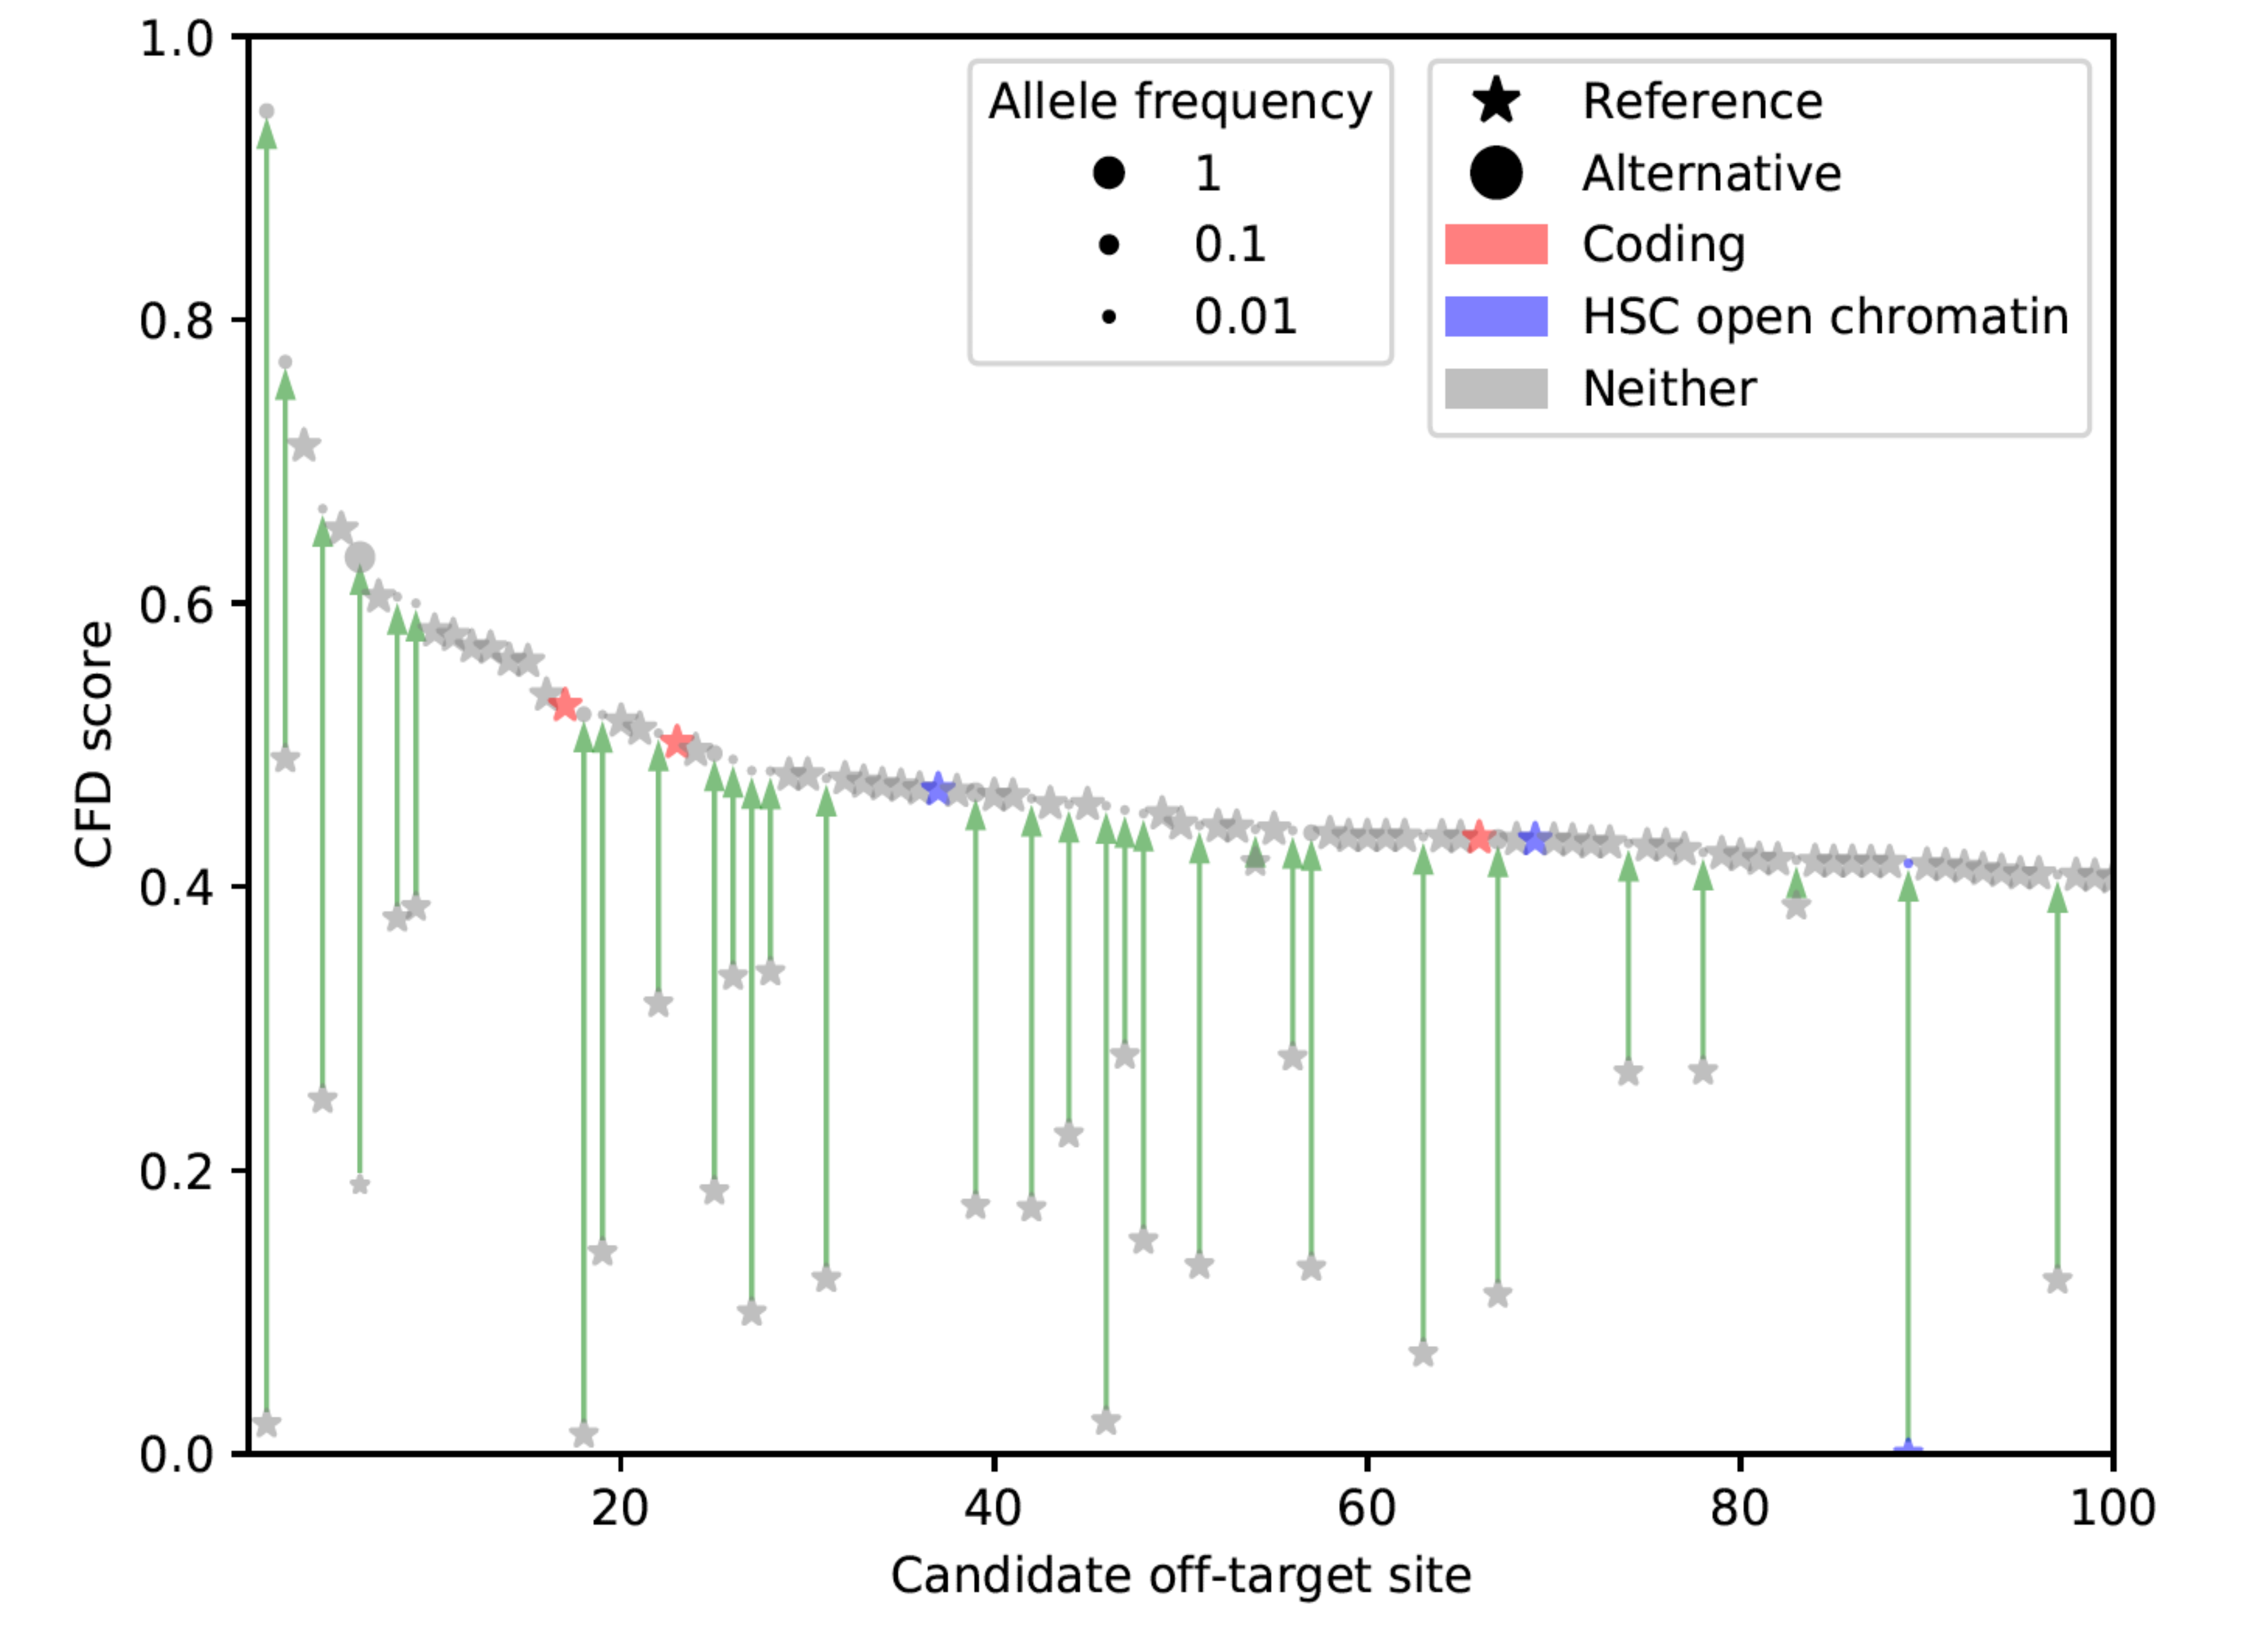
\includegraphics[width=\textwidth]{figures/crisprme2.png}
	\caption[Top 100 predicted off-target sites for BCL11A-1617 spacer by CFD score]{\textbf{Top 100 predicted off-target sites for BCL11A-1617 spacer by CFD score.} CRISPRme search as in \textbf{Fig.\ref{fig:crisprme1}}. Candidate off-target sites within coding regions based on GENCODE annotations and ATAC-seq peaks in HSCs based on user-provided annotations are highlighted.}
	\label{fig:crisprme2}
\end{figure} 
(iii) Using 1000G and/or HGDP16 variants, CRISPRme reports the cumulative distribution of homologous sites based on the reference genome or super-population. These global reports could be used to compare a set of gRNAs based on how genetic variation impacts their predicted on- and off-target cleavage potential using cutting frequency determination (CFD) or CRISPR Target Assessment (CRISTA) \citep{abadi2017machine} scores (\textbf{Fig.\ref{fig:crisprme3}}). 
\begin{figure}
	\centering
	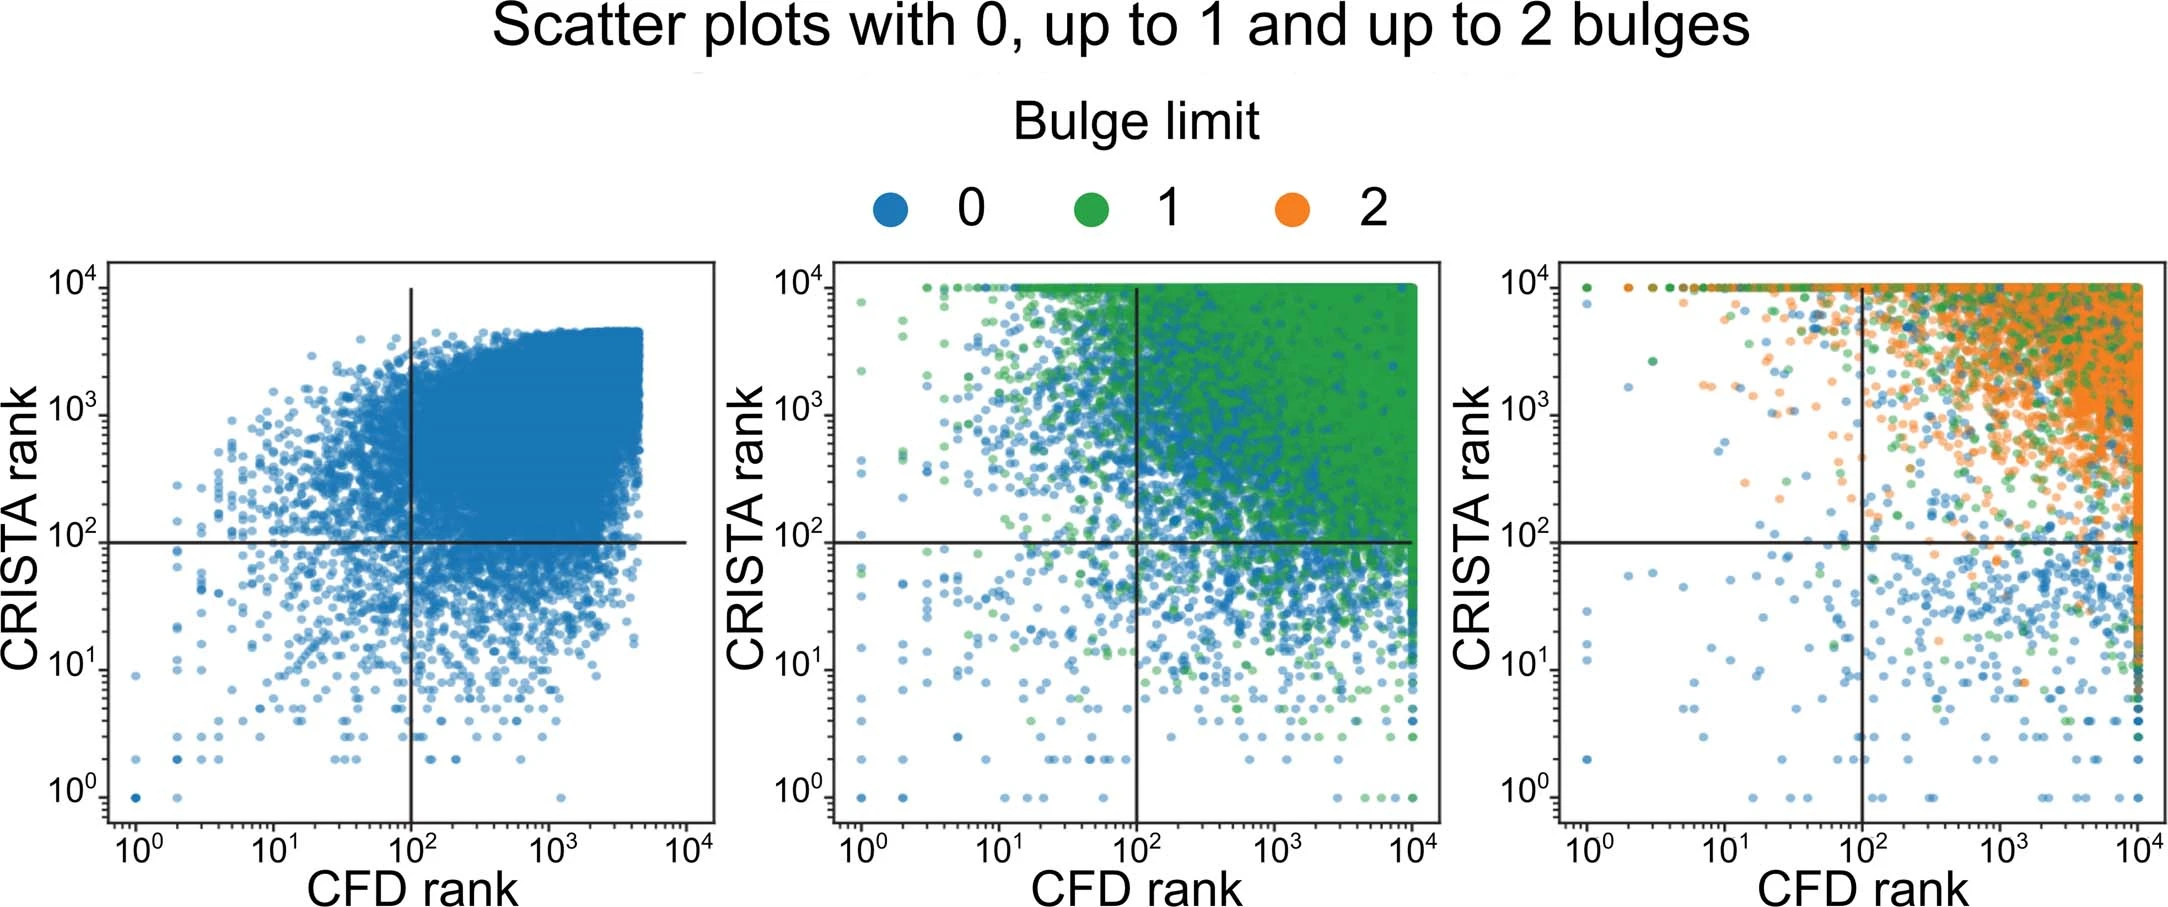
\includegraphics[width=\textwidth]{figures/crisprme3.png}
	\caption[Plots with rank ordered correlation between CFD and CRISTA reported targets]{\textbf{Plots with rank ordered correlation between CFD and CRISTA reported targets.} Scatter plots show from left to right, the correlation of ranked targets, extracted by selecting top $10000$ targets ordered by CFD and CRISTA score, respectively. The left plot shows the rank correlation of targets with $0$ bulges (Pearson’s correlation: $0.57$, $p < 1e^{-10}$, Spearman’s correlation: $0.55, p < 1e^{-10}$), the center plot shows rank correlation of targets with $1$ bulge (Pearson’s correlation: $-0.16, p < 1 e^{-10}$, Spearman’s correlation: $-0.33, p < 1e^{-10}$) and the right plot shows the rank correlation of targets with $2$ bulges (Pearson’s correlation: $-0.55, p < 1e^{-10}$, Spearman’s correlation: $-0.80, p < 1e^{-10}$). The correlation values and $P$-values(two-sided) were calculated using standard functions from the Python scipy library.The colors represent the lowest count of bulges for each target, since the two scoring methods may prioritize different alignments and thus different number of mismatches and bulges of the same genomic target.}
	\label{fig:crisprme3}
\end{figure} 
CRISPRme includes multiple scoring metrics and can be easily extended with new ones, including scores tailored for different editors. Finally, CRISPRme can generate personal genome focused reports called personal risk cards. These reports highlight private off-target sites due to unique genetic variants.
% ---- Results
\section{Results}
We tested CRISPRme with a gRNA (\#1617) targeting a GATA1 binding motif at the +58 erythroid enhancer of BCL11A18,19. A recent clinical report described two patients, one with SCD and one with $\beta$-thalassemia, each treated with autologous gene modified hematopoietic stem and progenitor cells (HSPCs) edited with Cas9 and this gRNA, who showed sustained increases in fetal hemoglobin, transfusion-independence and absence of vaso-occlusive episodes (in the SCD patient) following therapy. This study as well as prior pre-clinical studies with the same gRNA (\#1617) did not reveal evidence of off-target editing in treated cells when considering off-target sites nominated by bioinformatic analysis of the human reference genome and empiric analysis of in vitro genomic cleavage potential \citep{frangoul2021crispr,wu2019highly,demirci2019durable}. CRISPRme analysis found that the predicted off-target site with both the greatest CFD score and the greatest increase in CFD score from the reference to alternative allele was at an intronic sequence of CPS1 (\textbf{Fig.\ref{fig:crisprme1} (C)} and \textbf{(D)}), a genomic target subject to common genetic variation (modified by a SNP with MAF $\geq 1\%$). CFD scores range from 0 to 1, where the on-target site has a score of 1. The alternative allele rs114518452-\texttt{C} generates a \texttt{TGG} PAM sequence (that is, the optimal PAM for SpCas9) for a potential off-target site with 3 mismatches and a CFD score (CFDalt 0.95) approaching that of the on-target site (\textbf{Fig.\ref{fig:crisprme1} (E)}). In contrast, the reference allele rs114518452-\texttt{G} disrupts the PAM to \texttt{TGC}, which markedly reduces predicted cleavage potential (CFDref 0.02). rs114518452-\texttt{C} has an overall MAF of $1.33\%$ in gnomAD v3.1, with MAF of $4.55\%$ in African/African-American, $0.9\%$ in Other, $0.07\%$ in Latino/Admixed American, $0.02\%$ in European (non-Finnish) and $0.00\%$ in East Asian populations (\textbf{Fig.\ref{fig:crisprme1} (F)}). To consider the off-target potential that could be introduced by personal genetic variation that would not be predicted by 1000G variants, we analyzed HGDP variants identified from whole genome sequences of 929 individuals from 54 diverse human populations. We observed 249 candidate off-targets for gRNA \#1617 with CFD $\geq 0.2$ for which the CFD score in HGDP exceeded that found for either the reference genome or 1000G variants by at least $0.1$ (\textbf{Fig.\ref{fig:crisprme4} (A)} and \textbf{Fig.\ref{fig:crisprme5}}). 
\begin{figure}
	\centering
	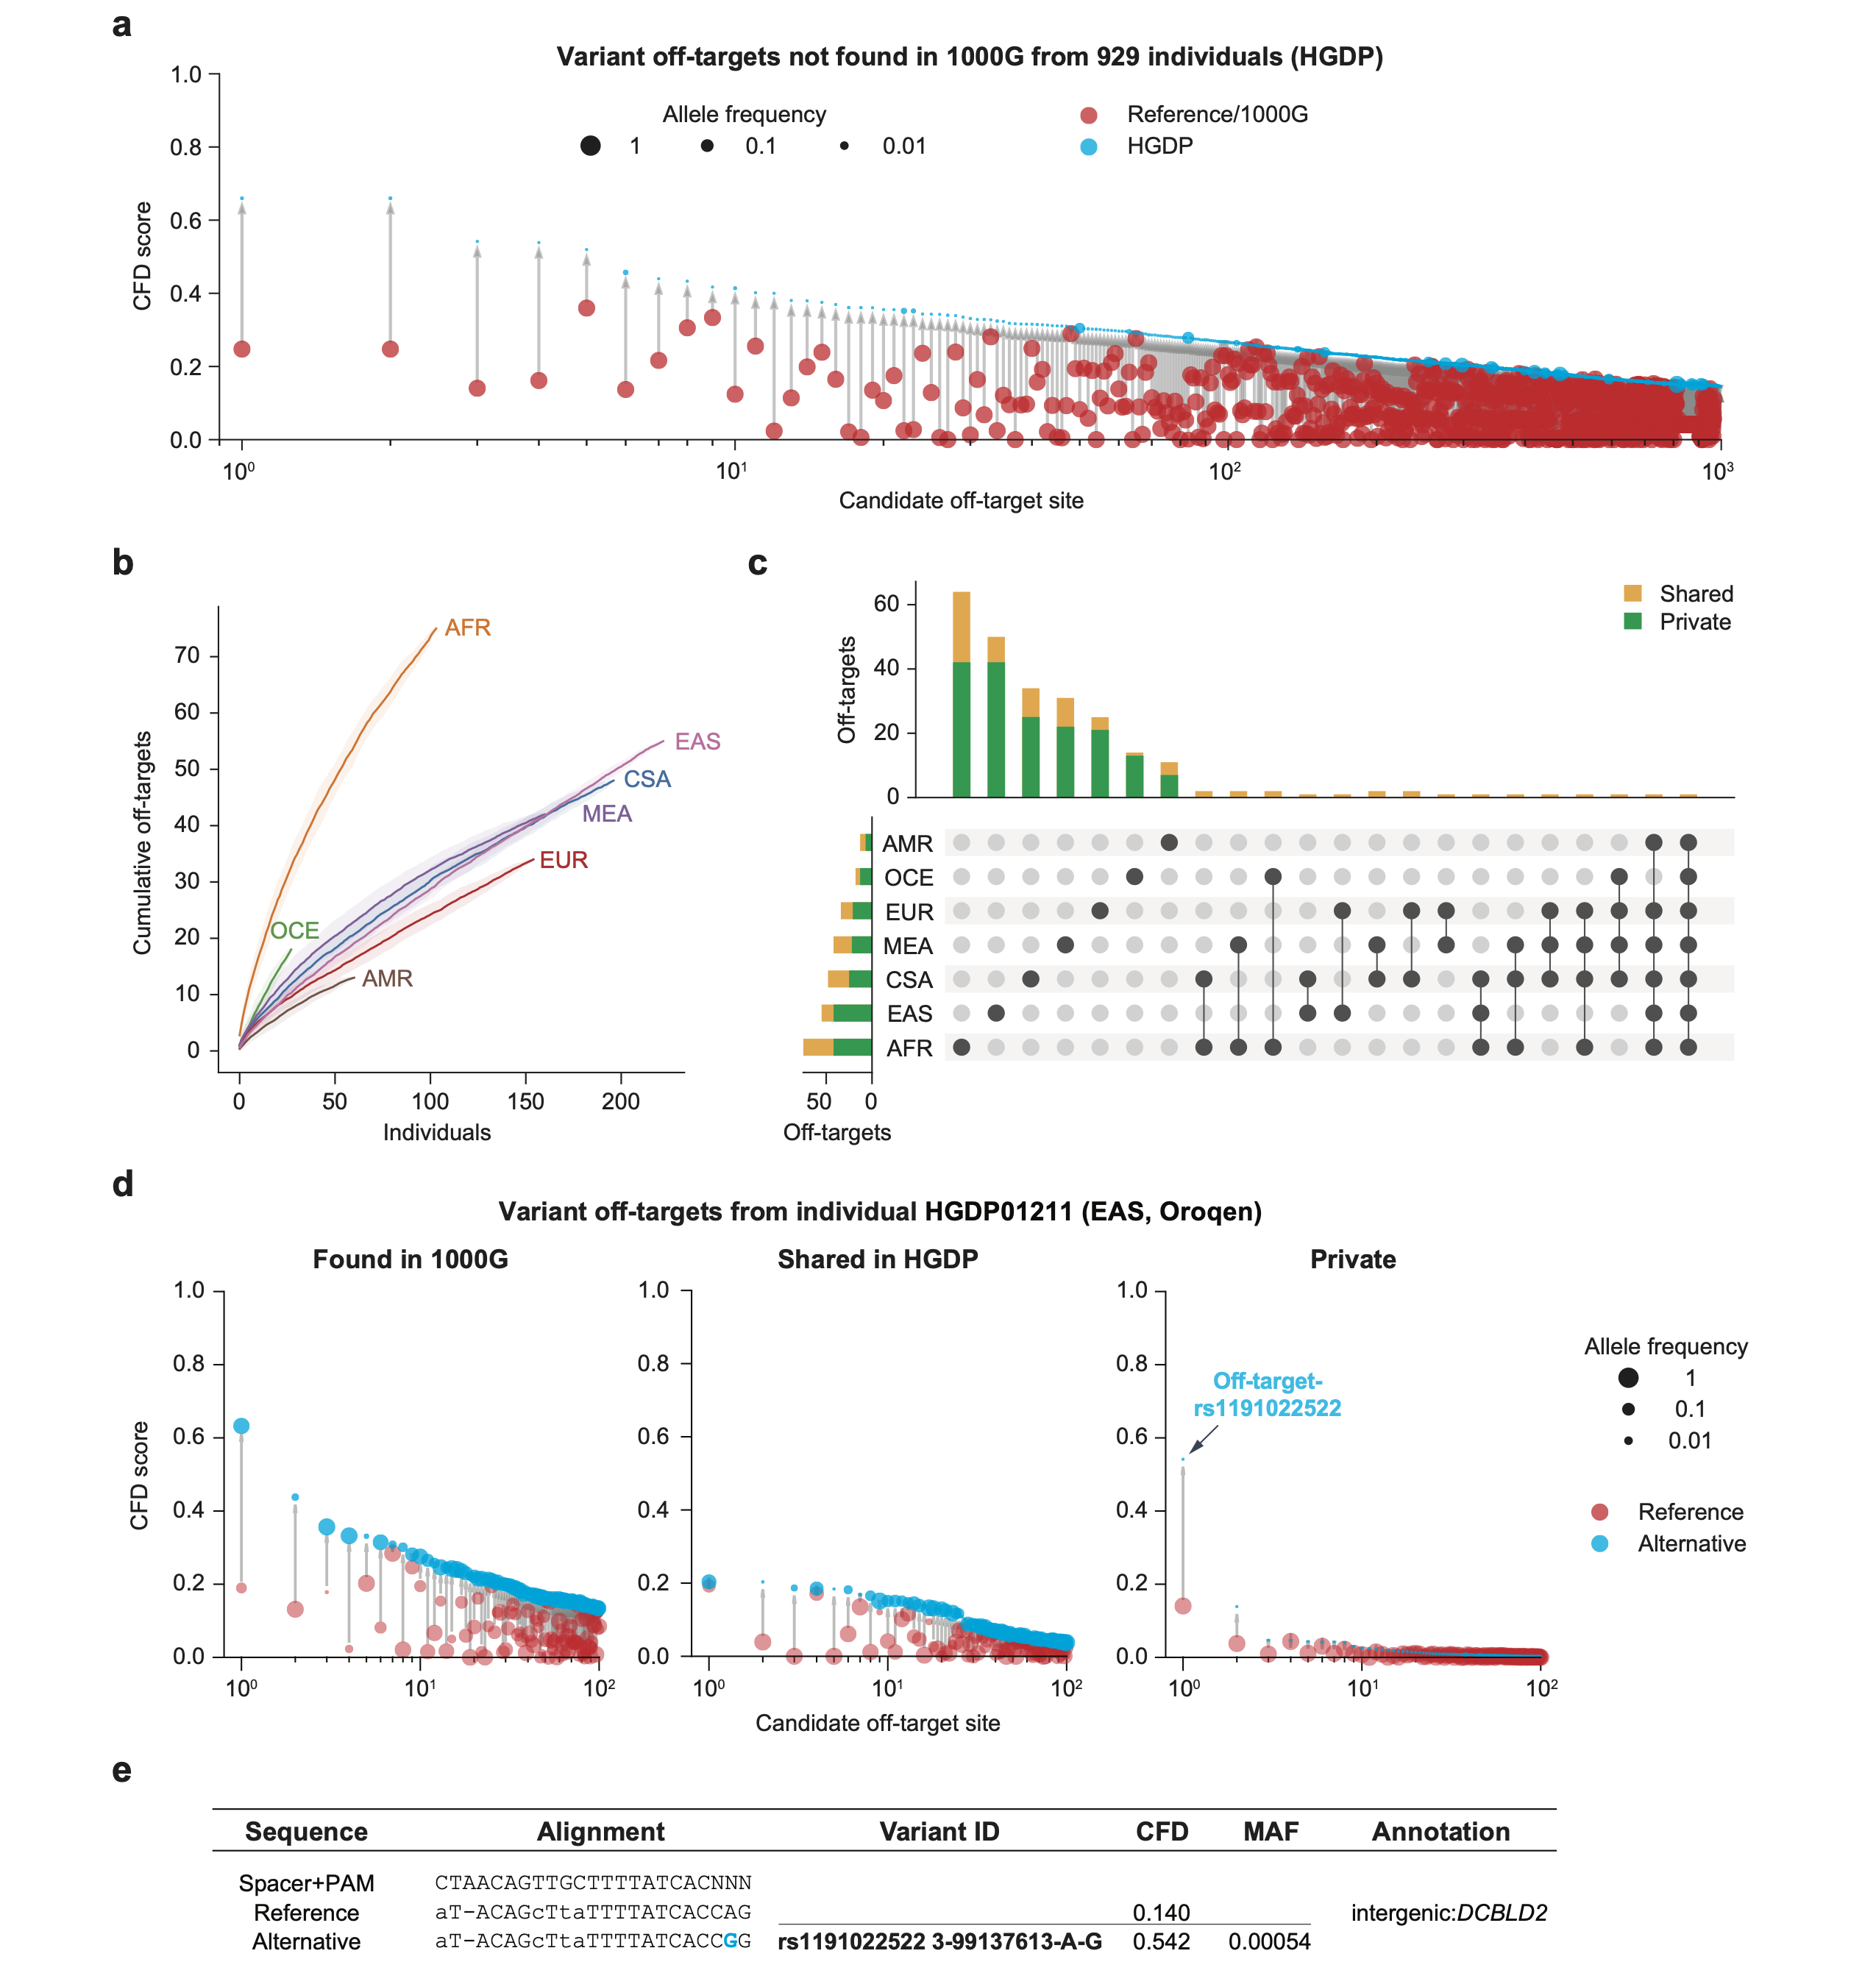
\includegraphics[width=\textwidth]{figures/crisprme4.png}
	\caption[CRISPRme provides analysis of off-target potential of CRISPR-Cas gene editing reflecting population and private genetic diversity]{\textbf{CRISPRme provides analysis of off-target potential of CRISPR-Cas gene editing reflecting population and private genetic diversity. (A)} CRISPRme analysis was conducted with variants from HGDP comprising whole genome sequencing of 929 individuals from 54 diverse human populations. HGDP variant off-targets with greater CFD scores than the reference genome or 1000G were plotted and sorted by CFD score, with HGDP variant off-targets shown in blue and reference or 1000G variant off-targets shown in red. \textbf{(B)} HGDP variant off-targets with CFD $\geq 0.2$ and increase in CFD of $\geq 0.1$. Individual samples from each of the seven super-populations were shuffled 100 times to calculate the mean and 95\% confidence interval. \textbf{(C)} Intersection analysis of HGDP variant off-targets with CFD $\geq 0.2$ and increase in CFD of $\geq 0.1$. Shared variants were found in 2 or more HGDP samples while private variants were limited to a single sample. \textbf{(D)} CRISPRme analysis of a single individual (HGDP01211) showing the top 100 variant off-targets from each of the following three categories: shared with 1000G variant off-targets (left panel), higher CFD score compared to reference genome and 1000G but shared with other HGDP individuals (center panel), and higher CFD score compared to reference genome and 1000G with variant not found in other HGDP individuals (right panel). For the center and right panels, reference refers to CFD score from reference genome or 1000G variants. \textbf{(E)} The top predicted private off-target site from HGDP01211 is an allele-specific off-target where the rs1191022522-\texttt{G} minor allele produces a canonical \texttt{NGG} PAM sequence in place of a noncanonical \texttt{NAG} PAM sequence. Spacer shown as DNA sequence for ease of visual alignment.}
	\label{fig:crisprme4}
\end{figure} 
\begin{figure}
	\centering
	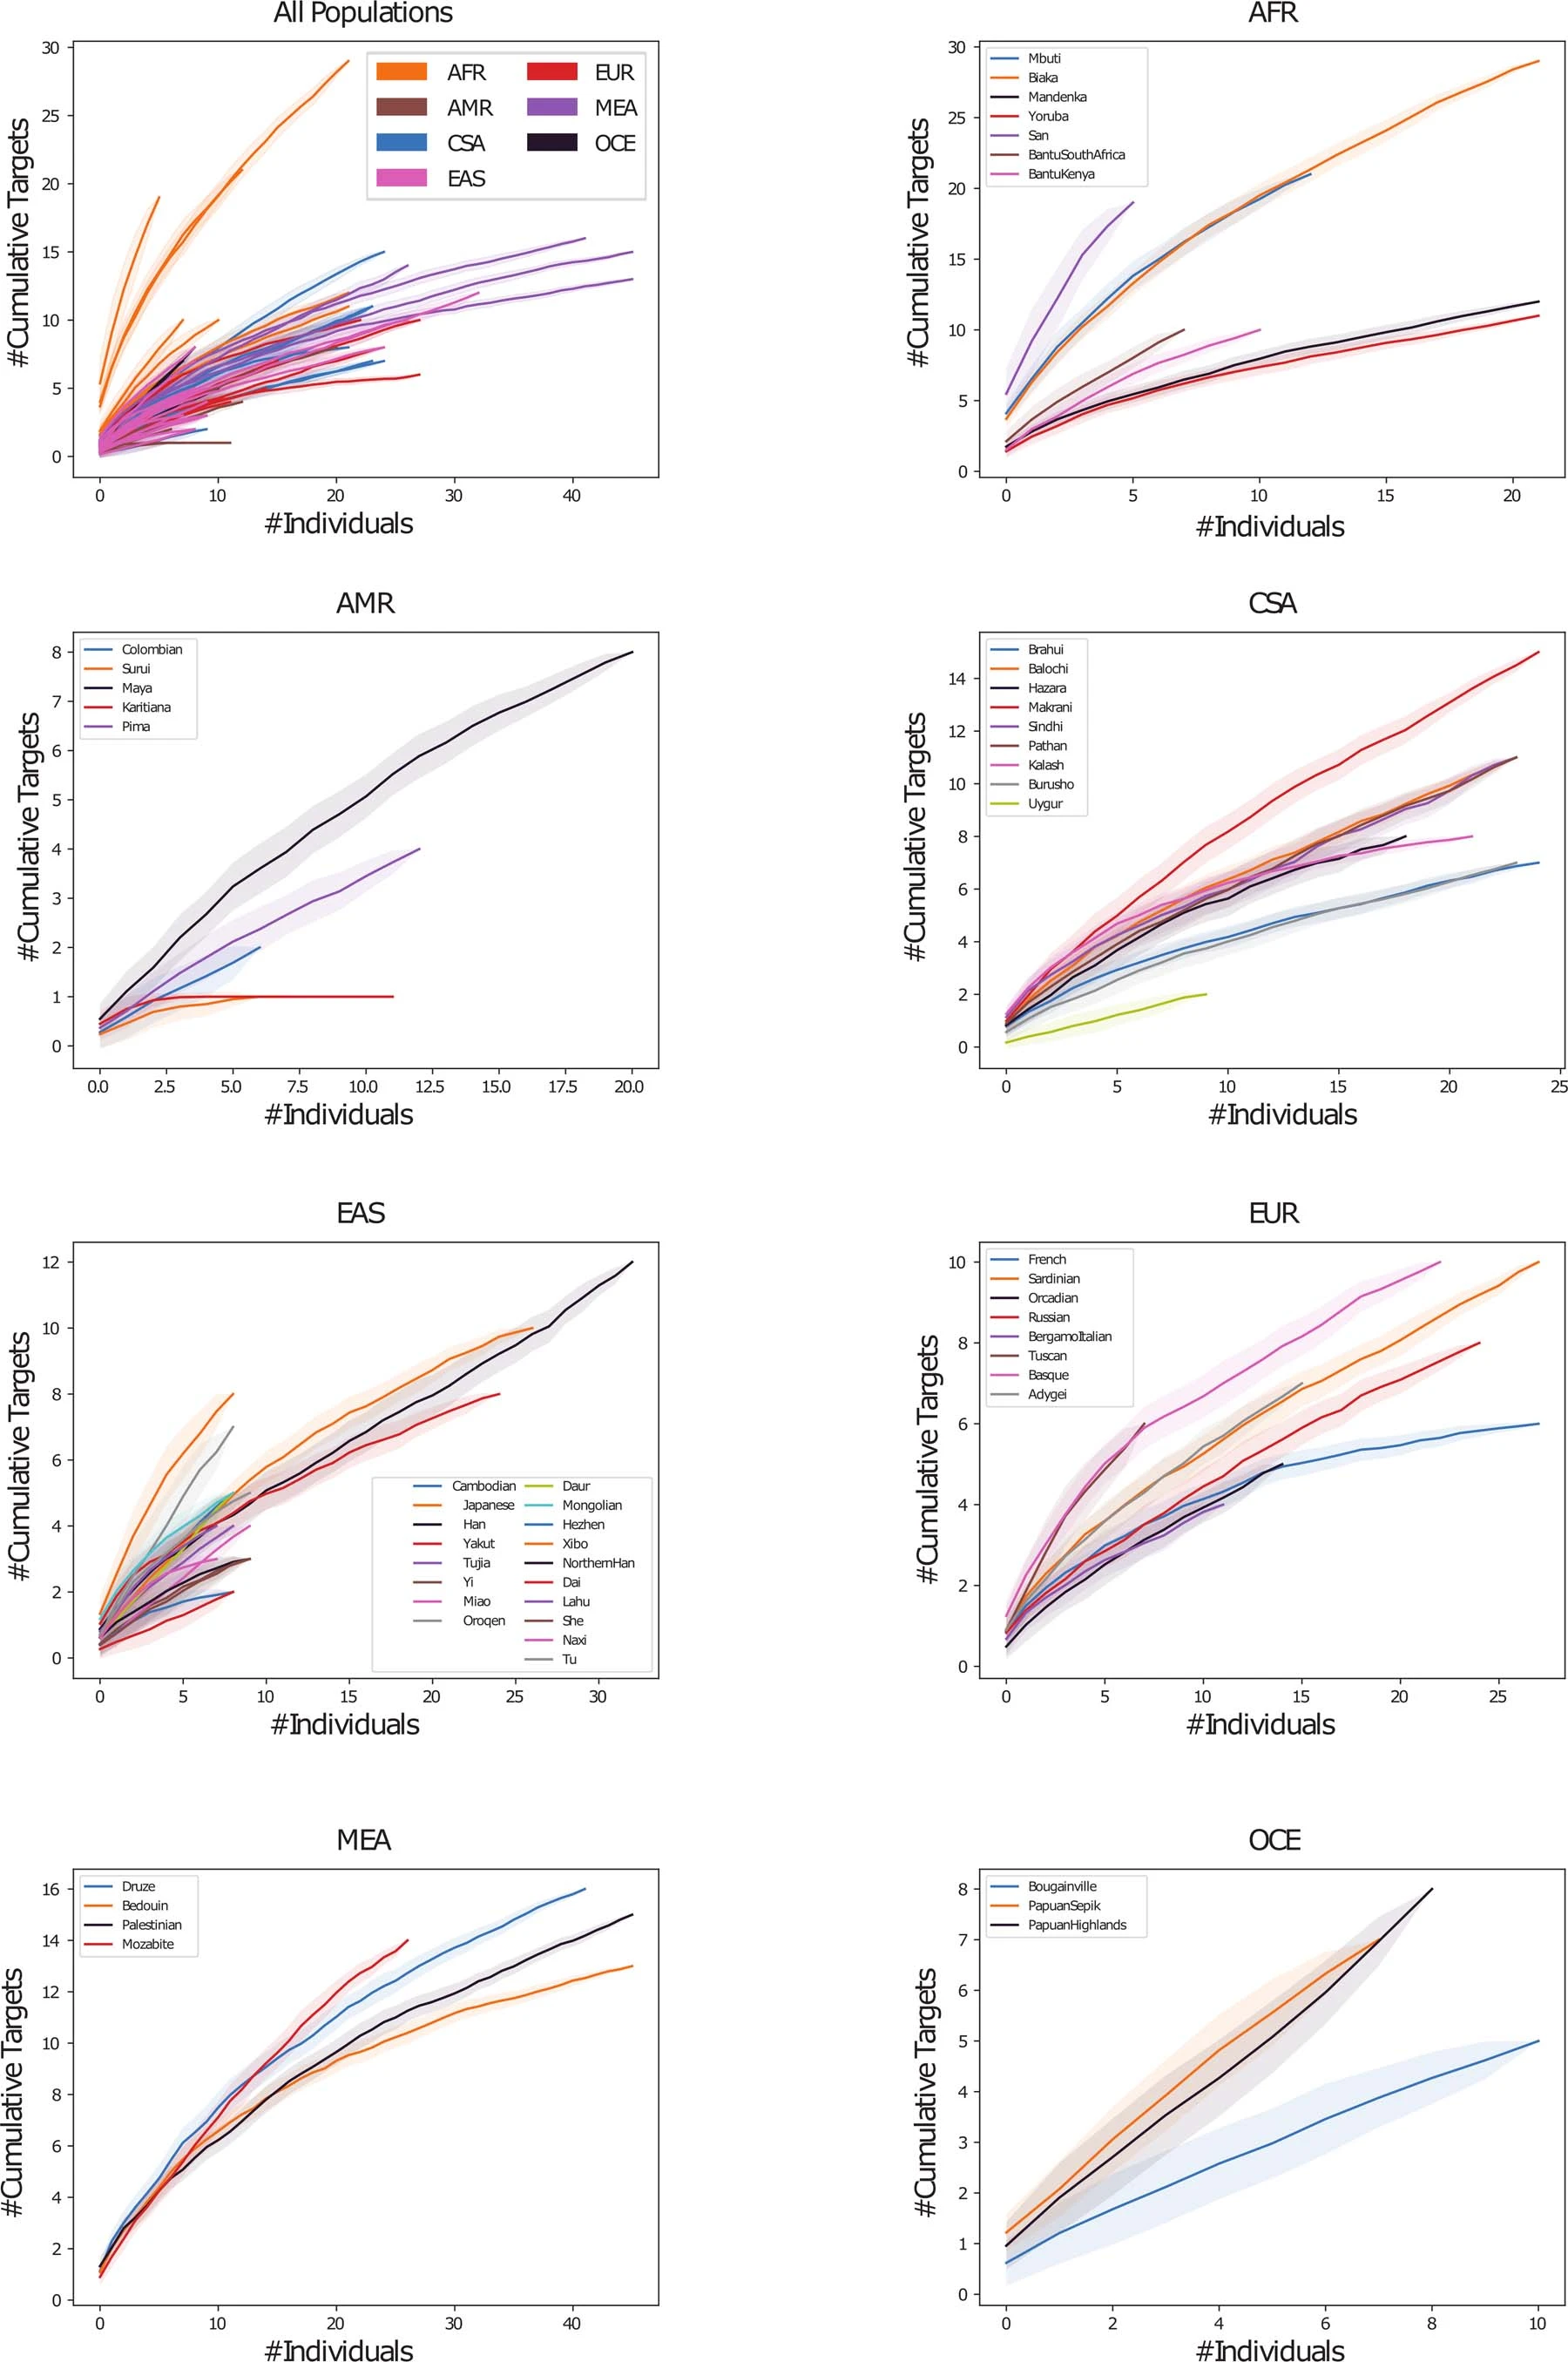
\includegraphics[width=\textwidth]{figures/crisprme5.png}
	\caption[HGDP super-population distribution plots]{\textbf{HGDP super-population distribution plots.} HGDP variant off-targets with CFD $\geq 0.2$ and increase in CFD of $\geq 0.1$. Individual samples from each of the seven super-populations were shuffled 100 times to calculate the mean and 95\% confidence interval. First panel shows distribution within all 54 discrete populations, colored by super-population. Additional seven panels show distribution of discrete populations within each listed super-population.}
	\label{fig:crisprme5}
\end{figure} 
These additional variant off-targets not found from 1000G were observed in each super-population, with the greatest frequency in the African super-population (\textbf{Fig.\ref{fig:crisprme4} (B)}). 229 (92.0\%) of these variant off-targets were unique to a super-population and 172 (69.1\%) of these were private to just one individual (\textbf{Fig.\ref{fig:crisprme4} (C)}). Furthermore, single individual focused searches, for example an analysis of HGDP01211, an individual of the Oroqen population within the East Asian super-population, showed that most variant off-targets (with higher CFD score than reference) were due to variants also found in 1000G (n=32369, 90.4\%), a subset were due to variants shared with other individuals from HGDP but absent from 1000G (n=3177, 8.9\%), and a small fraction were private to the individual (n=234, 0.7\%) (\textbf{Fig.\ref{fig:crisprme4} (D)}). Among these private off-targets was one generated by a variant (rs1191022522, 3-99137613-\texttt{A}-\texttt{G}, gnomAD v3.1 MAF 0.0053\%) where the alternative allele produces a canonical \texttt{NGG} PAM that increases the CFD score from $0.14$ to $0.54$ (\textbf{Fig.\ref{fig:crisprme4} (D)} and \textbf{(E)}). To experimentally test the top predicted off-target from CRISPRme, we identified a CD34+ HSPC donor of African ancestry heterozygous for rs114518452-\texttt{C}, the variant predicted to introduce the greatest increase in off-target cleavage potential (\textbf{Fig.\ref{fig:crisprme1} (C-F)}). We performed RNP electroporation using a gene editing protocol that preserves engrafting HSC function. Amplicon sequencing analysis showed $92.0 \pm 0.5\%$ indels at the on-target site and $4.8 \pm 0.5\%$ indels at the off-target site. For reads spanning the variant position, indels were strictly found at the alternative PAM-creation allele without indels observed at the reference allele (\textbf{Fig.\ref{fig:crisprme6} (A-C)}), suggesting $9.6 \pm 1.0\%$ off-target editing of the alternative allele. In an additional 6 HSPC donors homozygous for the reference allele rs114518452-\texttt{G}/\texttt{G}, $0.00 \pm 0.00\%$ indels were observed at the off-target site, suggesting strict restriction of off-target editing to the alternative allele (\textbf{Fig.\ref{fig:crisprme6} (D)}). 
\begin{figure}
	\centering
	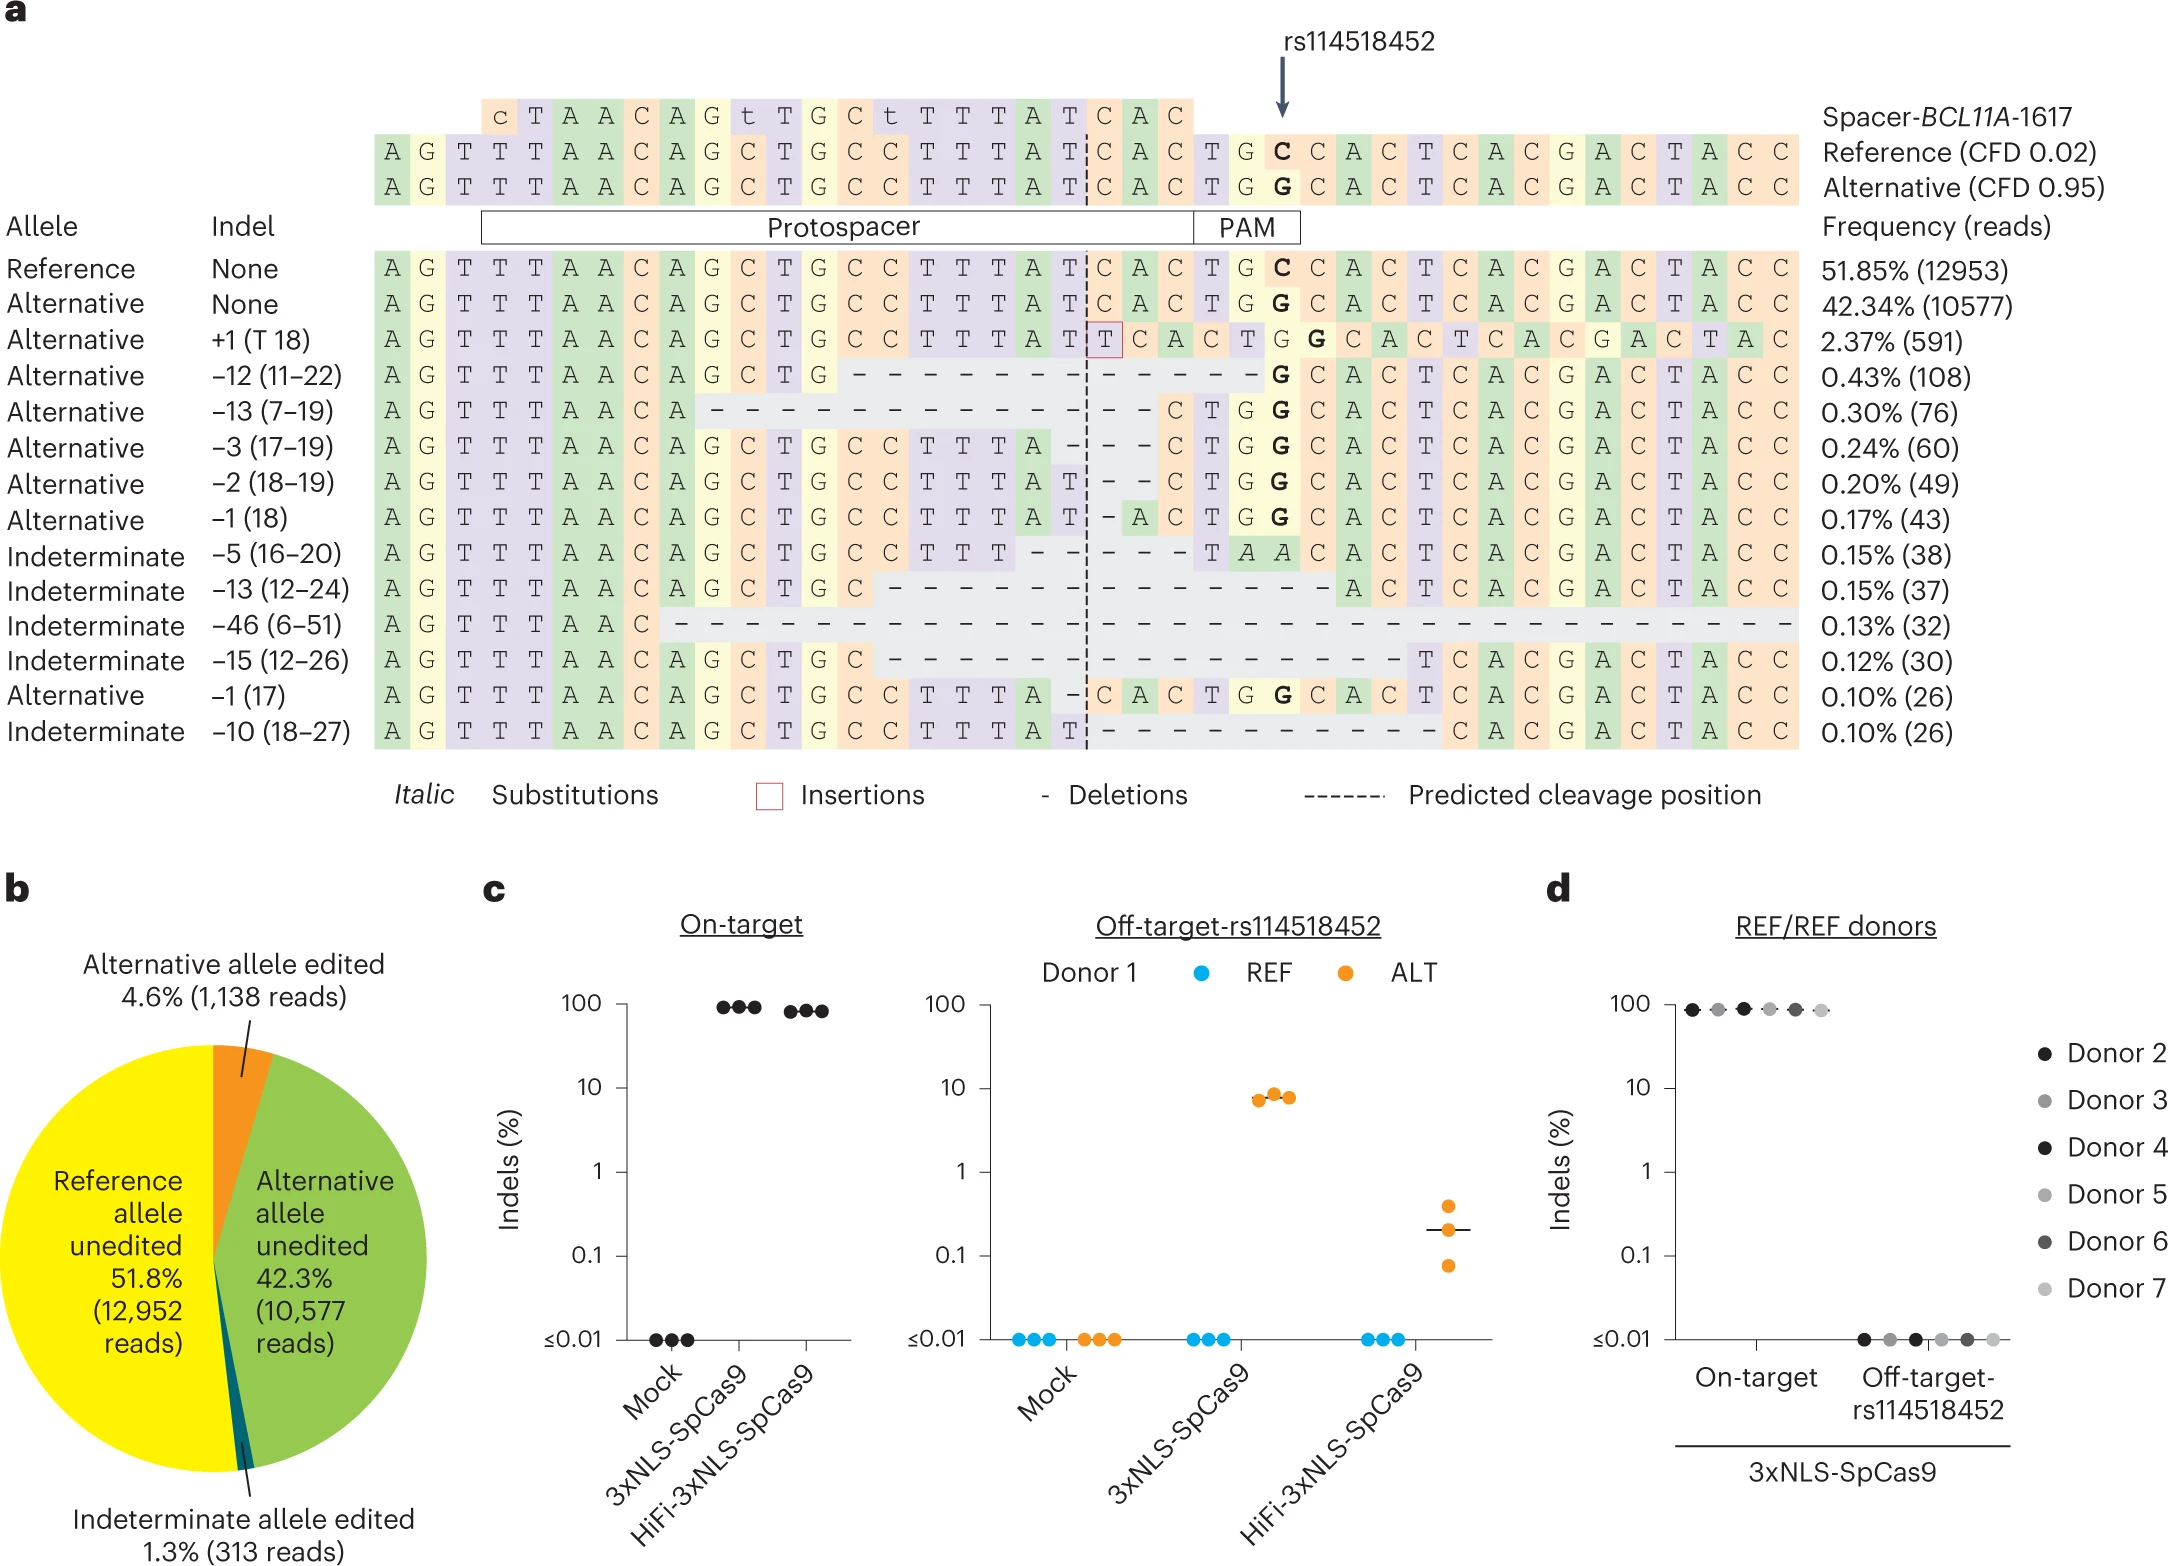
\includegraphics[width=\textwidth]{figures/crisprme6.png}
	\caption[Allele-specific off-target editing by a BCL11A enhancer targeting gRNA in clinical trials associated with a common variant in African-ancestry populations]{\textbf{Allele-specific off-target editing by a BCL11A enhancer targeting gRNA in clinical trials associated with a common variant in African-ancestry populations. (A)} Human CD34+ HSPCs from a donor heterozygous for rs114518452-\texttt{G}/\texttt{C} (Donor 1, REF/ALT) were subject to 3xNLS-SpCas9:sg1617 RNP electroporation followed by amplicon sequencing of the off-target site around chr2:210,530,659-210,530,681 (off-target-rs114518452 in 1-start hg38 coordinates). CFD scores for the reference and alternative alleles are indicated and representative aligned reads are shown. Spacer shown as DNA sequence for ease of visual alignment, with mismatches indicated by lowercase and the rs114518452 position shown in bold. \textbf{(B)} Reads classified based on allele (indeterminate if the rs114518452 position is deleted) and presence or absence of indels (edits). \textbf{(C)} Human CD34+ HSPCs from a donor heterozygous for rs114518452-\texttt{G}/\texttt{C} (Donor 1) were subject to 3xNLS-SpCas9:sg1617 RNP electroporation, HiFi-3xNLS-SpCas9:sg1617 RNP electroporation, or no electroporation (mock) followed by amplicon sequencing of the on-target and off-target-rs114518452 sites. Each dot represents an independent biological replicate ($n = 3$). Indel frequency was quantified for reads aligning to either the reference or alternative allele. \textbf{(D)} Human CD34+ HSPCs from 6 donors homozygous for rs114518452-\texttt{G}/\texttt{G} (Donors 2-7, REF/REF) were subject to 3xNLS-SpCas9:sg1617 RNP electroporation with 1 biological replicate per donor followed by amplicon sequencing of the on-target and off-target-rs114518452 sites.}
	\label{fig:crisprme6}
\end{figure} 
The on-target BCL11A intronic enhancer site is on chr2p while the off-target-rs114518452 site is on chr2q within an intron of a non-canonical transcript of CPS1. Inversion PCR demonstrated inversion junctions consistent with the presence of $\sim 150$ Mb pericentric inversions between BCL11A and the off-target site only in edited HSPCs carrying the alternative allele (Fig. 4a,b). Deep sequencing of the inversion junction showed that inversions were restricted to the alternative allele in the heterozygous cells (\textbf{Fig.\ref{fig:crisprme7} (C)} and \textbf{(D)}). Droplet digital PCR revealed these inversions to be present at $0.16 \pm 0.04\%$ allele frequency (\textbf{Fig.\ref{fig:crisprme7} (E)}). 
\begin{figure}
	\centering
	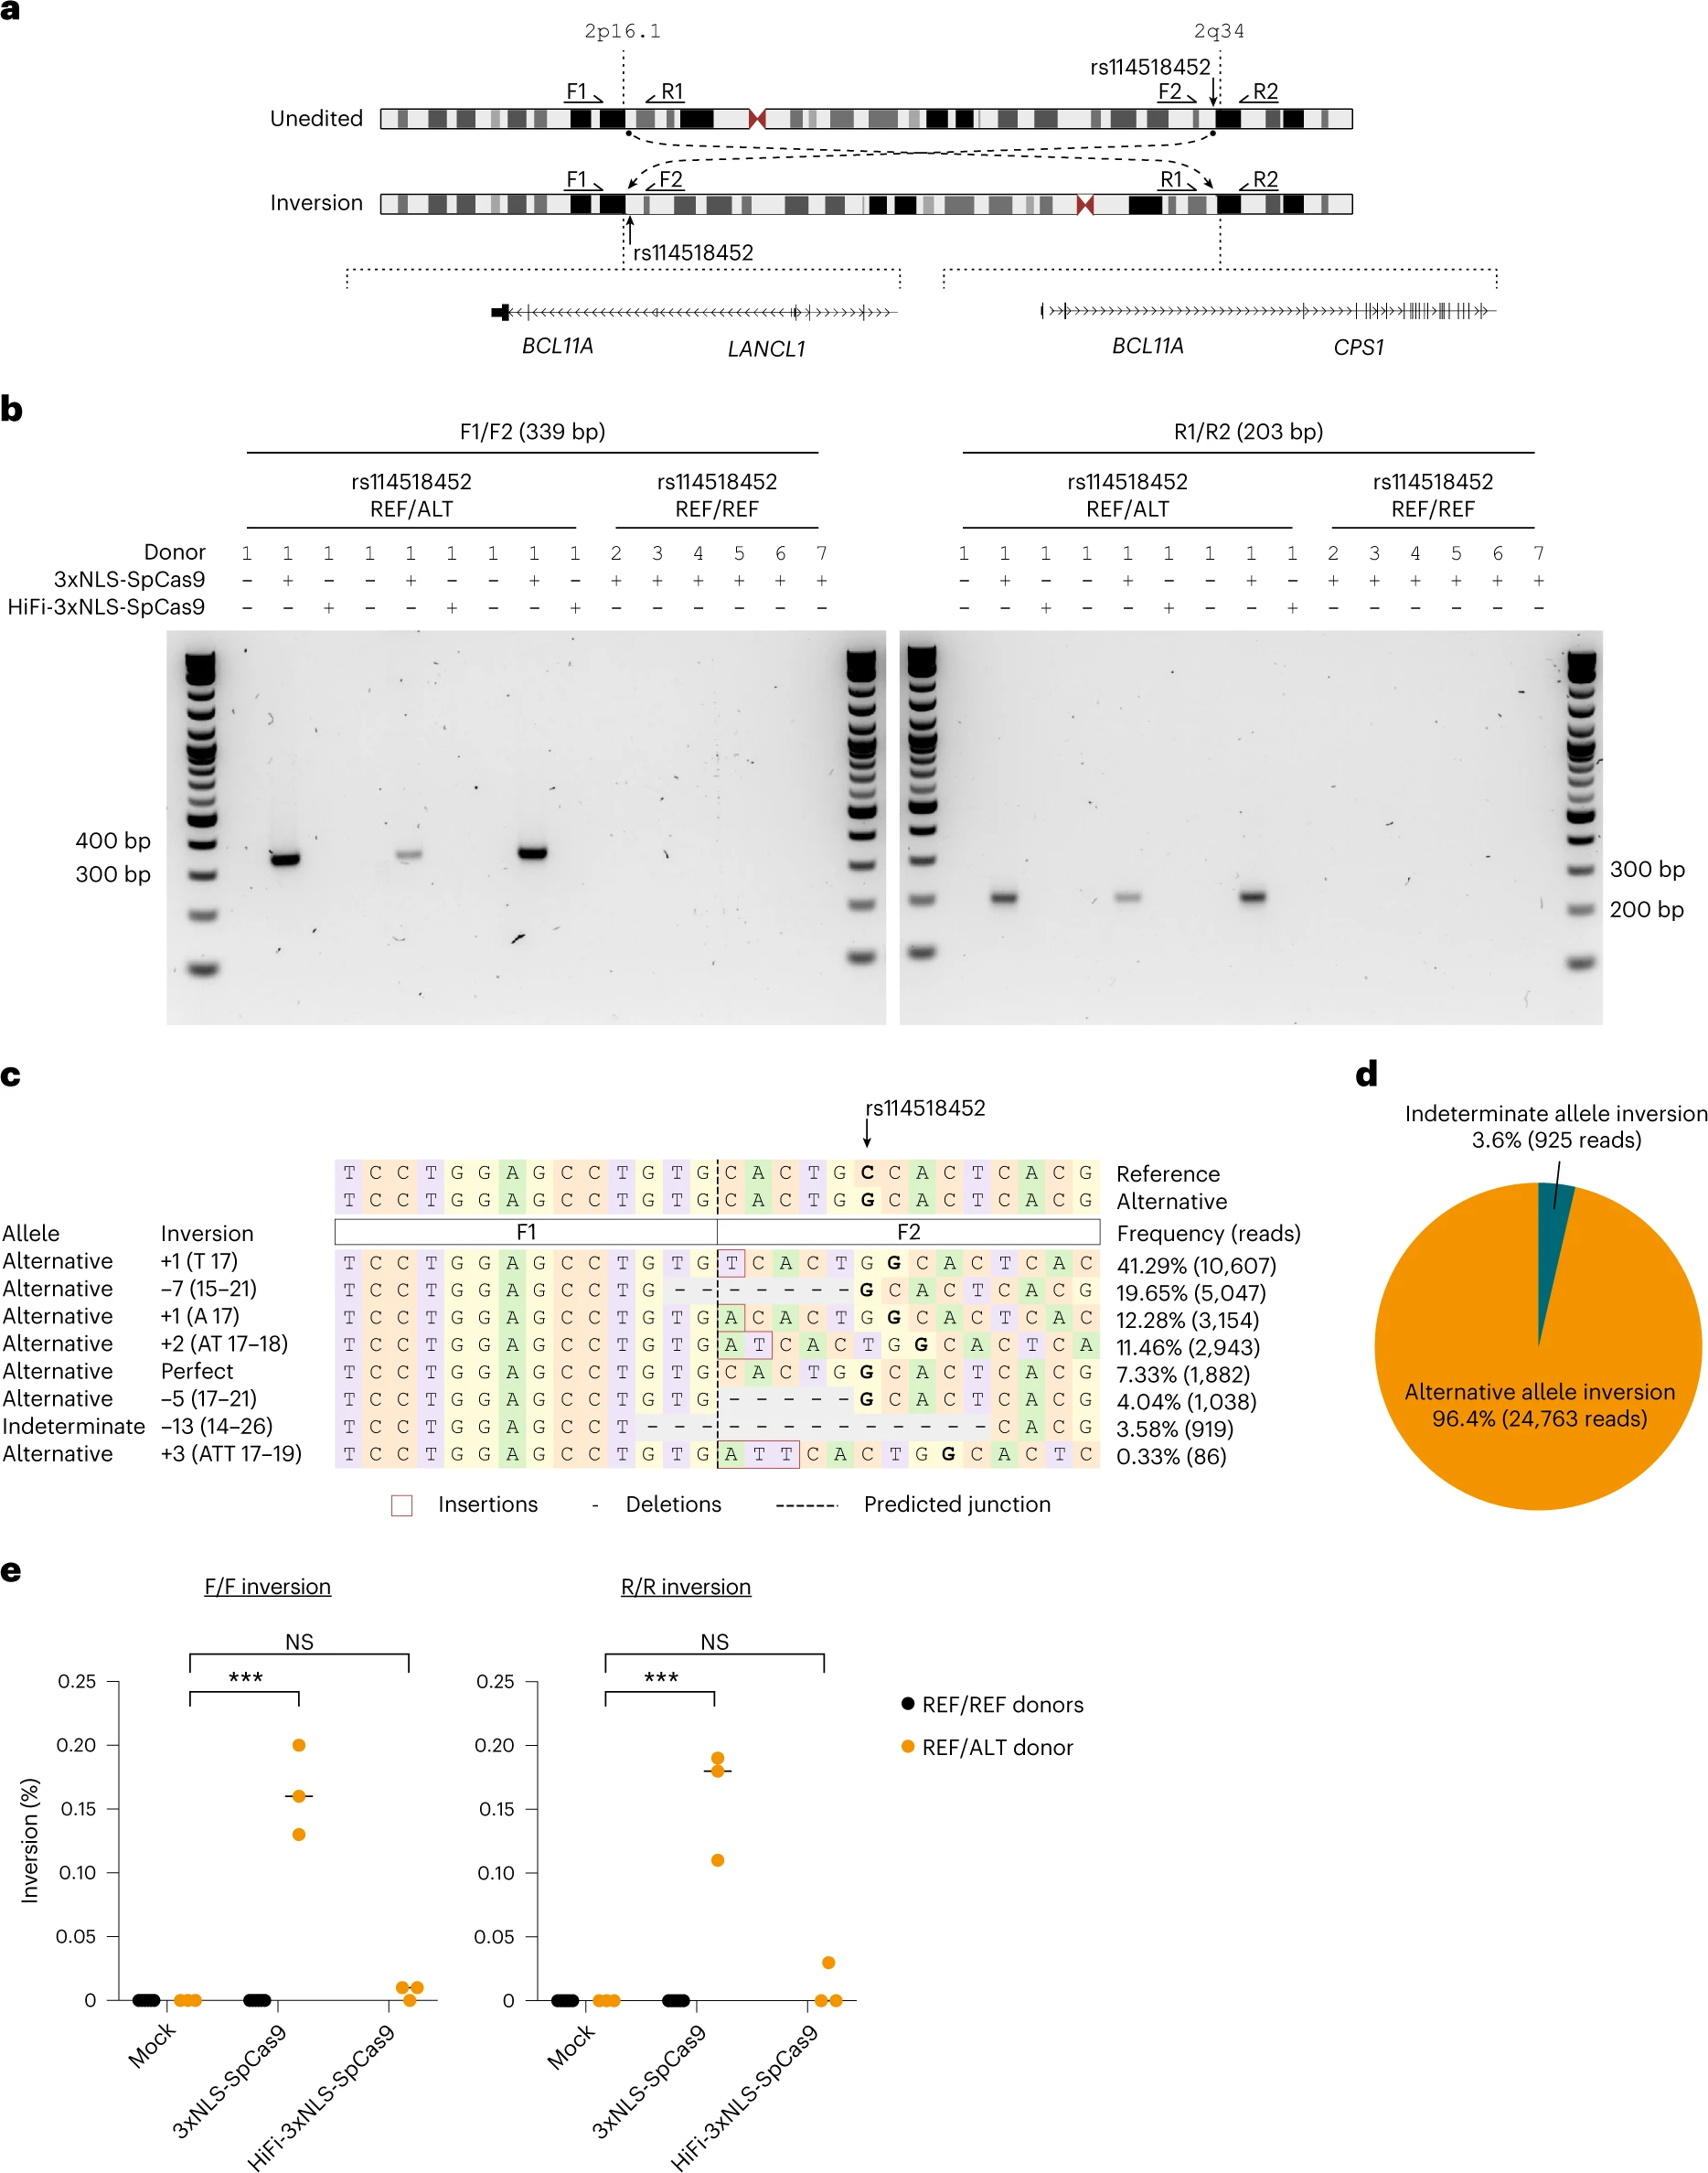
\includegraphics[width=\textwidth]{figures/crisprme7.png}
	\caption[Allele-specific pericentric inversion following BCL11A enhancer editing due to off-target cleavage]{\textbf{Allele-specific pericentric inversion following BCL11A enhancer editing due to off-target cleavage. (A)} Concurrent cleavage of the on-target and off-target-rs114518452 sites could lead to pericentric inversion of chr2 as depicted. PCR primers F1, R1, F2, and R2 were designed to detect potential inversions. \textbf{(B)} Human CD34+ HSPCs from a donor heterozygous for rs114518452-\texttt{G}/\texttt{C} (Donor 1) were subject to 3xNLS-SpCas9:sg1617 RNP electroporation, HiFi-3xNLS-SpCas9:sg1617 RNP electroporation, or no electroporation with 3 biological replicates. Human CD34+ HSPCs from 6 donors homozygous for rs114518452-\texttt{G}/\texttt{G} (Donors 2-7, REF/REF) were subject to 3xNLS-SpCas9:sg1617 RNP electroporation with 1 biological replicate per donor. Gel electrophoresis for inversion PCR was performed with F1/F2 and R1/R2 primer pairs on left and right respectively with expected sizes of precise inversion PCR products indicated. \textbf{(C)} Reads from amplicon sequencing of the F1/F2 product (expected to include the rs114518452 position) from 3xNLS-SpCas9:sg1617 RNP treatment were aligned to reference and alternative inversion templates. The rs114518452 position is shown in bold. \textbf{(D)} Reads classified based on allele (indeterminate if the rs114518452 position deleted). \textbf{(E)} Inversion frequency by ddPCR from same samples as in \textbf{(B)}. F/F indicates forward and R/R reverse inversion junctions as depicted in \textbf{(A)}.}
	\label{fig:crisprme7}
\end{figure} 
Various high-fidelity Cas9 variants may improve the specificity of gene editing, although at the possible cost of reduced efficiency \citep{schmid2020highly}. Gene editing following the same electroporation protocol using a HiFi variant 3xNLS-SpCas9 (R691A) \citep{vakulskas2018high} in heterozygous cells revealed $82.3 \pm 1.6\%$ on-target indels with only $0.1 \pm 0.1\%$ indels at the rs114518452-\texttt{C} off-target site, i.e. a $\sim 48$-fold reduction compared to SpCas9 (\textbf{Fig.\ref{fig:crisprme6} (C)}). Inversions were not detected following HiFi-3xNLS-SpCas9 editing (\textbf{Fig.\ref{fig:crisprme7} (B)} and \textbf{(E)}). 

To examine the pervasiveness of alternative allele off-target potential, we evaluated an additional 13 gRNAs in clinical development or otherwise widely used for SpCas9-based nuclease or base editing \citep{xu2017crispr,xu2019crispr,stadtmauer2020crispr,gillmore2021crispr,dewitt2016selection,xu2019editing,metais2019genome,tsai2015guide,zeng2020therapeutic,musunuru2021vivo} and 6 gRNAs for non-SpCas9-based editing such as for SaCas9 and Cas12a \citep{xu2019editing,chu2021rationally,newby2021base,maeder2019development,de2019edit}. CRISPRme analysis including the 1000G and HGDP genetic variant datasets showed $18\%$ ($95\%$ confidence interval $13-23\%$) of the total nominated off-targets were due to alternative allele-specific off-targets. Most alternative allele-specific off-targets were associated with rare variants (MAF $< 1\%$), although candidate off-targets associated with common variants were identified for each gRNA (\textbf{Fig.\ref{fig:crisprme8} (A)}). None of these alternative allele-specific off-target sites were described in the original manuscripts reporting the editing strategies and off-target analyses. 
\begin{figure}
	\centering
	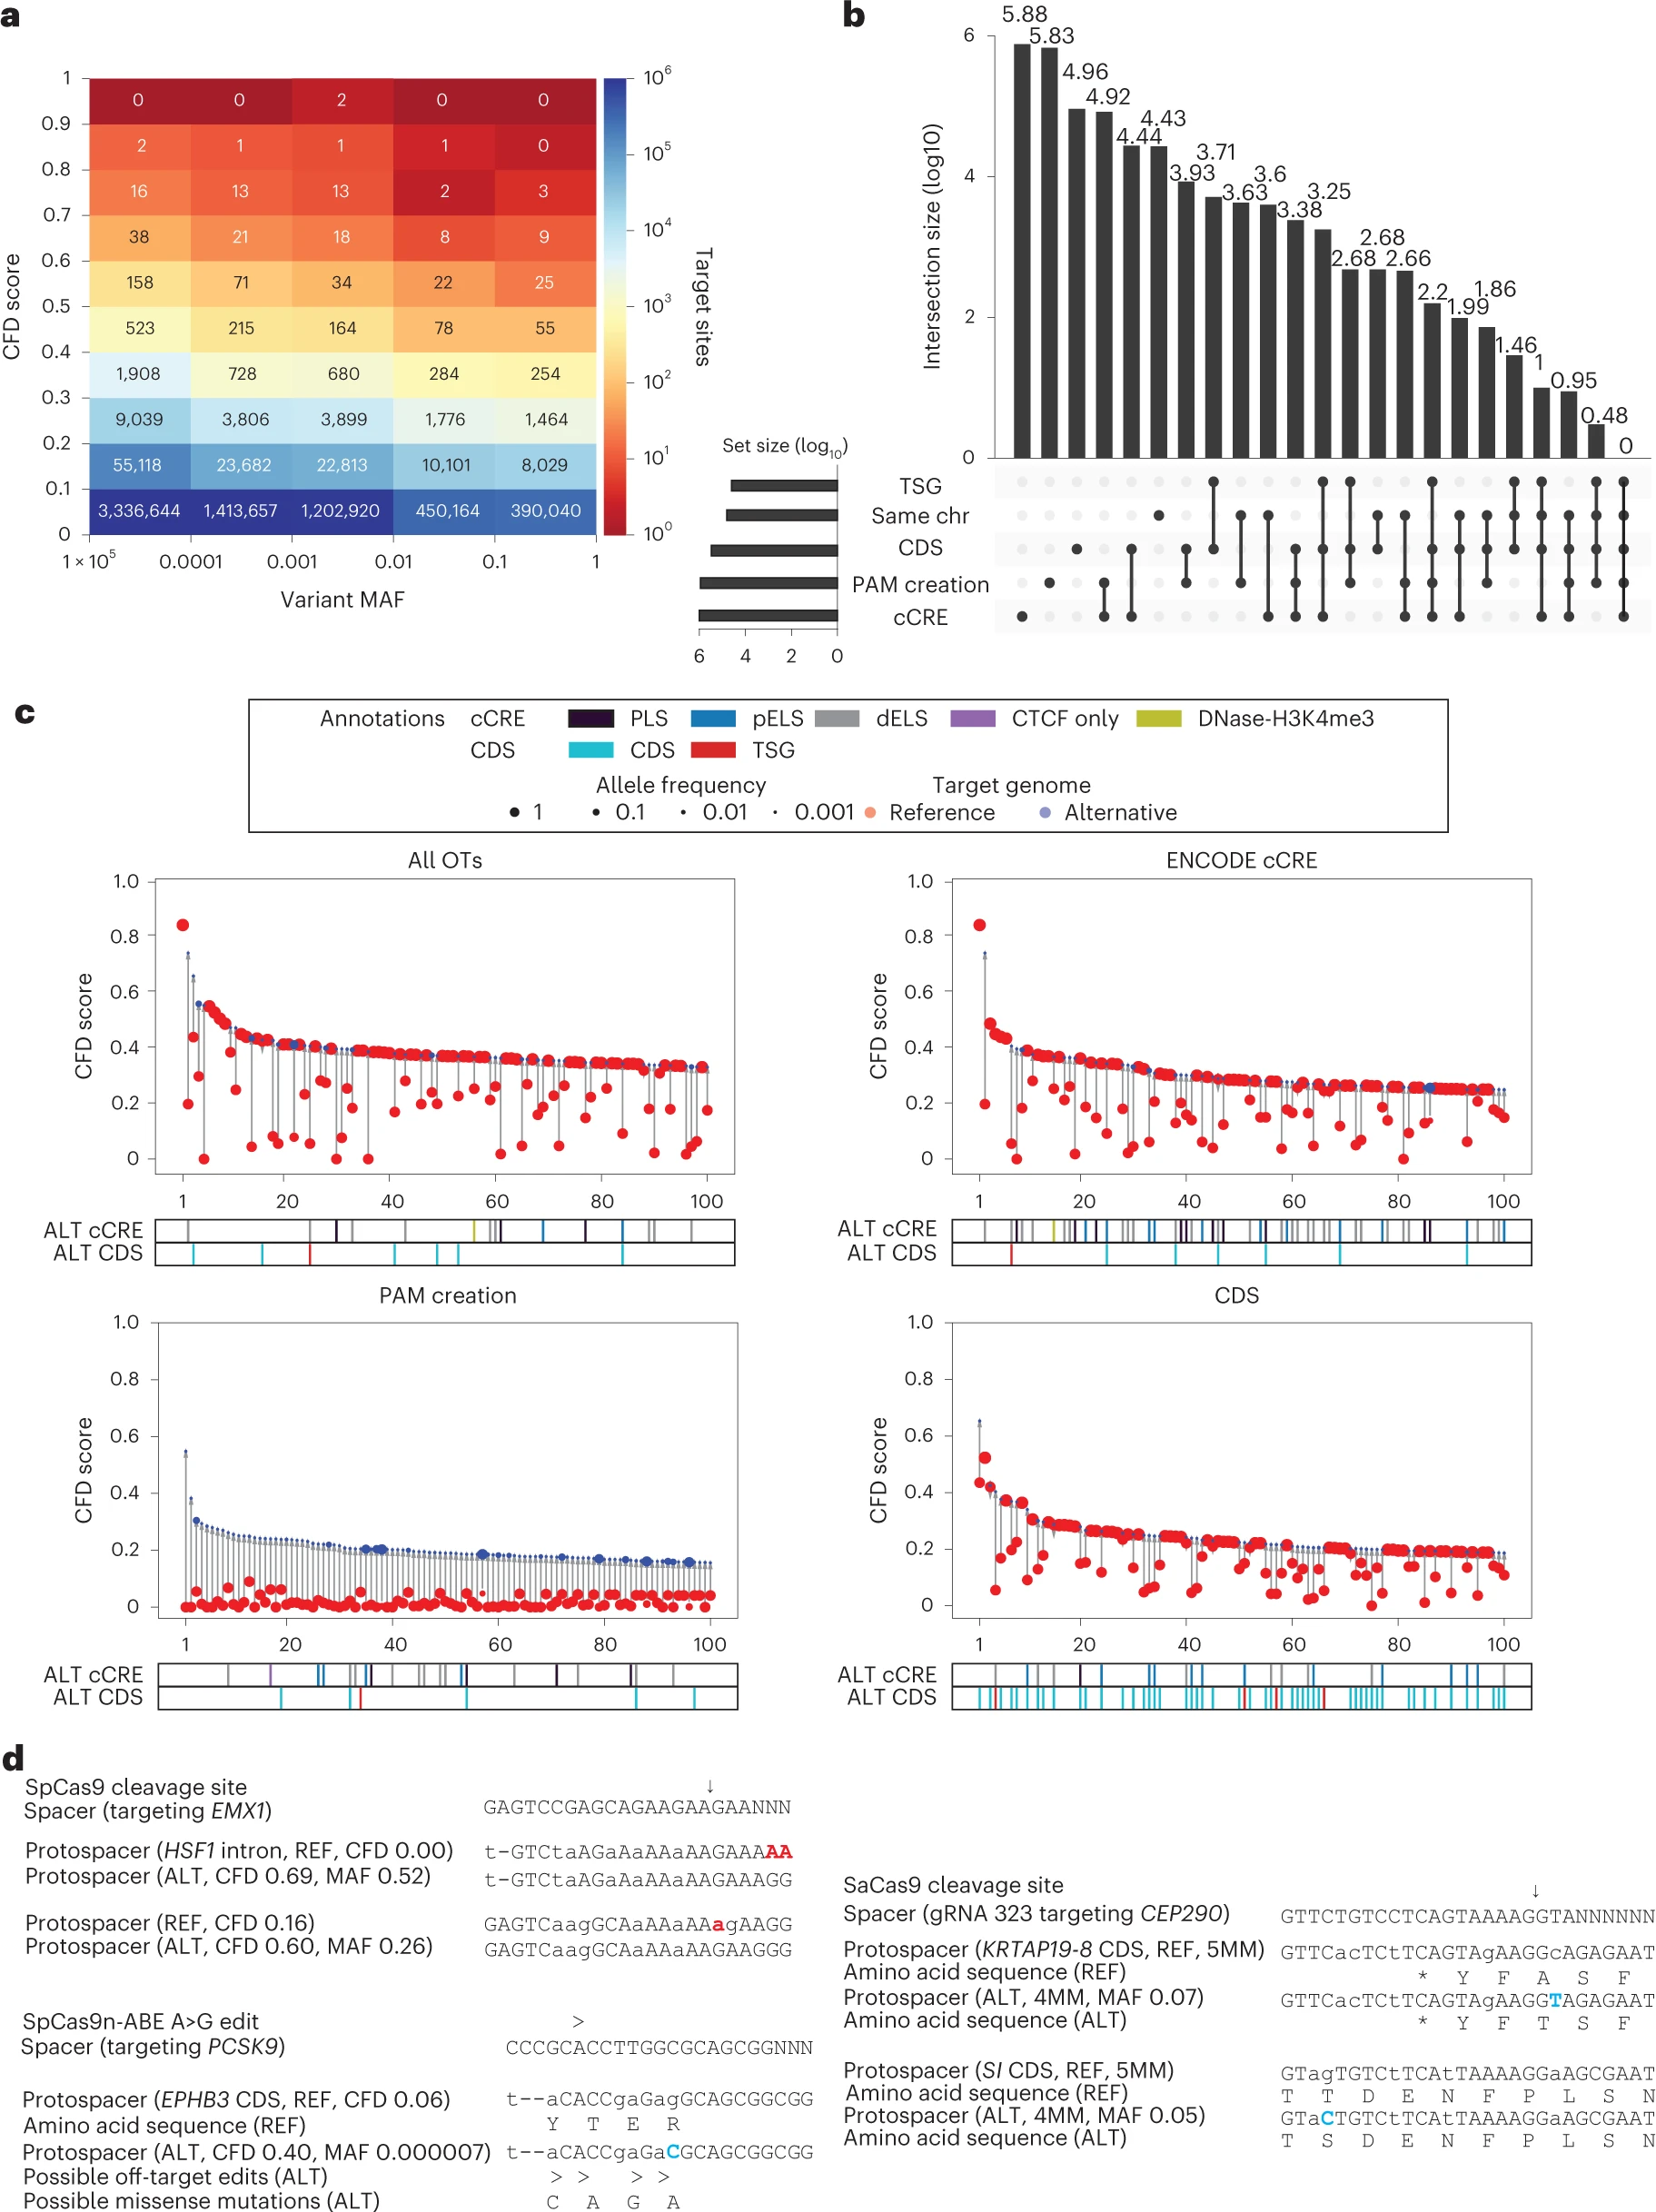
\includegraphics[width=\textwidth]{figures/crisprme8.png}
	\caption[CRISPRme illustrates prevalent off-target potential due to genetic variation]{\textbf{CRISPRme illustrates prevalent off-target potential due to genetic variation. (A)} Heatmap showing the distribution of alternative allele nominated off-targets for SpCas9 guides by CFD score and MAF. \textbf{(B)} UpSet plot showing overlapping annotation categories for candidate off-targets (TSG, tumor suppressor gene; candidate off-targets on the same chromosome as the on-target; CDS regions; cCRE from ENCODE and PAM creation events). \texttt{(C)} Top 100 predicted off-target sites ranked by CFD score for the gRNA targeting PCSK9 with no filter, found in cCREs, corresponding to PAM creation events, and in CDS regions) \texttt{(D)} Top left: Candidate off-target sites with increased predicted cleavage potential introduced by common (MAF $52\%$ and $26\%$) indel variants for a SpCas9 gRNA targeting EMX1. Right: Candidate off-target cleavage sites within coding sequences with increased homology to a lead gRNA for SaCas9 targeting of CEP290 to treat congenital blindness in current clinical trials due to common SNPs. Bottom: Potential missense mutations in the EPHB3 tumor suppressor resulting from candidate off-target \texttt{A}-to-\texttt{G} base editing by a preclinical lead gRNA targeting PCSK9 to reduce LDL cholesterol levels. Deletions shown in red, SNPs shown in blue.}
	\label{fig:crisprme8}
\end{figure} 
CRISPRme produces visualizations to specifically highlight alternative allele-specific candidate off-target sites overlapping candidate cis-regulatory elements and protein coding sequences (including putative tumor suppressor genes \citep{zhao2016tsgene}) and/or which involve PAM creation events (\textbf{Fig.\ref{fig:crisprme8} (B-C)}). For example, within the top 20 candidate off-targets nominated by CRISPRme for a SpCas9 gRNA targeting EMX135, two sites involve genetic variants with high MAF ($52\%$ and $26\%$) and are associated with substantial increases in CFD score from REF to ALT ($+0.69$ and $+0.44$). The first is an intronic PAM creation variant, while the second introduces two PAM-proximal matches to the gRNA (\textbf{Fig.\ref{fig:crisprme8} (D)}). Notably, both of these candidate off-targets involve indel variants, underscoring the utility of CRISPRme to account for variants beyond SNPs. In addition to visualizing candidate off-target sites by predictive score rank (such as CFD or CRISTA) for SpCas9 derived editors, CRISPRme can also visualize candidate off-targets by number of mismatches and bulges, which may be especially useful for Cas proteins with distinct PAMs for which predictive scores are not readily available. For example, SaCas9 is a clinically relevant nuclease whose small size favors packaging to AAV. For a SaCas9-associated gRNA targeting CEP29040 currently being evaluated in clinical trials to treat a form of congenital blindness (NCT03872479), CRISPRme nominated two candidate off-targets associated with common SNPs (MAF $7\%$ and $5\%$) that reduced mismatches from 5 (REF) to 4 (ALT) which are predicted to produce cleavages within coding sequences (\textbf{Fig.\ref{fig:crisprme8} (D)}). CRISPRme can nominate variant off-targets for base editors and evaluate their base editing susceptibility within a user-defined editing window. For a gRNA targeting PCSK937 that has been used with SpCas9-nickase adenine base editor in vivo in preclinical studies to reduce LDL cholesterol levels, 4 of the top 5 candidate off-target sites involve alternative alleles, including one with CFDref $0.2$ and CFDalt $0.75$ found in an ENCODE candidate enhancer element. CRISPRme nominated a candidate off-target associated with a rare variant (MAF $0.0007\%$) that increased the CFD score from $0.06$ (REF) to $0.40$ (ALT) which would be predicted to produce missense mutations in EPHB3, a putative tumor suppressor gene (\textbf{Fig.\ref{fig:crisprme8} (D)}). The underlying computational challenge that CRISPRme addresses extends beyond CRISPR-based applications to other technologies based on nucleic acid sequence recognition. For example, CRISPRme can nominate off-targets for RNA-targeting strategies, whether RNA-guided gene editors or even oligonucleotide sequences used as RNA interference (RNAi) or antisense oligo (ASO) therapies (\textbf{Fig.\ref{fig:crisprme9}}). 
\begin{figure}
	\centering
	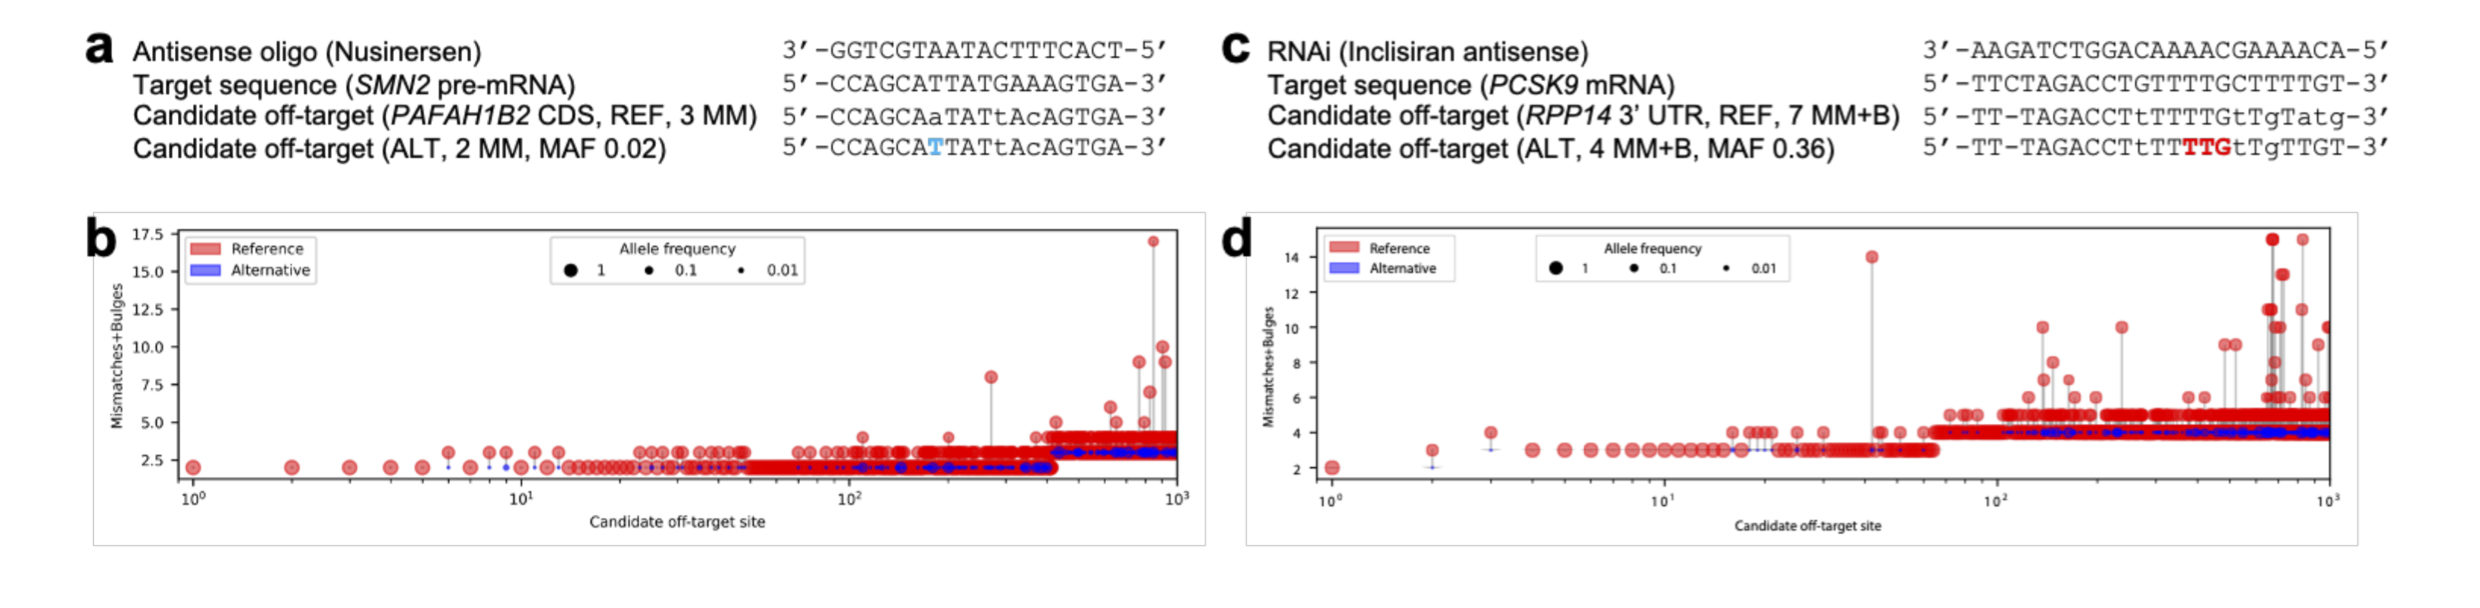
\includegraphics[width=\textwidth]{figures/crisprme9.png}
	\caption[Candidate transcript off-targets introduced by common genetic variants for non-CRISPR sequence-based RNA-targeting therapeutic strategies]{\textbf{Candidate transcript off-targets introduced by common genetic variants for non-CRISPR sequence-based RNA-targeting therapeutic strategies. (A)} A common SNP (in blue) introduces a candidate CDS off-target site with 2 mismatches for the FDA-approved antisense oligo Nusinersen. \textbf{(B)} Top 1000 candidate transcript off-targets ranked by mismatches and bulges for Nusinersen from a search performed with the 1000G and HGDP genetic variant datasets. \textbf{(C)} A common insertion variant (in red) introduces a candidate 3’UTR off-target site with 4 mismatches + bulges for the FDA-approved RNAi therapy Inclisiran. \textbf{(D)} Top 1000 candidate transcript off-targets ranked by mismatches and bulges for Inclisiran from a search performed with the 1000G and HGDP genetic variant datasets.}
	\label{fig:crisprme9}
\end{figure} 
We performed a variant-aware search (without PAM restriction) for the FDA-approved antisense oligonucleotide Nusinersen \citep{finkel2017nusinersen,mercuri2018nusinersen}, which targets SMN2 pre-mRNA to treat spinal muscular atrophy. Using CRISPRme, we identified a potential off-target site within a coding region wherein a common SNP (MAF $2\%$) reduces the number of mismatches from 3 (REF) to 2 (ALT). Similarly, analysis of the FDA-approved RNAi therapy Inclisiran \citep{raal2020inclisiran}, which targets PCSK9 mRNA to treat hypercholesterolemia, revealed that its antisense strand has a candidate off-target in the 3’ UTR of the ribosomal gene RPP14 for which a common insertion variant (MAF $36\%$) reduces the number of mismatches and bulges from 7 (REF) to 4 (ALT).
% ------ Future directions
\mychapter{8}{Future directions}
In the next future, we plan to improve the Motif Graph framework by developing a more efficient and powerful model training procedure, which will accounts for $k$-mers weights when assigning the scores on the $G$ edges. Moreover, we plan to speed-up the Motif Graph training procedure potenbtially emplyoing string indexing algorithms, like Suffix Arrays or BWT. We plan to integrate the kernel and model training procedures in a single software implementation and extensively test the newly obtained framework on different TFBS data sources , such as ChIP-seq, HT-SELEX, PBM, etc.

In the next months we plan to implement MotifRaptor2 in a comprehensive software suite, and to extensively test the framework on different GWAS datasets, cell-types, and TFs.

We plan to extend CRISPRme framework to account for complex genetic mutation events, such as indels and structural variations. To accomplish this task, we plan to extend CRISPRme search to search off-targets on genome graph data structures, which handle indels and structural variations by definition. Moreover, we also plan to extend CRISPRme to analyze the transcriptome beside the genome. Analyzing the transcriptome would enable to directly estimate potential off-targets on the genome coding regions.

% ------  begin bibliography
\bibliography{biblio}
\bibliographystyle{natbib}





\end{document}